\documentclass[a4paper]{thesis}

\def\StudiengangTitel{Masterstudiengang Philosophie}

\def\Studiengang{Philosophie M. A.}

\def\Semester{6}

\def\DeinName{Alexander Max Bauer}

\def\DeineMartrikelnummer{}

\def\ErsteAdressezeile{}

\def\ZweiteAdressezeile{}

\def\DeineEmail{alexander.max.bauer@uni-oldenburg.de}

\def\DeineTelefonnummer{}

\author{\DeinName}
\def\TitelDerArbeit{Monotonie und Sensitivität als Desiderata für Maße der Bedarfsgerechtigkeit}

\def\Untertitel{Zu zwei Aspekten der Grundlegung empirisch informierter Maße der Bedarfsgerechtigkeit zwischen normativer Theorie, formaler Modellierung und empirischer Sozialforschung}

\def\Abschlussarbeit{Masterarbeit}

\def\AkademischerGrad{\textit{Master of Arts} (M.A.)}

\def\Fachbezeichnung{Philosophie}

\def\Gutachterinnen{Gutachter}

\def\ErsteGutachterin{Prof. Dr. Mark Siebel}

\def\ZweiteGutachterin{Dr. Arne Weiß}

\def\Stichwoerter{}

\def\Thema{}

\def\Datum{\today}

\def\SeitenrandLinks{2.5cm}

\def\SeitenrandRechts{3cm}

\def\SeitenrandOben{2.5cm}

\def\SeitenrandUnten{2.5cm}
\DeclareAcronym{LaTeX}{
short = \LaTeX,
long = Lamport TeX
}

\begin{document}

\begin{titlepage}
\begin{otherlanguage}{ngerman}
\onehalfspacing
\pagenumbering{Roman}
\newgeometry{top=2.28cm,bottom=2.28cm,left=\SeitenrandLinks,right=\SeitenrandLinks}
\begin{center}
\begin{figure}[t]
\makebox[\textwidth]{\includegraphics[scale=0.15]{titlepage/figures/logo.pdf}}
\end{figure}
{\Large \textbf{Monotonie und Monotoniesensitivität als Desiderata für Maße der Bedarfsgerechtigkeit}}\\[0.5cm]
{\large \textbf{Zu zwei Aspekten der Grundlegung empirisch informierter Maße der Bedarfsgerechtigkeit zwischen normativer Theorie, formaler Modellierung und empirischer Sozialforschung}}\\[2cm]
\makebox[\textwidth]{\includegraphics[scale=0.45]{titlepage/figures/bacciarelli_themis.jpg}}\\[1cm]
{\large \textbf{\DeinName}}\\[0.5cm]
Januar 2018\\[0.5cm]
Titelabbildung:\\
Marcello Bacciarelli -- Themis
\end{center}
\end{otherlanguage}
\end{titlepage}
\restoregeometry
\MSonehalfspacing
\cleardoublepage
\setcounter{savepage}{\arabic{page}}
\pagenumbering{arabic}

\Zitate{
\cleardoublepage
\begin{singlespace}
\epigraph{Die Menschheit ist bedingt durch Bedürfnisse. Sind diese nicht befriedigt, so erweist sie sich ungeduldig; sind sie befriedigt, so erscheint sie gleichgültig. Der eigentliche Mensch bewegt sich also zwischen beiden Zuständen; und seinen Verstand, den sogenannten Menschenverstand wird er anwenden seine Bedürfnisse zu befriedigen; ist es geschehen, so hat er die Aufgabe, die Räume der Gleichgültigkeit auszufüllen.}
{{\textsc{Johann Wolfgang von Goethe}}\\
Wilhelm Meisters Wanderjahre}\blfootnote{von Goethe, Johann Wolfgang: \textit{Wilhelm Meisters Wanderjahre (1829)}. In: ders.: Sämtliche Werke nach Epochen seines Schaffens. Münchner Ausgabe. Hrsg. von Karl Richter. München, Wien 1991. Bd. 17. S. 239-714. Hier: S. 527.}
\epigraph{Daß das menschliche Daseyn eine Art Verirrung seyn müsse, geht zur Genüge aus der einfachen Bemerkung hervor, daß der Mensch ein Konkrement von Bedürfnissen ist, deren schwer zu erlangende Befriedigung ihm doch nichts gewährt, als einen schmerzlosen Zustand, in welchem er nur noch der Langenweile Preis gegeben ist, [...].}
{{\textsc{Arthur Schopenhauer}}\\
Parerga und Paralipomena}\blfootnote{Schopenhauer, Arthur: \textit{Parerga und Paralipomena}. In: ders.: Arthur Schopenhauers Werke in fünf Bänden. Hrsg. von Ludger Lütkehaus. Bd. 5. S. 261f.}
\end{singlespace}
}

\cleardoublepage
\begin{singlespace}
\epigraph{Science is a collaborative enterprise spanning the generations. When it permits us to see the far side of some new horizon, we remember those who prepared the way, seeing for them also.}
{{\textsc{Carl Edward Sagan}}\\Cosmos}\blfootnote{Sagan, Carl; Druyan, Ann und Soter, Steven: \textit{Cosmos. A personal voyage}. Dreizehnteilige Fernsehserie unter der Regie von Adrian Malone,  produziert 1978 und 1979 von Gregory Andorfer und Rob McCain. Episode 5.}
\end{singlespace}
\Danksagung{
\lettrine{D}{}\thickspace er vorliegende Text stellt eine durchgesehene und leicht überarbeitete Fassung meiner Masterarbeit dar, die ich im Januar 2017 bei Mark Siebel und Arne Weiß an der Carl von Ossietzky Universität Oldenburg eingereicht habe.

Die empirische Untersuchung bildet eine Grundlage des Arbeitspapiers \enquote{Needs as reference points -- When marginal gains to the poor do not matter}, das mit Arne Weiß und Stefan Traub veröffentlicht wurde. Eine erweiterte Fassung des zweiten Kapitels soll außerdem als \enquote{Gerechtigkeit und Bedürfnis -- Versuch einer Skizze zum Begriff des Bedürfnisses vor dem Hintergrund von Bedarfsgerechtigkeit} im Oldenburger Jahrbuch für Philosophie erscheinen, das ich mit Nils Baratella herausgebe.

Diese Arbeit wäre in der vorliegenden Form ohne eine ganze Reihe von Menschen nicht denkbar gewesen. Zunächst sei sämtlichen Teilnehmerinnen und Teilnehmern an unserer Studie sowie an den Vortests zu unserer Studie sehr herzlich gedankt. Außerdem den Mitarbeiterinnen und Mitarbeitern sowie den Hilfskräften des Experimentallabors der Fakultät für Wirtschafts- und Sozialwissenschaften der Universität Hamburg sowie den Mitarbeitern des Oldenburger Labors für experimentelle Sozialforschung.

Adele Diederich, Claudia Landwehr, Stefan Liebig, Andrea Loffi, Maximilian Lutz, Malte Unverzagt und Yannic Peper danke ich ferner für Hinweise und Zugang zu Literatur.

Für entscheidende Fingerzeige sowie Gespräche und Diskussionen gilt mein Dank außerdem Meike Benker, Frank-Michael Henn, Thomas Hilbig, Jakob Koscholke, Sabine Neuhofer, Malte Meyerhuber, Nils Springhorn und Stefan Traub sowie allen an dieser Stelle nicht genannten Mitgliedern der Forschergruppe \enquote{Bedarfsgerechtigkeit und Verteilungsprozeduren} der Deutschen Forschungsgemeinschaft. Jan Romann hat darüber hinaus geholfen, auch die kompliziertesten Herausforderungen hinter \LaTeX{} zu meistern.

Mein besonderer Dank gebührt darüber hinaus Lena Zomer für ihre Geduld sowie Michael Schippers für einen entscheidenden Hinweis, ohne den diese Arbeit ihren Anfang nicht gefunden hätte.

Die empirische Forschung entstand in Zusammenarbeit mit Arne Weiß. Er und Mark Siebel standen mir stets mit gutem Rat und guter Tat zur Seite. Ohne ihre intensive Betreuung wäre diese Arbeit kaum vorstellbar gewesen. Beiden verdanke ich, dass sie für mich weit mehr als nur eine Pflichtübung wurde.

Nicht zuletzt gilt mein Dank meinen Eltern in Liebe. -- Das Gewordensein kann nur durch seine Geschichte verstanden werden. Einen großen Teil meiner Geschichte verdanke ich ihnen.}

\Inhaltsverzeichnis

\cleardoublepage
\section{Einleitung}
\lettrine{G}{}\thickspace erechtigkeit und Ungerechtigkeit bilden einen Gegensatz, der die menschliche Denkgeschichte von Alters her begleitet. Die damit verbundene Frage, wie menschliches Miteinander richtigerweise einzurichten sei, geht zurück bis an die frühen uns bekannten Wurzeln menschlicher Gesellschaft: Wir finden sie in den älteren Kulturen Ägyptens so wie Mesopotamiens, im alten Isreael ebenso wie im alten Griechenland.\endnote{Vgl. Höffe, Otfried: \textit{Gerechtigkeit. Eine philosophische Einführung}. München 2015.} Der Diskurs, der sich in den Jahrhunderten um dieses Begriffspaar entsponnen hat, scheint zunehmende Diversifikation erfahren zu haben, ohne dass in der sich hier offenbarenden Vielfalt fester Boden gewonnen worden zu sein scheint.

Neben der Gerechtigkeit im Allgemeinen sind insbesondere auch Fragen der Verteilungsgerechtigkeit im Speziellen nach wie vor allgegenwärtig. Die Problematik, wie etwas Vorhandenes zu verteilen sei, hat Denker seit Generationen beschäftigt und dabei zu zahlreichen und sehr verschiedenen normativen Theorien geführt. Diesen ist im Regelfall gemein, dass eine Person mindestens das zu erhalten habe, was ihr zustehe. Uneinigkeit hingegen wird von der Frage evoziert, was dies nun aber eigentlich sei, das einer Person zustehen sollte. Dabei haben sich in der Debatte unter anderem Gleichheit, Billigkeit, Status, Leistung und Bedarf als mögliche Kriterien herauskristallisiert, die hier ausschlaggebend sein können.\endnote{Forsyth, Donelson: \textit{Conflict}. In: ders.: Group dynamics. Belmont 2006. S. 388-389.}

Neben diesem Problem einer fundamentalen Uneinigkeit lässt sich ferner eine gewisse Ungenauigkeit des Gerechtigkeitsbegriffs für den Fall von Verteilungsproblemen ausmachen: Durch die im Regelfall rein verbale Formulierung der verschiedenen Gerechtigkeitsideale ist nicht immer klar, wie sie eigentlich auf verschiedene konkrete Verteilungssituationen anzuwenden sind. Häufig lässt sich dann nicht sagen, welchen Einfluss zum Beispiel geringe Variationen von Verteilungen auf deren Gerechtigkeitsbeurteilung haben sollen.

Während das Problem der Uneinigkeit nicht ohne weiteres lösbar scheint, ließe sich zumindest das der Ungenauigkeit auflösen, indem man die zugrundeliegenden Ideale formal durch Maße der Verteilungsgerechtigkeit modelliert, um so präzise mathematische Hilfsmittel zu erlangen, mit denen die Beurteilung verschiedener Verteilungssituationen hinsichtlich ihrer Verteilungsgerechtigkeit geleistet werden kann, wobei sie -- eine sinnvolle Konstruktion vorausgesetzt -- auch mit sehr komplexen Verteilungen oder sehr geringen Variationen in denselben zurechtkommen könnten.

In der vorliegenden Arbeit kann es -- das sollte auf der Hand liegen -- nicht darum gehen, den normativen Diskurs zu entscheiden. Was versucht werden soll, ist vielmehr, eben jenen um einige bisher wenige beachtete Aspekte zu erweitern und neben diesen inhaltlichen Versuchen auch unter methodischen Gesichtspunkten wenig ausgetretene Pfade gangbar zu machen. Dabei behandelt sie, der Titel kündigt es schon an, normative Theorie, die mit mathematischer Formalisierung und Methoden der empirischen Sozialforschung verbunden wird, wobei sie auch Forschung aus anderen Fachbereichen aufnimmt. Verfolgt wird damit ein interdisziplinärer Ansatz, der das widerzuspiegeln hofft, was Philosophie ursprünglich gemeint haben mag: Das gemeinsame, nicht an die Grenzen von Fachdisziplinen gebundene, sondern sie unter einem gemeinsamen Ziel vereinende reflexive Denken.

Dazu sollen am Beispiel der Bedarfsgerechtigkeit zwei mögliche Klassen inhaltlicher Annahmen betrachtet werden, die jeweils zur Grundlegung bei der Konstruktion der erwähnten Maße Bedeutung erlangen können: Monotonie und Monotoniesensitivität. Zunächst gilt es hierzu den begriffliche Rahmen zu spannen: Welches Verständnis von Gerechtigkeit respektive Verteilungsgerechtigkeit wird zu Grunde gelegt? Was soll unter einem solchen Maß eigentlich verstanden werden und was ist damit gemeint, dass es empirisch informiert sein soll? Auf welcher Grundlage lassen sich solche Maße schließlich konstruieren? Hier sollen mögliche Axiome aus den beiden genannten Klassen eingeführt werden, ehe in einer empirischen Untersuchung die Akzeptanz der dahinterstehenden normativen Annahmen überprüft wird. Abschließend soll mit einem Ausblick auf weitere Forschungsmöglichkeiten in diesem jungen Feld geschlossen werden.

\cleardoublepage
\section{Empirisch informierte Maße der Bedarfsgerechtigkeit}
\lettrine{G}{}\thickspace erechtigkeit ist in aller Munde; im persönlichen Gespräch beim Mittagessen wird sie genauso herangezogen wie in Ansprachen von Staatsoberhäuptern, Revolutionären oder Terroristen.\endnote{Exemplarisch denke man hier an Robespierres Rede vor dem Konvent am 5. Februar 1794, in der er Terror als eine Offenbarung der Tugend und als eine unbeugsame Form der Gerechtigkeit beschrieben hat. (Vgl. de Robespierre, Maximilien: \textit{Über die Prinzipien der politischen Moral}. In: Fischer, Peter (Hrsg.): Reden der Französischen Revolution. München 1989. S. 341-362.)} Sie ist allgemein als eine Kategorie anerkannt, die in unserer politischen Praxis wie in unserem alltäglichen Zusammenleben omnipräsent ist.\endnote{Quante etwa beschreibt unsere \enquote{Gerechtigkeitsintuition als nicht eliminierbares, zentrales Bewertungkriterium [...].} (Quante, Michael: \textit{Einführung in die Allgemeine Ethik}. Darmstadt 2013. S. 64.) Und für Höffe lässt sich aufgrund der Annahme einer \enquote{kulturen- und epochenübergreifenden, interkulturell anerkannten Gerechtigkeit [...] die gesamte Menschheit als eine Gerechtigkeitsgemeinschaft ansprechen.} (Höffe: \textit{Gerechtigkeit}. S. 11.) Diesem Universalismus entgegenstehende Position freilich finden sich im Rahmen eines moralischen Relativismus.}

Trotz oder vielleicht gerade wegen des ständigen Rekurses auf ihren Begriff ist nicht immer klar, was unter Gerechtigkeit eigentlich verstanden werden soll, weswegen zunächst das im Folgenden angenommene Verständnis derselben dargelegt wird. Um eine begründete Auseinandersetzung mit dem Begriff leisten und erste Impulse zu seiner Interpretation erlangen zu können, scheint dabei ein Rückgang auf die Geschichte des Begriffs hilfreich.

\subsection{Zu einem Begriff der Gerechtigkeit im Allgemeinen}
Anekdotisch erzählt Michael Krüger von einer Autofahrt, die er eines Frühsommers mit den alternden Philosophen Herbert Marcuse und Leo Löwenthal unternahm, um mit ihnen -- in Erinnerung an Walter Benjamin und dessen dazu verfasste Aufsätze -- das Panorama von der Schlacht am Berge Isel in Insbruck zu betrachten:

\begin{quote}
Marcuse, groß und mit zerfurchtem Gesicht, sah aus wie ein alter Indianer. Er saß vorne, der kleine Löwenthal hinten, ich fuhr. Wir sprachen Gott weiß warum über Gerechtigkeit. Plötzlich sagte Leo von hinten \enquote{Es ist gerecht, dass deine Bücher viel gelesen werden, Herbert; aber es ist ungerecht, dass meine Bücher, die viel interessanter sind als deine, so wenig gelesen werden.} Wir mussten anhalten, um uns vor Lachen schütteln zu können.\endnote{Krüger, Michael: \textit{\enquote{Suhrkamp war meine Universität.} Erinnerungen eines Verlegers}. In: Bormuth, Matthias (Hrsg.): Offener Horizont. Jahrbuch der Karl-Jaspers-Gesellschaft. Göttingen 2016. S. 145-160. Hier: S. 160.}
\end{quote}

Löwenthal leistet hier im Besonderen einen Akt, der die Menschheit seit kaum zu überblickender Zeit begleitet: Er äußert ein Urteil über Gerechtigkeit. Freilich mit einem Augenzwinkern und also nicht ganz ernst gemeint wirft es aber doch elementare Fragen auf: Warum wird der eine Umstand als gerecht, der andere als ungerecht bezeichnet? Welche Kriterien mögen hinter einem solchen Urteil stehen? Grundlegender gefragt: Was soll der Begriff der Gerechtigkeit -- nicht nur im Speziellen, sondern ganz im Allgemeinen -- eigentlich ausdrücken?

Nun gibt es eine Reihe empirischer Quellen, die aus verschiedenen Perspektiven zur Beantwortung solcher Fragen herangezogen werden können. Einigen lässt sich entnehmen, was von wem wann als gerecht klassifiziert wurde; in ihnen spiegeln sich teils die Meinungen oder Reflexionen Einzelner wieder, teils die tradierten Normen einer Gemeinschaft. Andere widmen sich der Bedeutung des Begriffs selbst. Allen gemein bleibt dabei, dass sie zuweilen wenig gemein zu haben scheinen. Nichtsdestotrotz soll versucht werden, eine vorläufige Arbeitsdefinition des Gerechtigkeitsbegriffs aus einigen exemplarischen Quellen zu gewinnen.

Vor dem Hintergrund ausgewählter Quellen wird zunächst deutlich, dass Gerechtigkeit einen relationalen Charakter zu haben scheint. Dieser zeigt sich zum Beispiel bei Platon, wenn er in den \textit{Nomoi} von einer arithmetischen und einer geometrischen Gerechtigkeit spricht; einer Gleichverteilung von gewissen Freiheiten und Rechten sowie einer Verteilung entsprechend einem angemessenen Verhältnis.\endnote{Vgl. Platon: \textit{Die Gesetze}. In: ders.: Sämtliche Werke in drei Bänden. Hrsg. von Erich Loewenthal. Darmstadt 2004. Bd. 3. S. 215-663. Hier: S. 387-388, 757b-758a.} Sind damit noch Beziehungen zwischen Menschen bezeichnet, geht der Begriff der Gerechtigkeit in seinem relationalen Moment bei Platon darüber hinaus: Eine Ganzheit kann dann als gerecht bezeichnet werden, wenn seine Bestandteile die ihnen gemäßen Funktionen erfüllen und in einem angemessenen Verhältnis zueinander stehen,\endnote{Vgl. Platon: \textit{Der Staat}. In: ders.: Sämtliche Werke in drei Bänden. Hrsg. von Erich Loewenthal. Darmstadt 2004. Bd. 2. S. 5-407. Hier: S. 142-145, 433a-435c; 157-159, 443b-444d. Wobei sich Platon auf Simonides von Keos bezieht.} wobei eine solche Ganzheit ebenso der Kosmos wie eine Gesellschaft oder die menschliche Seele sein kann. Für den Fall des menschlichen Zusammenlebens ergibt sich als Forderung, nicht als Definition, dass entsprechend jeder das Seine bekommen beziehungsweise, ins Negative gewendet, niemandem das Seine genommen werden soll.\endnote{Vgl. ebd. S. 143, 433e.} Diese Bezogenheit auf andere findet sich auch in Aristoteles' Fassung der Gerechtigkeit als Tugend;\endnote{Vgl. Aristoteles: \textit{Nikomachische Ethik}. Hrsg. von Ursula Wolf. Reinbek 2006, 1129b.} nicht zuletzt wenn er neben dem Begriff einer allgemeinen Gerechtigkeit den der Verteilungs- sowie den der Tauschgerechtigkeit und der ausgleichenden Gerechtigkeit einführt,\endnote{Vgl. ebd. 1131b} wobei nach geometrischer oder arithmetischer Methode zu ermitteln sei, was jemandem im Positiven wie im Negativen zustehe. Ähnlich auch bei Epikur, der dieses Zustehen in einen kontraktualistischen Kontext einbettet: \enquote{Gerechtigkeit ist nicht etwas an und für sich Seiendes, sondern ein im Umgang miteinander an jeweils beliebigen Orten abgeschlossener Vertrag, einander nicht zu schädigen und sich nicht schädigen zu lassen.}\endnote{Epikur: \textit{Briefe, Sprüche, Werksfragmente}. Hrsg. von Hans-Wolfgang Krautz. Stuttgart 1980. S. 77.}

Das wird von Cicero rezipiert,\endnote{Vgl. Cicero: \textit{De legibus. Über die Gesetze}. Hrsg. von Rainer Nickel. Düsseldorf 2002. 1, 6 19. Cicero: \textit{De officiis. Vom pflichtgemäßen Handeln}. Hrsg. von Heinz Gunermann. Stuttgart 1976. I, 15.} spiegelt sich schließlich auch bei Augustinus wieder\endnote{Vgl. Augustinus: \textit{De civitate dei. The city of god}. Hrsg. von Patrick Walsh. Oxford 2005-2014. XIX, 4.} und reicht fort bis zu Rawls: \enquote{Der Gerechtigkeitsbegriff ist also für mich definiert durch seine Grundsätze für die Zuweisung von Rechten und Pflichten und die richtige Verteilung gesellschaftlicher Güter. Eine Gerechtigkeitsvorstellung ist eine Ausdeutung dieser Funktion.}\endnote{Rawls, John: \textit{Eine Theorie der Gerechtigkeit}. Frankfurt am Main 1975. S. 26.}

Damit mag, wenn auch kein materialer, so doch zumindest ein formaler Begriff der Gerechtigkeit gefunden sein: Sie meint das richtige zueinander einzelner Teile eines Ganzen, insbesondere der Menschen zueinander in einem gesellschaftlichen Rahmen. Offen bleibt dabei zunächst, worin dieses Richtige besteht und nicht zuletzt auch, wie es zu legitimieren, mithin wie der Begriff material zu bestimmen ist.

\subsection{Zu einem Begriff der Verteilungs- und Bedarfsgerechtigkeit}
Das Problemfeld der Verteilungsgerechtigkeit engt nun -- zurückgehend auf eine Unterscheidung von Aristoteles\endnote{Vgl. Aristoteles: \textit{Nikomachische Ethik}. 1131b.} -- die Frage der Gerechtigkeit auf den Fall der Verteilung eines oder mehrerer Güter zwischen Mitgliedern einer beliebig spezifizierbaren Gruppe ein. Dabei gibt es eine Vielzahl verschiedener Konzepte dazu, was einen Anspruch legitimieren und wie ein Gut entsprechend eines solchen Anspruchs verteilt werden soll.\endnote{Vgl. u. a. Boulding, Kenneth: \textit{Conflict and defense. A general theory}. New York 1962. Carens, Joseph: \textit{Equality, moral incentives and the market}. Chicago 1981. Dworkin, Ronald: \textit{What is equality? Part 1. Equality of resources}. Philosophy and Public Affairs, 10 (1981). S. 185-246. Dworkin, Ronald: \textit{What is equality? Part 2. Equality of welfare}. Philosophy and Public Affairs, 10 (1981). S. 283-345. Goodin, Robert: \textit{Utilitarianism as a public philosophy}. Cambridge 1995. Harsanyi, John: \textit{Cardinal utility in welfare economics and the theory of risktaking}. Journal of Political Economy, 61 (1953). S. 434-435. Harsanyi, John: \textit{Bayesian decision theory and utilitarian ethics}. American Economic Review, 68 (1978). S. 223-228. Miller, David: \textit{Social justice}. Oxford 1976. Miller, David: \textit{Principles of social justice}. Cambridge 1999. Sen, Amartya: \textit{Choice, welfare and measurement}. Oxford 1982. Sen, Amartya: \textit{The idea of justice}. Cambridge 2009. Walzer, Michael: \textit{Spheres of justice. A defense of pluralism and equality}. New York 1983.}

Diese Heterogenität findet sich nicht nur unter Experten, sondern trifft auch auf die Meinungen von Laien zu, wie Schwettmann feststellt: \enquote{[...] empirical studies regularly reveal heterogeneity of opinions about just distributions.}\endnote{Schwettmann, Lars: \textit{Trading off competing allocation principles. Theoretical approaches and empirical investigations}. Frankfurt am Main 2009. S. 2. Für einen Überblicke über entsprechende Experimente vgl. Cowell, Frank und Schokkaert, Erik: \textit{Risk perceptions and distributional judgments}. European Economic Review, 45 (2001). S. 941-952. Traub, Stefan; Seidl, Christian; Schmidt, Ulrich und Levati, Maria: \textit{Friedman, Harsanyi, Rawls, Boulding -- or somebody else? An experimental investigation of distributive justice}. Social Choice and Welfare, 24 (2005). S. 283-309. Gaertner, Wulf und Schokkaert, Erik: \textit{Empirical social choice. Questionnaire-experimental studies on distributive justice}. Cambridge 2012.} Verschiedentlich wird versucht, die Ergebnisse dieser breiten Debatte zu kategorisieren. Scott und Kollegen,\endnote{Vgl. Scott, John; Matland, Richard, Michelbach, Philip und Bornstein, Brian: \textit{Just deserts. An experimental study of distributive justice norms}. American Journal of Political Science, 45 (2001). S. 749-767.} Konow\endnote{Vgl. Konow, James: \textit{Which is the fairest one of all? A positive analysis of justice theories}. Journal of Economic Literature, 41 (2003). S. 1188-1239.} sowie Michelbach und Kollegen\endnote{Vgl. Michelbach, Philip; Scott, John; Matland, Richard und Bornstein, Brian: \textit{Doing Rawls justice. An experimental study of income distribution norms}. American Journal of Political Science, 47 (2003). S. 523-539.} argumentieren in diesem Zusammenhang dafür, dass eigentlich eine übersichtliche Anzahl von nur vier Verteilungsprinzipien dieser Vielzahl von Positionen zugrundeliegt: Gleichheit, Effizienz, Verantwortung und Bedarf. Theorien der Verteilungsgerechtigkeit ließen sich dann klassifizieren entsprechend ihrer Präferenz für eines dieser Prinzipien.\endnote{Bei Forsyth findet sich mit Gleichheit, Billigkeit, Status, Leistung und Bedarf eine abweichende Klassifizierung (Vgl. Forsyth: \textit{Conflict}.) Für einen guten, auch formalen Überblick über Theorien seit 1950 vgl. Roemer, John: \textit{Theories of distributive justice}. Cambridge und London 1996. -- Neben diesen Begründungsmomenten können exemplarisch verschiedene Verteilungsmodi angenommen werden. Einen Überblick über verschiedene Verteilungsmodi vor dem Hintergrund des Bedarfsprinzps liefert Hassoun. (Vgl. Hassoun, Nicole: \textit{Meeting need}. Utilitas, 21 (2009). S. 250-275.)}

Das Prinzip der Gleichheit kann dabei in sehr verschiedenen Versionen gefasst werden. In seiner naivsten Form verlangt es, dass die zur Verfügung stehende Menge eines Gutes zu gleichen Teilen auf die relevanten Personen verteilt wird. Doch der Begriff des Equalisandums ist freilich nicht darauf beschränkt, das zu verteilende Gut zu meinem. Sen stellt in diesem Zusammenhang die Frage: Gleichheit von was?\endnote{Vgl. Sen, Amartya: \textit{Equality of what?} In: McMurrin, Sterling (Hrsg.): Tanner lectures on human values. Cambridge 1980. S. 197-220.}

Dementgegen lässt sich das Prinzip der Effizient fassen als die Präferenz für die höchste Gesamtmenge eines Gutes bei gleichem Input oder bei fehlender Information über den Input als die Präferenz der größten Gesamtmenge schlechthin. Ein prominentes Beispiel, dass sich unter dieses Prinzip subsumieren ließe, wäre der Utilitarismus in seinen verschiedenen Ausprägungen.\endnote{Vgl. Schwettmann: \textit{Trading off competing allocation principles}. S. 10ff.}

Das Prinzip der Verantwortung hingegen ist maßgeblich vergangenheitsbezogen. In seinem Fokus liegt die Verantwortung des Individuums: Dieses soll nur die Konsequenzen der Variablen tragen, von denen gesagt werden kann, dass es selbst dafür verantwortlich ist. Entsprechend können auch Leistungs-Ansätze hierunter subsumiert werden, nach denen sich der legitime Anteil, der einer Person zusteht, an der von ihr erbrachter Leistung orientiert.

Schließlich gibt es die Kategorie des Bedarfes. Hier wird im Regelfall die Erfüllung von nichterfüllten Bedürfnissen gefordert, wobei weder die Verantwortung der Individuen noch die Menge zukünftiger Erlöse in Betracht gezogen werden.\endnote{So fordert Boulding etwa, dass eine Gesellschaft die grundlegenden Bedürfnisse ihrer Mitglieder erfüllen sollte, unabhängig von deren jeweiligen Verdiensten. (Vgl. Boulding, Kenneth: \textit{Social justice in social dynamics}. In: Brandt, Richard (Hrsg.): Social justice. Englewood Cliffs 1962. S. 73-92.)} Mit Bedürfnis ist dabei häufig so etwas wie ein soziales Minimum gemeint, das wiederum durch eine gewisse Einkommenshöhe ausgedrückt wird.\endnote{Vgl. Schwettmann: \textit{Trading off competing allocation principles}. S. 11.}

Während solche Prinzipien in der Regel je für sich genommen begründet erscheinen, treten Konflikte auf, sobald sie und die für sie relevanten Informationen nicht mehr isoliert behandelt werden, wie Sen mit einem anschaulichen Beispiel illustriert: Jemand wird von drei Jungen, die alle eine Flöte für sich beanspruchen, zu entscheiden gebeten, wer von ihnen diese schließlich erhalten soll. Sen beschreibt drei Varianten dieser Situation, die sich in den gegebenen Informationen unterscheiden. Im ersten Fall ist nur bekannt, dass einer der drei Jungen wesentlich musikalischer ist als die beiden anderen; dieser würde die Flöte also besser spielen als die übrigen und wahrscheinlich auch mehr Freude dadurch gewinnen. Utilitaristischen Überlegungen folgend mag die Entscheidung hier also zu Gunsten des begabten Jungen ausfallen. Im zweiten Fall ist nichts über solche Begabungen oder Befähigungen bekannt, sondern nur, dass einer der Jungen aktuell wesentlich weniger Freude als die beiden anderen hat. Rawls' Unterschiedsprinzip folgend könnte man hier die Flöte diesem Jungen zugestehen. Im dritten Fall sind weder Informationen zu der Begabungen oder Befähigungen noch zu dem Grad an Freude gegeben, über den die Jungen verfügen. Stattdessen ist nur bekannt, dass einer von ihnen die Flöte selbst aus einen Stück Holz gefertigt hat, das vorher niemandem gehörte, während die anderen beiden nichts dazu beigetragen haben. Hier könnte die Leistung des Jungen der ausschlaggebende Punkt sein, ihm die Flöte zuzusprechen.\endnote{Vgl. Sen, Amartya: \textit{Resources, values and development}. Oxford 1984. S. 290-291.}

Dabei müssen diese Prinzipien, auch wenn aus ihnen widersprüchliche Forderungen erwachsen, nicht immer als strikt getrennt angesehen werden: Während Rawls eine lexikographische Ordnung der Prinzipien annimmt,\endnote{Vgl. Rawls: \textit{Eine Theorie der Gerechtigkeit}.} geht Miller unter einem Rückgang auf empirische Studien davon aus, dass Individuen verschiedene Prinzipien gleichzeitig verwenden und Abwägungen zwischen ihnen vornehmen.\endnote{Vgl. Miller: \textit{Principles of social justice}.} Konow argumentiert entsprechend, dass die Gewichtung der jeweiligen Prinzipien schließlich Kontextabhängig ist.\endnote{Vgl. Konow, James: \textit{Fair and square. The four sides of distributive justice}. Journal of Economic Behavior and Organization, 46 (2001). 137-164. Konow: \textit{Which is the fairest one of all?}.} Ähnlich bei Walzer,  der davon ausgeht, dass die Gewichtung relativ zu der Sphäre der Gerechtigkeit ist, in der sich ein Individuum beweg; etwa der Familie oder dem Arbeitsplatz. Abhängig davon kann die Präferenz für ein Verteilungsprinzip variieren.\endnote{Vgl. Walzer: \textit{Spheres of justice}. Faravelli, Marco: \textit{How conext matters. A survey based experiment on distributive justice}. Journal of Public Economics, 91 (2007). S. 1399-1422. Roemer: \textit{Theories of distributive justice}.}

Im Rahmen dieser Arbeit soll sich dabei auf das -- nicht selten in seiner Bedeutung unterschätzte -- Prinzip des Bedarfs beschränkt werden, das schließlich -- auch ihm Rahmen von Maßen der Verteilungsgerechtigkeit -- einen von mehreren Bausteinen eines pluralistischen Ansatzes bilden kann, der mehrere Prinzipien -- etwa kontextabhängig -- miteinander verbindet.

\subsection{Zu einem Begriff des Bedarfs}
Häufig steht generell Gleichheit im Fokus von Fragen der Verteilungsgerechtigkeit; nicht selten eine gewisse Art ökonomischer Gleichheit. So Stratmann stellt mit Blick auf die Wohlfahrtstheorie, die experimentelle Spieltheorie sowie die verhaltensökonomische Vertragstheorie einen Fokus auf egalitäre Konzepte fest.\endnote{Vgl. Stratmann, Felix: \textit{Gleichheitsaversion. Einführung, theoretische Fundierung, Beleg und wirtschaftspolitische Implikationen}. Unveröffentlichte Dissertation an der Universität der Bundeswehr. München 2015. Für einen empirischen Blick auf die gesellschaftliche Wahrnehmung sozialer Ungleichheit vgl. Sachweh, Patrick: \textit{Deutungsmuster sozialer Ungleichheit. Wahrnehmung und Legitimation gesellschaftlicher Priviligierung und Benachteiligung}. Frankfurt am Main 2010. Sachweh, Patrick: \textit{The moral economy of inequality. Popular views on income differentiation, poverty and wealth}. Socio-Economic Review, 10 (2012). S. 419-445.}

Dabei gerät die Bedeutung anderer Prinzipien schnell in den Hintergrund. Das Konzept des Bedarfes etwa erweist sich als moralisch bedeutsam, obwohl es nur selten explizit herangezogen wird. Frankfurt etwa fest, dass es in der Regel eigentlich nicht Ungleichheit ist, die zu bemängeln ist, wenn man soziale Missstände in den Blick nimmt, sondern dass vielmehr die damit verbundene Armut der entscheidende Stein des Anstoßes sein sollte.\endnote{Vgl. Frankfurt, Harry: \textit{Ungleichheit. Warum wir nicht alle gleich viel haben müssen}. Berlin 2016.} Mehr noch, Gleichheit als solche muss noch nicht implizieren, frei von Schaden zu bleiben. Man denke hier etwa an die Möglichkeit der Herstellung von gleicher Unterversorgung, die aus egalitaristischer Perspektive durch eine Steigerung der Gleichheit auch die Gerechtigkeit einer Verteilung steigen lassen könnte, obwohl letztlich mehr Menschen als vorher unterversorgt sind (man spricht hier von der sogenannten \textit{leveling down objection}).\endnote{Vgl. Wiggins, David: \textit{An idea we cannot do without. What difference will it make (eg. to moral, political and environmental philosophy) to recognize and put to use a substantial conception of need?} In: Reader, Soran (Hrsg.): The philosophy of need. Cambridge 2005. S. 25-50. Hier: S. 38.} Bloße Gleichheit, ohne Rücksicht auf Bedarfe, so ließe sich argumentieren, bliebe ein inhaltsleerer Formalismus, der die Möglichkeit von Verelendung, solange sie nur gleich ist, billigend in Kauf nehmen muss.\endnote{Vgl. Holtug, Nils: \textit{Egalitarianism and the levelling down objection}. Analysis, 58 (1998). S. 166-174. Entsprechend urteilt Reader: \enquote{A principle aimed at preventing inequality misses what people really care about, which is that no-one should suffer unnecessary harm.} (Reader, Soran: \textit{Introduction}. In: ders. (Hrsg.): The philosophy of need. Cambridge 2005. S. 1-24. Hier: S. 6.) Und: \enquote{[...] talk of need is indispensable to any adequate normative moral theory.} (Ebd. S. 19.)} -- Darüber hinaus erweisen sich Bedürfnisse als zentral für menschliche Handlungsfähigkeit und menschliches Gedeihen.\endnote{Vgl. Nussbaum, Martha: \textit{Aristotelian social democracy}. In: Brock, Gillian (Hrsg.): Necessary goods. Our responsibilities to meet others' needs. Oxford 1998. Reader, Soran (Hrsg.): \textit{The philosophy of need}. Cambridge 2005.} Nicht zuletzt deswegen wird es häufig als eine Kernaufgabe der Regierung angesehen, ihren Bürgern die Erfüllung ihrer Bedürfnisse zu ermöglichen.\endnote{Vgl. Braybrooke, David: \textit{Meeting needs}. Princeton 1987. Nussbaum: \textit{Aristotelian social democracy}. Wiggins, David: \textit{Claims of need}. In: ders. (Hrsg.): Needs, values, truth. Oxford 1987.}

Neben solchen grundlegenden theoretischen Gesichtspunkten gibt es eine Reihe empirisch orientierter Literatur, die nahelegt, dass Bedürfnisse zumindest auch in unserem gegenwärtigen gesellschaftlichem Rahmen über einen gewissen Stellenwert verfügen: Forsé und Parodi beispielsweise haben gezeigt, dass Menschen in allen europäischen Ländern lexikographisch das Bedarfsprinzip dem der Gleichheit oder des Verdienstes vorziehen.\endnote{Vgl. Forsé, Michel und Parodi, Maxime: \textit{Justice distributive. La hiérarchie des principes selon les Européens}. Revue de l' OFCE, 98 (2006). S. 213-244.}

Was Bedürfnisse oder Bedarfe dabei im Eigentlichen meinen, ist aber alles andere als klar. Ein Blick in den \textit{Grimm} mag hier einen ersten guten Ausgangspunkt für den Versuch darstellen, sich der Bedeutung des Begriffs zu nähern, indem es die etymologischen Wurzeln offenlegt, deren Bedeutungen das Konzept versuchsweise umreißen können. Hier wird auf Henisch verwiesen,\endnote{Vgl. Grimm, Jacob und Grimm, Wilhelm: \textit{Deutsches Wörterbuch von Jacob und Wilhelm Grimm}. München 1991. Bd. 1. Sp. 1220.} der den Begriff in seinem Wörterbuch \textit{Teutsche Sprach und Weiszheit} von 1616 das erste Mal anführt, wo er sich unter dem Lemma \enquote{Bedarffen} findet: \enquote{Bedarffen}, auch \enquote{bedörffen} oder \enquote{bedürffen}, zusammengesetzt aus \enquote{be}\endnote{Eine Silbe mit der Bedeutung des lateinischen con oder com -- also mit, gemeinsam, zusammen. (Vgl. Henisch, Georg: \textit{Teutsche Sprach und Weiszheit. Thesaurus linguae et sapientiae germanicae}. Augsburg 1616. Bd. 1. Sp. 224.)} sowie \enquote{derffen},\endnote{Für darffen verweist Henisch auf das lateinische audere -- auf etwas Lust haben, auf etwas begierig sein, etwas mögen oder wollen. (Vgl. ebd. Sp. 681.)} bedeutet von Nöten oder notwendig sein. Für das Substantiv \enquote{Bedarf} schließlich wird auf das lateinische \enquote{necessitas} und \enquote{egestas} verwiesen, womit also Notwendigkeit, Unvermeidlichkeit, Zwang sowie Dürftigkeit, Armut, Elend oder Mangel an etwas gemeint sind. Außerdem wird es mit Notdurft in seiner damals entsprechend von der heutigen verschiedenen Bedeutung identifiziert.\endnote{Vgl. ebd. Sp. 230.}

Im 18. Jahrhundert setzt sich für den Begriff durch seine Verwendung in der Handelssprache schließlich eine Bedeutung im Sinne einer Nachfrage gegen die eines Mangels durch.\endnote{Vgl. Pfeifer, Wolfgang: \textit{Etymologisches Wörterbuch des Deutschen}. Berlin 1989. Bd. 1. S. 138.} Es mag vor diesem Hintergrund sinnvoll erscheinen, eine sprachliche Unterscheidung einzuführen: Vor dem oben Gesagten lässt sich \textit{Bedürfnis}, das ursprünglich synonym zu Bedarf war, begreifen im Sinne eines als bedrängend, also schwer ausweichlich empfundenen oder festgestellten Mangels,\endnote{Das heißt, er kann subjektiv oder objektiv respektive intersubjektiv sein und damit gefasst werden als \enquote{Zustand von Mangelempfindungen [...] oder als Zustand eines Mangels, der relativ zu bestimmten Normen zu definieren ist [...].} (Schwemmer, Oswald: \textit{Bedürfnis}. In: Mittelstraß, Jürgen (Hrsg.): Enzyklopädie Philosophie und Wissenschaftstheorie. Bd. 1. S. 261-263. Hier: S. 261.)} aus dem sich ein Interesse an seiner Beseitigung ergeben kann.\endnote{Damit könnte man Bedürfnisse als Teilmenge von Interesse fassen. (Vgl. Weale, Albert: \textit{Needs and interests}. In: Craig, Edward (Hrsg.): Routledge encyclopedia of philosophy. S. 752-755. Hier: S. 753.} Der \textit{Bedarf} kann dann mit von Hermann gefasst werden als die Menge der Dinge, die zur Befriedigung eines solchen Bedürfnisses gebraucht werden.\endnote{Vgl. von Hermann, Friedrich: \textit{Staatswirthschaftliche Untersuchungen}. München 1874. S. 5f.) Diese Unterscheidung im Sinne eines Schwellenwerts (man hat zum Beispiel ein Bedürfnis von zwei Litern Wasser zum Überleben) und einer Lücke (man verfügt bereits über einen Liter als hat man einen Bedarf an einem weitern Liter) unterscheidet sich von der Interpretation Müllers, der im \textit{Historischen Wörterbuch der Philosophie} einleitet mit der Unterscheidung, dass Bedürfnis in einem subjektiven Sinne -- womit er sich auf von Hermann bezieht -- das Gefühl eines Mangels bezeichne, in einem objektiven Sinne aber wiederum das Mittel zur Beseitigung desselben. (Vgl. Müller, Johann: \textit{Bedürfnis}. In: Ritter, Joachim (Hrsg.): Historisches Wörterbuch der Philosophie. Basel 1971. Bd. 1. Sp.765-767. Hier: Sp. 765.).}

Offensichtlich bezieht sich eine solche Empfindung eines Bedürfnisses nicht auf eine spezifische Sache, sondern ist ebenso wie die Befriedigung zu stiften vermögenden Bedarfe vielfältig. Hier liegt auch eine mögliche Abgrenzung von Bedürfnissen zu Wünschen: Was ein Bedürfnis befriedigt ist unabhängig von der mentalen Haltung eines Subjekts, anders als bei einem Wunsch oder Verlangen. Wenn jemand Durst verspürt, vermag ein Glas Wasser dieses Bedürfnis nach Flüssigkeit ebenso zu befriedigen wie ein Glas Apfelschorle oder eine intravenöse Flüssigkeitszufuhr. Anders wäre dies bei dem Wunsch oder Verlangen nach einem Glas Apfelschorle, das sich schwer durch eine Nadel und einen Tropf erfüllen ließe; ein Bedürfnis mag sich in Verlangen äußern, aber nicht jedes Verlangen ist umgekehrt Ausdruck eines Bedürfnisses. Angemerkt sei hier außerdem, dass freilich die gleichen Güter verschiedene Bedürfnisse zu befriedigen vermögen und verschiedene Güter die gleichen Bedürfnisse. Dabei können Bedürfnisse miteinander in Konflikt gerade, sowohl zwischen verschiedenen Personen als auch innerhalb eines Subjekts.\endnote{Vgl. Lowe, Jonathan: \textit{Needs, facts, goodness, and truth}. In: Reader, Soran (Hrsg.): The philosophy of need. Cambridge 2005. S. 161-173. Hier: S.171. Deswegen muss ein Bedarfsansatz bei Mangel oder Knappheit anwendbar sein, das heißt, wenn größerer Bedarf als Ressourcen vorhanden ist; er muss umgehen können mit Konflikten zwischen verschiedenen Bedarfsansprüchen, wobei auch die Herkunft von Knappheit moralisch unterschiedlich konnotiert sein kann. Daneben kann auch die Frage nach der Herkunft der zu verteilenden Güter freilich moralisches Gewicht haben. (Für den Begriff der Knappheit vgl. Schramme, Thomas: \textit{Gerechtigkeit und soziale Praxis.} Frankfurt am Main 2006. Schramme liefert darüber hinaus eine Auseinandersetzung mit dem Gerechtigkeitsbegriff, der normativen Theoriekonstruktion sowie der möglichen Rolle empirischer Forschung dabei. Ferner vgl. Schramme, Thomas: \textit{On the relationship between political philosophy and empirical sciences}. Anaylse \& Kritik, 30 (2008). S. 613-626.)

Die Konnotation scheint zunächst auf physischen Objekten als Gütern zu liegen, mittels derer Bedürfnisse befriedigt werden können. Der Bedarfsbegriff erschöpft sich darin aber keineswegs: Zur Bedürfnisbefriedigung sind ebenso immaterielle Güter oder Handlungen denkbar, was damit zusammenhängt, dass Bedürfnisse selbst nicht bloß körperliche Mangelzustände, sondern auch soziale oder kognitive umfassen können; etwa durch ein Gesellschaftsbedürfnis oder durch Wißbegierede (Vgl. Wenninger, Gerd (Hrsg.): \textit{Lexikon der Psychologie}. Heidelberg 2000. Bd. 1. S. 186ff.).}

Vor dem Hintergrund dieser Offenheit gibt es im historischen Diskurs eine Vielzahl verschiedener Klassifikationsversuche hinsichtlich des Bedürfnisbegriffs.\endnote{Meran zeigt diese als \enquote{Bedeutungvielfalt des Bedürfnisbegriffs} kompakt auf: \enquote{Es gibt wohl kein Verlangen, daß nicht schon einmal Bedürfnis [...] genannt worden ist. Da liegen nebeneinander: physische und psychische, materielle und geistige, primäre und sekundäre, niedere und höhere, objektive und subjektive, natürliche und künstliche, existentielle und kulturelle, individuelle und kollektive, allgemeine und besondere, wirkliche (wahre) und eingebildete (falsche), bewußte und unbewußte, permanente und wandelbare Bedürfnisse [...].} (Meran, Josef: \textit{Über einige methodische Schwierigkeiten, den Begriff \enquote{Bedürfnis} als Grundbegriff der Kulturwissenschaften zu verwenden}. In: Schöpf, Alfred (Hrsg.): Bedürfnis, Wunsch, Begehren. Probleme einer philosophischen Sozialanthropologie. Würzburg 1987. S. 17-35. Hier: S. 18.) Er versucht, diese Vielfalt in den Kulturwissenschaften zu systematisieren, indem er die Fragen nach dem Ort, an dem Bedürfnisse auftreten, sowie nach dem Abstraktionsgrad des Bedürfnisbegriffs und der Rangordnung von Bedürfnissen in den Fokus rückt. Ferner unterscheidet er zwischen vier möglichen Zwecken, denen der Begriff dient: Bedürfnisse erlangen Relevanz als erste Ursache, als letztes Datum, als oberste Norm sowie als Residualkategorie. (Vgl. ebd. S. 17ff.)

Maslow hat dann vor einem motivationstheoretischen Hintergrund ebenfalls eine Hierarchie von Bedürfnissen vorgeschlagen, die in diesem Zusammenhang sicher zu den wirkmächtigsten Modellen dieser Zeit gehört. (Vgl. Maslow, Abraham: \textit{A theory of human motivation}. Psychological Review, 50 (1943). S. 370-396.) Einen Aktualisierungsversuch der Konzeption versucht unter anderem Alderfer (Vgl. Alderfer, Clayton: \textit{An empirical test of a new theory of human needs}. Organizational Behavior and Human Performance, 4 (1969). S. 142-175.).} Dabei wurde er historisch entlang einer Reihe von Dualismen verhandelt, die hier nur auszugsweise und knapp beleuchtet werden sollen.

Einer dieser Dualismen betrifft die Frage, ob Bedürfnisse historisch oder ahistorisch, mithin ob sie statisch oder dynamisch sind: Es ließe sich vermuten, Bedürfnisse seien statisch, nur die Mittel zu deren Befriedigung -- die Bedarfe -- würden sich, zum Beispiel durch technischen Fortschritt, ändern. Oft wird allerdings davon ausgegangen, dass Bedürfnisse viel mehr auch geschichtlich dynamisch sind. Müller zum Beispiel spricht von einer Bedürfnissteigerung, -ausweitung und -entgrenzung durch merkantilistische Wirtschaftsförderung und industrielle Revolution, die historisch ganz unterschiedliche Bewertungen erfahren hat, die von einem emanzipativen und mit Kulturentwicklung verbundenen Moment, etwa bei Garve, Fichte oder Hegel, bis zur Ablehnung unter der Annahme einer kulturzerstörenden oder zumindest nachteiligen Kraft, etwa durch Novalis oder Leo, reicht.\endnote{Vgl. Müller: \textit{Bedürfnis}. Sp. 765f.} Gewisse Bedürfnisse lassen sich also als Produkt gesellschaftlicher Zusammenhänge ansehen.\endnote{Vgl. Baratta, Giorgio und Catone, Bari: \textit{Bedürfnis. II. Zur Entstehung und Entwicklung eines gesellschaftstheoretischen Bedürfnisbegriffs}. In: Sandkühler, Jörg (Hrsg.): Europäische Enzyklopädie zu Philosophie und Wissenschaften. Hamburg. 1990. S. 343-355.} Man denke hier auch an Adam Smiths Bemerkung zum Leinenhemd:

\begin{quote}
Unter lebenswichtigen Gütern verstehe ich nicht nur solche, die unerlässlich zum Erhalt des Lebens sind, sondern auch Dinge, ohne die achtbaren Leuten, selbst der untersten Schicht, ein Auskommen nach den Gewohnheiten des Landes nicht zugemutet werden sollte. Ein Leinenhemd ist beispielsweise, genau genommen, nicht unbedingt zum Leben notwendig. Griechen und Römer lebten, wie ich glaube, sehr bequem und behaglich, obwohl sie Leinen noch nicht kannten. Doch heutzutage würde sich weithin in Europa jeder achtbare Tagelöhner schämen, wenn er in der Öffentlichkeit ohne Leinenhemd erscheinen müsste.\endnote{Smith, Adam: \textit{Der Wohlstand der Nationen. Eine Untersuchung seiner Natur und seiner Ursachen}. Hrsg. von Horst Recktenwald. München 1996. S. 747.}
\end{quote}

Ein weiterer Dualismus betrifft die Frage, ob Bedürfnisse heterogen oder homogen, ob sie universell sind oder nicht.\endnote{Die historische Schule der Nationalökonomie etwa geht von einer Kulturrelativität aus. (Vgl. Müller: \textit{Bedürfnis}. Sp. 766.} Würde im Folgenden von homogenen Bedarfen ausgegangen, wäre diese Arbeit gewissermaßen redundant, das Meiste ließe sich aus der Ungleichheitsforschung unverändert auf die Überlegungen zu Bedarfen übertragen. Allein, es scheint sinnvoll, vor dem Hintergrund der Anerkennung individueller Unterschiede auch hier einen begründbaren Spielraum der Ungleichheit zuzulassen. Die folgenden Überlegungen könnten vor dem Hintergrund von Sens Frage nach dem Equalisandum freilich verstanden werden als ein Bedarfserfüllungsegalitarismus. Gemeint wäre damit, dass die heterogenen -- das ist individuell unterschiedlichen -- Bedarfe gleichermaßen erfüllt sein sollen, was durchaus eine unterschiedliche Verteilung an Mitteln bedeuten kann.

Daneben wird die Frage verhandelt, ob Bedürfnisse bloß instrumentell, damit gewissermaßen beliebig, aufzufassen sind oder ob sie einen essentiellen Teil haben, indem sie beispielsweise als abhängend von intersubjektiver Anerkennung oder objektiver Feststellbarkeit betrachtet werden.\endnote{Weale argumentiert etwa, dass Bedürfnisse objektiv beurteilbar seien: Es wäre möglich, dass jemand nicht zu einem Zahnarzt gehen möchte, aber durchaus das Bedürfnis habe, also des Besuchs bedürfe, um dadurch Heilung zu erlangen. (Vgl. Weale: \textit{Needs and interests}. S. 752f.)} Miller versucht diesbezüglich beispielsweise, bloß instrumentelle von grundlegenden Bedürfnissen zu scheiden, indem er ein besonderes Gewicht auf diejenigen Bedarfsansprüchen legt, die fundamental oder intrinsisch motiviert seien und die er an eine Lebenswichtigkeit knüpft. Er versucht dabei zu zeigen, dass unser moralisches Vokabular eine Auffassung von Bedürfnissen beinhalte, die nicht durch eine instrumentelle Interpretation fassbar sei, und die darin bestünde, etwas \textit{wirklich} zu brauchen.\endnote{Vgl. Miller, David: \textit{\enquote{To each according to his needs}}. In: ders.: Principles of social justice. Harvard 1999. S. 203-229. Hier: S. 206f.} Der Haken hierbei liegt freilich in der Interpretation dessen, was es heißen soll, etwas \textit{wirklich} zu brauchen: Ob jemand etwas wirklich braucht hängt von dem Stellenwert ab, der dem Ziel gegeben wird, vor dessen Hintergrund es gebraucht wird. Und hier stellt sich die Frage, ob es letzte Ziele gibt, deren Bedeutung indiskutabel ist, oder ob der Stellenwert solcher Ziele immer historisch, kontingeht, mithin individuell bleibt. Mit Rowe ließe sich hier sagen: \enquote{There are only things that we might generally be said to need if the circumstances dictate it, if it's good for me [...].}\endnote{Rowe, Christopher: \textit{Needs and ethics in ancient philosophy}. In: Reader, Soran (Hrsg.): The philosophy of need. Cambridge 2005. S. 99-112. Hier: S. 108f.} In diesen Zusammenhang mag auch das von Harsanyi formulierte Prinzip einer Präferenzautonomie fallen: \enquote{The principle that, in deciding what is good and what is bad for a given individual, the ultimate criteria can only be his own wants and his own preferences.}\endnote{Harsanyi, John: \textit{Morality and the theory of rational behavior}. In: Sen, Amartya und Bernard, Williams (Hrsg.): Utilitarianism and beyond. Cambridge 1982. S. 39-62. Hier: S. 55. Ferner vgl. O'Neill, John: \textit{Need, humiliation and independence}. In: Reader, Soran (Hrsg.): The philosophy of need. Cambridge 2005. S. 73-97.}

Wenn kein objektiver letzter Zweck angenommen werden kann, ließe sich dem Bedürfniss aber ein anderer essentieller Teil zusprechen, der ihn gegen Beliebigkeit absichert: Es lässt sich argumentieren, dass der empfundene Mangel -- der sich sowohl vor dem physiologischen als auch vor dem gesellschaftlichen Hintergrund entfalten kann und der in Leidempfinden resultiert -- grundlegend sein soll für den Bedarfsbegriff.\endnote{Der Begriff des Leids ist auch für den Versuch einer Definition grundlegender Bedürfnisse von Bedeutung. (Vgl. Thomson, Garret: \textit{Needs}. London 1987. Wiggins: \textit{Claims of need}.) Er kann aber auch über diesen engen Begriff hinaus Bedeutung erlangen, wie nachfolgend gezeigt werden soll. (Vgl. Gustavsson, Erik: \textit{From needs to health care needs}. Health Care Analysis, 22 (2014). S. 22-35. Hier: S. 30.)}

Dabei lässt der Begriff des Mangels und des Leids einen nicht zu unterschätzenden Interpretationsspielraum. Wie ist solches Leid zu fassen?\endnote{Vgl. Wiggins: \textit{Claims of need}.} Miller führt hier mögliche Herangehensweisen an: Schaden oder Leid lässt sich aus biologischer oder physiologischer Perspektive ebenso ableiten wie aus geteilten sozialen Normen darüber, was ein minimal annehmbares Leben konstituiert.\endnote{Vgl. Miller: \textit{\enquote{To each according to his needs}}. S. 207f. Vor dem Hintergrund gesellschaftlicher oder sozialer Normen lässt sich auch an Thomsons essentielle Natur des Menschen, (Vgl. Thomson, Garrett: \textit{Fundamental needs.} In: Reader, Soran (Hrsg.): The philosophy of need. Cambridge 2005. S. 175-186. Hier: S. 177.) Millers Fokus auf menschliche Handlungsfähigkeit (Vgl. Miller, Sarah: \textit{Need, care and obligation}. In: Reader, Soran (Hrsg.): The philosophy of need. Cambridge 2005. S. 137-160. Hier: S. 142.) oder Sens Befähigungs- oder Verwirklichungschancenansatz denken. (Vgl. Sen, Amartya: \textit{Commodities and capabilities}. Amsterdam 1985. Sen, Amartya: \textit{Capability and well-being}. In: Sen, Amartya und Nussbaum, Martha (Hrsg.): The quality of life. Oxford 1993. S. 30-53. Nussbaum, Martha: \textit{Human capabilities, female human beings}. In Nussbaum, Martha und Glover, Jonathan (Hrsg.): Women, culture, and development. A study of human capabilities. Oxford 1995. S. 61-104.)}

Die erste Möglichkeit hat den Vorzug einer möglicherweise ausschließlich empirischen Aussage, die für Urteile über Bedürfnisse eine gewisse Objektivität verspricht; man denke exemplarisch an die Möglichkeit der Nachweisbarkeit physiologischer Bedarfe oder körperlicher Mangelzustände.\endnote{Vgl. Wenninger (Hrsg.): \textit{Lexikon der Psychologie}. S. 186ff. oder an die Beschreibung des Bedürfnisses bei Lewin als Vektor im Sinne einer psychischen Kraft, der eine Größe und Richtung zukommt, und deren Stärke \enquote{grob geschätzt werden [kann] durch Anzahl und Verschiedenheit, Intensität und Dauer der Auswirkungen auf das Verhalten, das beobachtet wird.} (Murray, Henry: \textit{Bedürfnis}. In: Arnold, Wilhelm; Eysenck, Jürgen und Meili, Richard (Hrsg.): Lexikon der Psychologie. Freiburg, Basel und Wien 1971. Bd. 1. Sp. 237-239. Hier: Sp. 239. Vgl. Lewin, Kurt: \textit{Vorsatz, Wille und Bedürfnis. Mit Vorbemerkungen über die psychischen Kräfte und Energien und die Struktur der Seele}. Berlin und Heidelberg 1926. Lewin, Kurt: \textit{A dynamic theory of personality. Selected papers}. New York und London 1935.)} Allerdings muss man sich auch davor hüten, diesen Ansatz über seine Möglichkeiten hinaus zu strapazieren, und über ihn als Instanzen von Gesundheit aufzuzeigen, was letztlich vielleicht nur kontingente Ideale menschlichen Lebens sind. Denn die Konzepte von Gesundheit und Krankheit sind ihrerseits nicht so einfach fass- oder objektivierbar, wie man denken mag.\endnote{Neben dem der physiologischen sei hier außerdem auf das Konzept der psychischen Krankheit und ihrer schweren Fassbarkeit verwiesen. Vgl. Heinz, Andreas: \textit{Der Begriff der psychischen Krankheit}. Berlin 2014. Gerok, Wolfgang; Huber, Christoph; Meinertz, Thomas und Zeidler, Henning: \textit{Die innere Medizin. Referenzwerk für den Facharzt}. Stuttgart 2006. S. 4ff.) Eine solche Verknüpfung von Leid zu Gesundheit problematisiert auch Miller. (Vgl. Miller: \textit{\enquote{To each according to his needs}}. S. 208.)}

Miller schlägt vor, diesen Ansatz um die geteilten sozialen Normen zu ergänzen, die dann im Gegensatz zu individuellen Präferenzen Bedarfsansprüche begründen könnten; nicht zuletzt auch, da das Bedarfsprinzip als ein soziales Prinzip wirksam werden soll, also als eines, dass in einer Gesellschaft dazu dienen kann, leitend für deren Institutionen zu sein.\endnote{Vgl. ebd. S. 205, 211.} In diesem Sinne kann ein Bedürfnis verstanden werden als intersubjektiv anerkannte Notwendigkeit an einem Gut, um hinsichtlich einer relevanten Dimension ein minimal würdevolles Leben führen zu können. Ähnliches findet sich auch bei Kelsen:

\begin{quote}
Das Glück, das eine Gesellschaftsordnung zu garantieren vermag, kann nicht Glück in einem subjektiv-individuellen, sondern nur Glück in einem objektiv-kollektiven Sinne sein. Das heißt, unter Glück darf man nur die Befriedigung gewisser Bedürfnisse verstehen, die von der gesellschaftlichen Autorität, dem Gesetzgeber, als solche anerkannt sind, die der Befriedigung würdig sind, so wie etwa das Bedürfnis nach Nahrung, Kleidung, Behausung [...].\endnote{Kelsen, Hans: \textit{Was ist Gerechtigkeit?} Stuttgart 2016. S. 13.)}
\end{quote}

Damit lässt sich das Bedürfnis schließlich fassen als einen als bedrängend, also schwer ausweichlich empfundenen oder festgestellten Mangel, aus dem sich ein Interesse an seiner Beseitigung ergeben kann. Dieser kann als geschichtlich dynamisch und zwischen verschiedenen Individuen heterogen angenommen werden. Seine Anerkennung mag vorrangig auf eine gesellschaftlich geteilte Norm zurückgehen, wodurch sie gegen Beliebigkeit abgesichert ist. Gegenüber dem Bedürfnis fasst der Bedarf die Dinge zusammen, die zur Befriedigung eines solchen Bedürfnisses gebraucht werden können.

\subsection{Zu einem Begriff des Maßes und seiner empirischen Informiertheit}
Versucht man nun, mögliche Verteilungsmodi vor dem Hintergrund des Bedarfsprinzips als ein Maß zu formulieren, das als präzises mathematisches Hilfsmittel zur genauen Beurteilung verschiedener Verteilungssituationen hinsichtlich ihrer Verteilungsgerechtigkeit dienen soll, betritt man ein weitestgehend unbestelltes Feld der Gerechtigkeitstheorie. Abgesehen von einem rudimentären Versuch bei Miller\endnote{Vgl. Miller: \textit{\enquote{To each according to his needs}}.} sind mir noch keine Maße der Bedarfsgerechtigkeit bekannt. Bei Jasso\endnote{Vgl. Jasso, Guillermina: \textit{How much injustice is there in the world? Two new justice indexes}. American Sociological Review, 64 (1999). S. 133-168. Jasso, Guillermina: \textit{Studying justice. Measurement, estimation, and analysis of the actual reward and the just reward}. In: Törnblom, Kjell und Vermunt, Riël (Hrsg.): Distributive and procedural justice. Research and social applications. Burlington 2007. S. 225-254. Jasso, Guillermina und Wegener, Bernd: \textit{Methods for empirical justice analysis. Part 1. Framework, models, and quantities}. Social Justice Research, 10 (1997). S. 393-430.} finden sich Vorschläge für generelle Maße der Gerechtigkeit, die gegenüber Millers Versuch formal ausgereifter sind. Jasso\endnote{Vgl. Jasso, Guillermina: \textit{On the justice of earnings. A new specification of the justice evaluation function}. American Journal of Sociology, 83 (1978). S. 1398-1419.} verweist ihrerseits noch auf eine Reihe weiterer Vorschläge von Adams,\endnote{Vgl. Adams, Stacy: \textit{Inequity in social exchange}. In: Berkowitz, Leonard (Hrsg.): Advances in experimental social psychology. New York 1965. Bd. 2. S. 267-299.} Berger und Kollegen,\endnote{Vgl. Berger, Joseph; Zelditch, Morris; Anderson, Bo und Cohen, Bernard: \textit{Structural aspects of distributive justice. A status value formulation}. Sociological Theories in Progress, 2 (1972). S. 119-146.} Homans\endnote{Vgl. Homans, George: \textit{Social behavior. Its elementary forms}. Oxford 1974.} sowie Walster und Kollegen.\endnote{Vgl. Walster, Elaine; Berscheid, Ellen; Walster, William: \textit{New directions in equity research}. In: Berkowitz, Leonard und Walster, Elaine (Hrsg.): Advances in experimental social psychology. New York 1976. Bd. 9.} Mit Blick auf Jasso werden außerdem von Eriksson weitere rudimentäre Metriken behandelt.\endnote{Vgl. Eriksson, Kimmo: \textit{The accuracy of mathematical models of justice evaluations}. The Journal of Mathematical Sociology, 36 (2012). S. 125-135. Der Vollständigkeit halber sei an dieser Stelle außerdem auf Braß verwiesen. Vgl. Braß, Helmut: \textit{Gerechte Verteilung als mathematisches Problem}. In: Jahrbuch 1993 der Braunschweigischen Wissenschaftlichen Gesellschaft. S. 85-96. Göttingen 1993.}

Eine ähnliche Problemstellung, bei der Maße zur Hilfe genommen werden und auf die sich damit fruchtbar bezogen werden kann, findet sich in der Armutsmessung mit der Verwendung sogenannter subjektiver Armutsgrenzen,\endnote{Vgl. Goedhart, Theo; Halberstadt, Victor; Kapteyn, Arie und van Praag, Bernard: \textit{The poverty line. Concept and measurement}. Journal of Human Resources, 12 (1977). S. 503-520. Flink, Robert und van Praag, Bernard: \textit{Subjective poverty line definitions}. De Economist, 139 (1991). S. 311-330.} sowie in der Ungleichheits- und Wohlfahrtsmessung mit heterogenen Bedarfen, für die unter anderem auf Atkinson und Bourguignon\endnote{Vgl. Atkinson, Anthony und Bourguignon, François: \textit{Income distributions and differences in needs}. In: Feiwell, George (Hrsg.): Arrow and the foundation of the theory of economic policy. New York 1987.} sowie auf Lambert und Ramos\endnote{Vgl. Lambert, Peter und Ramos, Xavier: \textit{Welfare comparisons. Sequential procedures for heterogeneous populations}. Economica 69 (2002). S. 549-562.} zu verweisen ist.\endnote{Vgl. Chakravarty, Satya: \textit{Inequality, polarization and poverty. Advances in distributional analysis}. New York 2009.}

Da prinzipiell zunächst jede entsprechende Funktion von Bedarfen und Zuteilungen als ein Maß der Bedarfsgerechtigkeit genutzt werden kann, gilt es die sich daraus ergebende Menge von Möglichkeiten sinnvoll einzuschränken, was sich -- wie in dem oben genannten Bereich der Armutsmessung -- durch die Forderung gewisser Axiome erreichen lässt, die ein solches Maß idealerweise zu erfüllen habe.\endnote{Vgl. Scheicher, Christoph: \textit{Armut, Reichtum, Umverteilung. Begriff und statistische Messung}. Lohmar, Köln 2009.} Unter Axiomen sollen hier die Beschreibungen von sowohl formal als auch inhaltlich begründete Eigenschaften verstanden werden, die von einem Maß gefordert werden und auf deren Grundlage sich eine Beurteilung in als sinnvoll akzeptierbare oder als sinnlos zu verwerfende Maße vornehmen lässt.\endnote{Vgl. von der Lippe, Peter: \textit{Wirtschaftsstatistik}. Stuttgart 1996. S. 25. Axiome in diesem Sinne werden in verschiedenen Forschungsbereichen zur Grundlegung der Konstruktion oder Beurteilung von Maßen verwendet; man denke hier im Rahmen der Wirtschaftswissenschaften exemplarisch an die oben bereits erwähnte Messung von Armut, aber auch an die Messung von Ungleichheit oder Reichtum. (Vgl. Scheicher: \textit{Armut, Reichtum, Umverteilung}. Herlyn, Estelle: \textit{Einkommensverteilungsbasierte Präferenz- und Koalitionsanalysen auf der Basis selbstähnlicher Equity-Lorenzkurven. Ein Beitrag zur Quantifizierung sozialer Nachhaltigkeit}. Wiesbaden 2012.)}

Vor diesem Hintergrund sollen Maße also neben der Einbindung eines quantifizierbaren Legitimationsprinzips -- hier den Bedarfen -- eine Reihe weiterer theoretischer und normativer Überlegungen berücksichtigen: Wie ist es beispielsweise zu bewerten, wenn jemand über mehr oder weniger des betrachteten Gutes verfügt, als ihm zusteht? Wie, wenn er dann etwas dazugewinnt oder verliert? Soll zwischen Mikro- und Makroebene der Gerechtigkeit\endnote{Vgl. Brickman, Philip; Folger, Robert; Goode, Erica und Schul, Yaacov: \textit{Microjustice and macrojustice}. In: Lerner, Melvin und Lerner, Sally: The justice motive in social behavior. Adapting to times of scarcity and change. New York 1981. S. 173-202. Eckhoff, Torstein: \textit{Justice. Its determinants in social interaction}. Rotterdam 1974.} oder zwischen einem komparaitven und nonkomparativen Ansatz\endnote{Vgl. Feinberg, Joel: \textit{Noncomparative justice}. The Philosophical Review, 83 (1974). S. 297-338.} unterschieden werden? Und so weiter. Als Grundlage der Konstruktion oder Beurteilung eines Maßes lassen sich mittels solchen Überlegungen Axiome formulieren, die ein gewisses Verhalten eines Maßes unter gewissen Bedingungen von ihm fordern: Etwa dass es größere Gerechtigkeit einer Verteilung anzeigt, wenn eine Person, die weniger von einem Gut verfügt, als ihr davon zusteht, mehr davon erhält, so dass sie sich der ihr zustehenden Menge annähert.

Generell scheint auch hier eine Anlehnung an die Forschung aus dem Bereich der Armutsmessung naheliegend, in der eine stellenweise ähnliche, aber nicht identische Problemstellung verhandelt wird und in der mit Sen\endnote{Vgl. Sen, Amartya: \textit{Poverty. An ordinal approach to measurement}. Econometrica, 44 (1976). S. 219-231.} die Formulierung von wünschenswerten Axiomen, die ein entsprechendes Maß erfüllen sollte, weite Verbreitung gefunden hat. Im philosophischen Kontext lässt sich hier statt von Axiomen auch von Desiderata sprechen; beide Termini sollen im Folgenden als synonym verstanden werden. -- Im folgenden Kapitel sollen mögliche Axiome in diesem Sinne behandelt werden.

Was soll es nun aber heißen, dass ein solches Maß empirisch informiert sei? – Nachdem Philosophie und empirische Forschung lange Zeit Hand in Hand gegangen zu sein scheinen, befinden sie sich spätestens seit der sogenannten Emanzipation der Einzelwissenschaften in einem zuweilen schwierigen und nicht immer eindeutig bestimmbaren Verhältnis zueinander: Zwar ist während der letzten Dekaden in verschiedenen wissenschaftlichen Disziplinen aus einer deskriptiven Perspektive heraus ein verstärktes Interesse an empirischer Forschung zum Verständnis von Moral entstanden,\endnote{Vgl. Christen, Markus: \textit{Naturalisierung von Moral? Einschätzung des Beitrags der Neurowissenschaft zum Verständnis moralischer Orientierung}. In: Fischer, Johannes und Gruden, Stefan (Hrsg.): Die Struktur der moralischen Orientierung. Interdisziplinäre Perspektiven. Berlin 2010. S. 49-123.} -- im Bereich der Psychologie wird untersucht, wie Emotionen und Intuitionen unsere ethische Theoriebildung beeinflussen, in der Verhaltensökonomik wird der Einfluss von Moral auf rationale Entscheidungsfindung erforscht, in der Anthropologie versucht man sich an einer Rekonstruktion der historischen Ursprünge moralischer Charakterzüge und in der Primatenforschung wird nach Grundbausteinen menschlicher Moralität bei Primaten gesucht\endnote{Vgl. Christen, Markus; van Schaik, Carel; Huppenbauer, Markus und Tanner, Carmen: \textit{Bridging the is-ought-dichotomy}. In: dies. (Hrsg.): Empirically informed ethics. Morality between facts and norms. Cham 2014. S. IX-X. Hier: S. IX. Ein besonderes Gewicht würde diese deskriptive Perspektive freilich unter der moralisch relativistischen Annahme gewinnen, dass es jenseits von sozial hervorgebrachten Konstrukten keine objektive Gerechtigkeit gibt. (Vgl. Ernst, Gerhard (Hrsg.): \textit{Moralischer Relativismus}. Paderborn 2009.)} -- nichtsdestotrotz findet sich eine Spannung zwischen philosophischer Theorie und empirischer Forschung nicht nur im Allgemeinen, sondern ebenso im Speziellen für das Feld der praktischen Philosophie.\endnote{Vgl. Christen, Markus und Alfano, Mark: \textit{Outlining the field. A research program for empirically informed ethics}. In: Christen, Markus; van Schaik, Carel; Huppenbauer, Markus und Tanner, Carmen (Hrsg.): Empirically informed ethics. Morality between facts and norms. Cham 2014. S. 3-27. Hier: S. 4.}

Darüber hinaus lässt sich auch für das Feld der Verteilungsgerechtigkeit aufzeigen, dass sich hier über lange Zeit hinweg zwei methodisch voneinander verschiedene Forschungsrichtungen parallel zueinander entwickelt haben, ohne dabei maßgeblich voneinander Notiz zu nehmen.\endnote{Schwettmann stellt beispielsweise eine ablehnende Haltung bei normativen Theoretikern gegenüber der Relevanz empirischer Forschung fest: \enquote{[...] theorists often deny the relevance of empirical findings for the development of distributive justice ideas.} (Schwettmann: \textit{Trading off competing allocation principles}. S. 8.)} So finden sich im Bereich der philosophischen Literatur überwiegend theoretische Diskussionen des Gegenstandes, während sich etwa in der psychologisch, politikwissenschaftlich oder sozialwissenschaftlich orientierten Literatur zahlreiche empirische Untersuchungen dazu finden, welche Einstellungen hinsichtlich Verteilungsgerechtigkeit bei Laien gegeben sind oder welche Verteilungspräferenzen diese an den Tag legen.\endnote{Schwettmann fasst dieses Verhältnis prägnant zusammen: \enquote{[...] both lines [of research on distributive justice] have developed almost completely disconnected from each other.} (Ebd. S. 1.)}

Mit dem Ziel der vorliegenden Arbeit, zwei mögliche Klassen axiomatischer Grundlagen für empirisch informierte Maße der Bedarfsgerechtigkeit zu behandeln, befindet sie sich genau in diesem Spannungsfeld. Im Folgenden soll daher zunächst das mögliche Verhältnis von empirischer Forschung und normativer Theorie erörtert werden, um schließlich zu klären, was im Folgenden darunter verstanden werden soll, dass ein Maß empirisch informiert ist.

Die möglichen Verhältnisse von normativer Theorie und empirischer Forschung lassen sich dabei vielleicht auf zwei entgegengesetzte Perspektiven zuspitzen,\endnote{Sie tragen auch dem Umstand Rechnung, dass normative Theorien prinzipiell auf verschiedene Weise konstruiert werden können. Sie sind entweder rekonstruktiv, in dem sie sich affirmativ auf faktische Gegebenheiten zurückbeziehiehen und damit immer auch ein relatives Moment bergen, wobei ihnen ein gewisser Konservatismus oder Konventionalismus vorgeworfen werden kann. Ein Beispiel für das rekonstruktive Vorgehen findet sich etwa bei Honneth oder bei Walzer, der dazu Gegebenheiten in den Vereinigten Staaten von Amerika in den Blick nimmt. (Vgl. Honneth, Axel: \textit{Freedom's right. The social foundations of democratic life}. New York 2014. Walzer, Michael: \textit{Spheres of justice}.) Wenn statt dessen von spezifischen normativen Annahmen ausgegangen wird, kann das Vorgehen als konstruktiv bezeichnet werden. Beispielhaft lassen sich hier Rawls oder Dworkin anführen. (Vgl. Rawls, John: \textit{Eine Theorie der Gerechtigkeit}. Frankfurt am Main 1975. Dworkin, Ronald: \textit{Sovereign virtue. The theory and practice of equality}. Cambridge 2000.) Eine solche konstruktive Methode fällt historisch auch zusammen mit der Annahme einer objektiv vorhandenen normativen Realität, die unabhängig vom Subjekt ist; man denke hier an Konzepte der \textgreek{εἶδος} oder \textgreek{ἰδέα}, beziehungsweise auch an Konzeptionen überpositiven Rechts, dessen Quellen exemparisch im Divinen, im Logos, der Natur an sich oder der Vernunft verortet wurden.} die als platonisch und aristotelisch bezeichnet werden können.\endnote{Vgl. Schwettmann:\textit{Trading off competing allocation principles}. S. 19ff. Miller, David: \textit{Review of justice. Interdisciplinary perspectives}. Social Justice Research, 7 (1994). S. 167-188. Hier: S. 178. Alternativ spricht Kauppinen von \enquote{armchair traditionalism} und \enquote{ethical empiricism}. (Vgl. Kauppinen, Antti: \textit{Ethics and empirical psychology. Critical remarks to empirically informed ethics}. In: Christen, Markus; van Schaik, Carel; Huppenbauer, Markus und Tanner, Carmen: Empirically informed ethics. Morality between facts and norms. Cham 2014. S. 279-305. Hier: S. 280f.)} Der klassische theoretische Ansatz normativer Untersuchungen lässt sich dabei charakterisieren durch das Paradigma, dass kritische Reflexion und gründliche Bewertung der auf dem Tisch liegenden Argumente die zentralen Elemente der Theoriefindung sind. Eine Ansicht, die Miller\endnote{Vgl. Miller: \textit{Review of justice}. S. 178.} naheliegenderweise in Verbindung mit der elitären Position Platons bringt, der in seiner Auseinandersetzung mit dem Schicksal des Sokrates eine ausgesprochene Aversion gegen die \textgreek{δόξα} -- die bloße Meinung -- entwickelt und ein Modell von Wahrheit etabliert, dass sich scharf gegen diese alltäglichen Meinungen abgrenzt. Nur durch eine besondere Methode des Denkens, die dem Philosophen eigen ist, so die Annahme, kann Wissen erlangt werden.\endnote{Vgl. Schwettmann: \textit{Trading off competing allocation principles}. S. 20.} Damit einher geht die deutliche Abwertung oder Ablehnung der gemeinen Meinung und damit auch der Relevanz empirischer Forschung für normative Theoriebildung, da deren Augenmerk bloß auf eben jene Meinungen gerichtet und damit für Wahrheitsfindung wertlos sei.

Dieser platonischen Position setzt Miller\endnote{Vgl. Miller: \textit{Review of justice}.} die von ihm sogenannte aristotelische gegenüber. Yaari und Bar-Hillel\endnote{Bar-Hillel, Maya und Yaari, Menahem: \textit{Judgements of distributive justice}. In: Mellers, Barbara und Baron, Jonathan (Hrsg.): Psychological perspectives on justice. Cambridge 1993. S. 55-84. Hier: S. 58.} beschreiben sie als einen Prozess der Selbstkorrektur: Während in die Theoriebildung für gewöhnlich lediglich die Intuitionen des Theoretikers eingehen, allenfalls noch die seiner Korrespondenzpartner, lässt sich durch empirische Untersuchungen sozusagen die Grundgesamtheit der Introspektionen erweitern. So können empirische Daten auch konstitutiven Charakter für normative Theorien entwickeln.\endnote{Vgl. Nichols, Shaun: \textit{Sentimental rules. On the natural foundations of moral judgment}. New York 2004. Einen Überblick über Versuche empirisch informierter normativer Ansätze liefern Appiah, Kwame: \textit{Experiments in ethics}. Cambridge 2008. Knobe, Joshua und Nichols, Shaun: \textit{An experimental philosophy manifesto}. In: dies. (Hrsg.): Experimental Philosophy. Oxford 2008.} Gewicht erlangen diese Überlegungen vor dem Hintergrund, dass solche Intuitionen nach wie vor als bedeutende Begründungsinstanzen herangezogen werden.\endnote{So zum Beispiel von Elster und Harsanyi, die darlegen, dass ihre Konzepte aus \textit{common sense} -- dem gesunden Menschenverstand -- folgen. (Vgl. Schwettmann: \textit{Trading off competing allocation principles}. S. 21.) Oder genereller: \enquote{It is a long-standing practice in analytic philosophy to appeal to armchair intuitions.} (Vaesen, Krist; Peterson, Martin und van Bezooijen, Bart: \textit{The reliability of armchair intuitions}. Metaphilosophy, 44 (2013). S. 559-578. Hier: S. 559f.) Welche Rolle Intuitionen für normative Theorien spielen sollen, ist umstritten. Einige gehen davon aus, dass ein Autor nur seinen eigenen Intuitionen Rechnung tragen muss, (Vgl. Kamm, Frances: \textit{Intricate ethics. Rights, responsibilities, and permissible harm}. Oxford 2007.) andere davon, dass nur die Intuitionen einer philosophischen oder wissenschaftlichen Gemeinschaft von Bedeutung sind, wieder andere, dass auch die Intuitionen von Laien entsprechendes Gewicht haben sollten. Differenzierter wird auch davon ausgegangen, dass die Intuitionen verschiedener Menschen Relevanz in verschiedenen Fällen erlangen. (Vgl. Knobe und Nichols: \textit{An experimental philosophy manifesto}.)} Während aus platonischer Perspektive davon ausgegangen wird, dass ausschließlich die Intuitionen von Experten maßgebend sind, zum Beispiel da sie sich im Gegensatz zu Laien freimachen könnten von kulturellen, sozioökonomischen oder anderen ungewollten Verzerrungen,\endnote{Vgl. Vaesen, Peterson und van Bezooijen: \textit{The reliability of armchair intuitions}. S. 559.} relativiert die aristotelische Perspektive eine solche Bedeutung von Experten.

Unterstützung erfährt diese Relativierung unter anderem durch eine empirische Untersuchung von Vaesen, Peterson und van Bezooijen, in der gezeigt wird, dass sich die Intuitionen von philosophischen Experten hinsichtlich einer epistemologischen Fragestellung entlang von Sprachzugehörigkeiten systematisch unterscheiden, obwohl sie einer kulturell und akademisch relativ homogenen Gruppe angehören, und also nicht im Gegensatz zu Laien frei sind von ungewollten Verzerrungen.\endnote{Sie stellen fest: \enquote{[...] contrary to what is commonly assumed by armchair philosophers, the epistemic intuitions of trained philosophers are susceptible to a linguistic background effect.} (Ebd. S. 560.)} Zu ähnlichen Ergebnissen kommen darüber hinaus neben Weinberg und Kollegen\endnote{Vgl. Weinberg, Jonathan; Gonnerman, Chad; Buckner, Cameron und Alexander, Joshua: \textit{Are philosophers expert intuiters?} Philosophical Psychology, 23 (2010). S. 331-355.} auch Machery und Kollegen,\endnote{Vgl. Machery, Edouard; Mallon, Ron; Nichols, Shaun und Stich, Stephen: \textit{Semantics, cross-cultural style}. Cognition, 92 (2004). S. 1-12.} die die Bedeutung von kulturellen und sozioökonomischen Hintergründen darlegen, sowie Nichols und Kollegen,\endnote{Vgl. Nichols, Shaun; Stich, Stephen und Weinberg, Jonathan: \textit{Metaskepticism. Meditations in ethno-epistemology}. In: Luper, Steven (Hrsg.): The skeptics. Aldershot 2003. S. 227-258.} die den Einfluss des Bildungshintergrunds hervorheben.\endnote{Zu dem Umstand, dass sich für distinkte Positionen gleichermaßen auf den gesunden Menschenverstand bezogen wird, schreibt Schwettmann entsprechend: \enquote{One possible reason might be that convictions held by normative theorists are biased by influences reaching from self-interest to social background characteristics of the individual researcher. [...] In general, empirical investigations can help to detect possible sources of some theoretical disputes and ensure that the theorist is free from individual biases.”} (Schwettmann: \textit{Trading off competing allocation principles}. S. 21.) Obgleich letzteres freilich generell schwer bis gar nicht erreichbar bleiben dürfte. Wenn Intuitionen von Experten ebenso von Verzerrungen betroffen sind wie die von Laien, ergibt sich die Frage, wie die Güte einer Intuition eigentlich bewertet werden soll. Vergleiche auch Singer, Peter: \textit{Ethics and intuitions}. The Journal of Ethics, 9 (2005). S. 331-352.} Scheinbar stellt Expertise kein hinreichendes Kriterium für die Güte von Intuitionen dar. Damit scheint es Anlass zu geben, die Bedeutung der Intuitionen von Experten zu einem gewissen Maße zu relativieren und durch eine empirische Erweiterung der Grundgesamtheit an Intuitionen das Material zu verbreitern, über das reflektiert werden kann und durch das die Intuitionen eines Theoretikers in ein gewisses Verhältnis gerückt werden können.

Neben diesem fundamentalen Gegensatz gibt es auch rein pragmatische Überlegungen, die hinsichtlich der Verwendung empirischer Daten für normative Theoriebildung in den Blick genommen werden können: Geht man davon aus, dass eine normative Theorie gebildet wird, um schließlich in Praxis zu münden, dann gilt es letztlich auch, Akzeptanz für sie zu finden. Hier können die Ergebnisse empirische Studien Erkenntnisse über mögliche Schwierigkeiten und Missverständnisse oder Ablehnungen durch die allgemeine Öffentlichkeit liefern.\endnote{Vgl. Schwettmann: \textit{Trading off competing allocation principles}. S. 20. Williams, Bernard: \textit{Ethics and the limits of philosophy}. London 1985. Ähnliche Überlegungen wie die hier vorgestellten stellt Swift an, der drei verschiedene mögliche Rollen unterscheidet, die soziologische Studien für normative Theoriebildung haben können. Sie können erstens weitere theoretische Arbeit motivieren, wenn die empirischen Daten mit den normativ getroffenen Annahmen kollidieren, beziehungsweise dazu führen, dass diese Annahmen noch einmal kritisch reflektiert werden. Zweitens liefern empirische Untersuchungen einen Prüfstein für die Realisierbarkeit einer normativen Theorie und drittens können sie eine konstitutive Rolle für die Theoriebildung selbst darstellen, entweder indem sie die gängige Bedeutung von Begriffen bestimmt, mit der man operieren sollte, oder indem sie die Meinungen selbst als normativ signifikant annimmt. (Vgl. Swift, Adam; Marshall, Gordon; Burgoyne, Carole und Routh, David: \textit{Distributive justice. Does it matter what the people think?} In: Kluegel, James; Mason, David und Wegener, Bernd (Hrsg.): Social justice and political change. Public opinion in capitalist and post-communist states. Berlin und New York 1995. S. 15-47. Swift, Adam: \textit{Public opinion and political philosophy. The relation between social-scientific and philosophical analyses of distributive justice}. Ethical Theory and Moral Practice, 2 (1999). S. 337-363. Swift, Adam: \textit{Social justice. Why does it matter what the people think?} In: Bell, Daniel und de-Shalit, Avner (Hrsg.): Forms of justice. Critical perspectives on David Miller's political philosophy. Lanham 2003. S. 13-28. Miller, David: \textit{Distributive justice. What the people think}. Ethics, 102 (1992). S. 555-593.}

Während also durchaus davon ausgegangen werden kann, dass normative Theorie und empirische Forschung ein fruchtbares Verhältnis bilden können, müssen gleichzeitig auch die Grenzen eines solchen aufgezeigt werden. Allzuschnell könnte man in Versuchung geraten, normative Theorie über empirische Funde begründen zu wollen. Hier erlangen Überlegungen wie das sogenannte humesche Gesetz, dass den Übergang von deskriptiven auf präskriptive Aussagen problematisiert,\endnote{Bei Hume heißt es: \enquote{In every system of morality, which I have hitherto met with, I have always remark'd, that the author proceeds for some time in the ordinary way of reasoning, and establishes the being of a God, or makes observations concerning human affairs; when of a sudden I am surpriz'd to find, that instead of the usual copulations of propositions, \textit{is}, and \textit{is not}, I meet with no proposition that is not connected with an \textit{ought}, or an \textit{ought not}. This change is imperceptible; but is, however, of the last consequence. For as this \textit{ought}, or \textit{ought not}, expresses some new relation or affirmation, 'tis necessary that it shou'd be observ'd and explain'd; and at the same time that a reason should be given, for what seems altogether inconceivable, how this new relation can be a deduction from others, which are entirely different from it.} (Hume, David: \textit{A treatise of human nature}. Hrsg. von Lewis Selby-Bigge. London 1960. S. 469.)} sowie Moores naturalistischer Fehlschluss, der die Herleitung von präskriptiven Aussagen aus natürlichen oder metaphysischen Eigenschaften reflektiert,\endnote{Vgl. Moore, George: \textit{Principia ethika}. Hrsg. von Thomas Baldwin. Cambridge 2002. S. 61ff.} an Bedeutung.\endnote{Eine Kritik an diesen Positionen wird von Walter versucht (Vgl. Walter, Alex: \textit{The anti-naturalistic fallacy. Evolutionary moral psychology and the insistence of brute facts}. Evolutionary Psychology, 4 (2006). S. 33-48.)}

Sieht man von solchen Begründungsversuchen ab, zeigt sich nichtsdestotrotz die Möglichkeit einer fruchtbaren Integration von empirischer Forschung in normative Theoriebildung. Die Ergebnisse empirischer Untersuchungen können in die Reflexionen zur Bildung elaborierter normativer Theorien eingehen, dabei das Spektrum der als relevant erachteten Möglichkeiten erweitern und ferner Indizien für die mögliche Akzeptanz einer Theorie liefern. In diesem Sinne soll es hier verstanden werden, wenn eine Theorie oder ein Modell als empirisch informiert bezeichnet wird.

\subsection{Begriffliches Zwischenfazit}
Als einen formalen Begriff von Gerechtigkeit lässt sich festhalten, dass diese grundlegend relational ist und im Allgemeinsten das richtige Zueinander einzelner Teile eines Ganzen meint. Im Speziellen, angewendet auf den Fall menschlichen Zusammenlebens, und eingeschränkt auf den Bereich der Verteilungsgerechtigkeit, meint sie die richtige Aufteilung von zu verteilenden Gütern zwischen den Mitgliedern einer Gesellschaft.

Die Uneinigkeit darin, was dieses Richtige sei und wie es legitimiert werden könne, mithin also der Versuch, den formalen Begriff der Gerechtigkeit um einen materialen zu ergänzen, lässt sich mit dem Bedarfsprinzip forcieren, das vor dem Hintergrund subjektiver Individualität einen begründeten Spielraum für Ungleichheit liefern kann.

Das ihm zugrundeliegende Konzept des Bedürfnisses scheint aber in der Debatte nicht eindeutig bestimmt. Es findet sich bereits früh eine Assoziation zu Mangel oder Notwendigkeit, die später dem eher instrumentellen Begriff der Nachfrage weicht. Dieser Ungenauigkeit wegen wurde ein Definitionsversuch unternommen: Bedürfnis meint einen als bedrängend, also schwer ausweichlich empfundenen oder festgestellten Mangel, aus dem sich ein Interesse an seiner Beseitigung ergeben kann. Dieser kann als geschichtlich dynamisch und zwischen verschiedenen Individuen heterogen angenommen werden. Seine Feststellung geht vorrangig auf eine gesellschaftlich geteilte Norm zurück, wodurch sie gegen Beliebigkeit abgesichert ist. Gegenüber dem Bedürfnis fasst der Bedarf die Dinge zusammen, die zur Befriedigung eines solchen Bedürfnisses gebraucht werden können.

Während sich ein empirischer Begründungsversuch dabei als problematisch erweist, können im Rahmen einer empirischen Informiertheit aber Untersuchungen zu Gerechtigkeitseinschätzungen von Laien herangezogen werden, um -- vor dem Hintergrund einer gewissen Relativierung der Bedeutung der Intuitionen von Experten -- eine Erweiterung der Grundgesamtheit an Intuitionen zu erlangen, über die reflektiert werden kann und die die Intuitionen des Theoretikers in ein gewisses Verhältnis rücken.

\cleardoublepage
\section{Monotonie und Monotoniesensitivität}
\lettrine{A}{}\thickspace us normativen Überlegungen können nun Desiderata oder Axiome formuliert werden, die ihrerseits zur Grundlegung oder Beurteilung eines Maßes der Bedarfsgerechtigkeit herangezogen werden können,\endnote{Wie bereits erwähnt, geht ein solcher Ansatz etwa in der Armutsmessung auf Sen zurück. (Vgl. Sen: \textit{Poverty}.)

Auch an die Messung von Ungleichheit oder Reichtum sei hier erinnert. (Vgl. Scheicher: \textit{Armut, Reichtum, Umverteilung}. Herlyn: \textit{Einkommensverteilungsbasierte Präferenz- und Koalitionsanalysen auf der Basis selbstähnlicher Equity-Lorenzkurven}.} um so die kaum zu überblickende Vielfalt möglicher Maße sinnvoll einschränken zu können.\endnote{Vgl. von der Lippe: \textit{Wirtschaftsstatistik}. S. 25.}

Im Folgenden soll dabei nicht eine geschlossene Axiomatik präsentiert werden, die eine als notwendig oder hinreichend betrachtete Menge konsistenter Axiome zur Beurteilung oder Modellierung von Maßen der Bedarfsgerechtigkeit nahelegt. Die vorliegende Arbeit verfolgt das Ziel, zwei mögliche Klassen axiomatischer Grundlagen für empirisch informierte Maße der Bedarfsgerechtigkeit zu behandeln, die verschiedene normative Grundannahmen abdecken und damit zwei spezifische Aspekte, mithin erste mögliche Grundsteine, solcher Maße behandeln. Da die möglichen Axiome dieser Klassen auch formal präsentiert werden sollen, wird zunächst eine Notation eingeführt, ehe verschiedene denkbare normative Forderungen als Axiome im Rahmen der beiden Klassen vorgestellt werden.

\subsection{Notation}
Eine für die Formalisierung der nachfolgenden Axiome verwendete Notation soll die hier für Maße der Bedarfsgerechtigkeit als zentral angenommenen Aspekte erfassen.Welche Aspekte dabei Eingang in solche Überlegungen finden, ist freilich keine voraussetzungsfreie Entscheidung, sondern stellt immer schon eine -- mehr oder minder bewusste -- Auswahl dar.\endnote{Die hier verwendete Notation entstand, von geringfügigen Abweichungen abgesehen, zusammen mit Mark Siebel, Nils Springhorn, Stefan Traub und Arne Weiß im Rahmen des Teilprojekts \textit{Maße der Bedarfsgerechtigkeit, Expertise und Kohärenz} der Forschergruppe \enquote{Bedarfsgerechtigkeit und Verteilungsprozeduren} der Deutschen Forschungsgemeinschaft.}

Die Parteien, deren Bedarfe und Zuteilungen eines Gutes im Rahmen eines Maßes betrachtet werden sollen, werden als Menge $\mathcal{P}$, bestehend aus n Individuen $i=\{1,2,\ldots,n\}$, bezeichnet. Diese Individuen sind nicht zwangsläufig Einzelpersonen, sondern können auch Gruppen von Einzelpersonen, etwa Haushalte oder Institutionen, umfassen.

Es wird angenommen, dass jedes Individuum i über eine tatsächliche Zuteilung $\gamma_i$ eines Gutes verfügt. Quantifiziert wird diese im Bereich der nicht-negativen reellen Zahlen, $\gamma_i\in\mathbb{R}_0+$. Ferner sei $\vec{\gamma}=(\gamma_1,\gamma_2,\ldots,\gamma_n)$ ein Vektor und $\Gamma=\sum_{i=1}^n\gamma_i$ die Summe der insgesamt zur Verfügung stehenden Menge des Gutes. Dieses Gut muss nicht zwangsläufig auf physische Güter beschränkt, sondern lediglich quantifizierbar sein.

Bezogen auf das Gut, dessen Verteilung im Fokus steht, wird angenommen, dass jedes Individuum i unabhängig von seinem $\gamma_i$ über einen Bedarf $\nu_i$ verfügt, über den bestimmt wird, wann es hinsichtlich dieses Gutes als unterversorgt, versorgt oder überversorgt zu betrachten ist. Quantifiziert wird auch er im Bereich der nicht-negativen reellen Zahlen, $\nu_i\in\mathbb{R}_0+$. Hier sei $\vec{\nu}=(\nu_1,\nu_2,\ldots,\nu_n)$ ein Vektor und N $=\sum_{i=1}^n\nu_i$ die Summe der gesamten Bedarfe an dem betrachteten Gut.

Mittels $\gamma_i$ und $\nu_i$ kann nun das jeweilige Individuum i hinsichtlich seiner Versorgungssituation betrachtet werden. Aus dieser Klassifizierung ergeben sich die Teilmengen $\mathcal{U}$, $\mathcal{S}$ und $\mathcal{O}$ aus der Gesamtmenge $\mathcal{P}$.\endnote{Die Wahl auf die beiden Griechischen Buchstaben Gamma und Ny fiel in Anlehnung an die englischen Termini \enquote{goods} und \enquote{needs}. Die Bezeichnungen der Teilmengen orientieren sich an den englischen Termini \enquote{undersupplied}, \enquote{supplied} und \enquote{oversupplied}.} Ein Individuum wird dann als unterversorgt hinsichtlich eines Gutes betrachtet, wenn es über weniger Einheiten davon verfügt, als sein Bedarf fordert. Als versorgt gilt es, wenn es über exakt die Anzahl an Einheiten verfügt, die sein Bedarf fordert. Verfügt es über eine größere Anzahl an Einheiten, als sein Bedarf fordert, gilt es als überversorgt.

\begin{Definition}[Unterversorgung]
Ein Individuum i ist unterversorgt, wenn $\gamma_i<\nu_i$. Die Menge der Unterversorgten ist $\mathcal{U}=\{i\in\mathcal{P}:\gamma_i<\nu_i\}$.
\end{Definition}

\begin{Definition}[Versorgung]
Ein Individuum i ist versorgt, wenn $\gamma_i=\nu_i$. Die Menge der Versorgten ist $\mathcal{S}=\{i\in\mathcal{P}:\gamma_i=\nu_i\}$.
\end{Definition}

\begin{Definition}[Überversorgung]
Ein Individuum i ist überversorgt, wenn $\gamma_i>\nu_i$. Die Menge der Überversorgten ist $\mathcal{O}=\{i\in\mathcal{P}:\gamma_i>\nu_i\}$.
\end{Definition}

Der Unterscheidung zwischen Mikro- und Makrogerechtigkeit folgend ist diese Perspektive der individuellen Zuteilung nun zu Indizes zu aggregieren, die die Gesamtgerechtigkeit in den Blick nehmen.\endnote{Vgl. Brickmann, Folger, Goode und Schul: \textit{Microjustice and macrojustice}. Berger, Zelditch, Anderson und Cohen: \textit{Structural aspects of distributive justice}. Arts, Wil; Hermkens, Piet und van Wijck, Peter: \textit{Income and the idea of justice. Principles, judgments, and their framing}. Journal of Economic Psychology, 12 (1991). S. 121-140. Jasso, Guillermina: \textit{Fairness of individual rewards and fairness of the reward distribution. Specifying the inconsistency between micro and macro principles of justice}. Social Psychology Quarterly, 46 (1983). S. 185-199.} Wobei nicht festgelegt ist, ob diese komparativen oder nonkomparativen Überlegungen folgen sollen.\endnote{Vgl. Feinberg: \textit{Noncomparative justice}.} Als solche aggregierten Maße werden dann Indizes J betrachtet, die sich wie folgt definieren lassen.

\begin{Definition}[Gerechtigkeitsmaß]
Ein Maß der Gerechtigkeit J ist eine Funktion $J:\mathbb{R}^{n}\times\mathbb{R}^{n}\rightarrow\mathbb{R}$.
\end{Definition}

Um im Folgenden die von einem Maß angegebene Gerechtigkeit zweier Verteilungen zumindest ordinal vergleich zu können, wird definiert, dass ein Index für eine als gerechter festgelegte Verteilung einen geringeren Funktionswert ausgeben muss als für die als ungerechter betrachtete Verteilung.

\begin{Definition}[Gerechtigkeitsordnung]
Ein Maß der Gerechtigkeit J zeigt höhere Gerechtigkeit für eine Verteilung $(\vec{\gamma}\prime,\vec{\nu}\prime)$ statt $(\vec{\gamma},\vec{\nu})$ an, wenn $J(\vec{\gamma}\prime,\vec{\nu}\prime)<J(\vec{\gamma},\vec{\nu})$. 
\end{Definition}

\subsection{Axiome für Monotonie}
Eine bei ähnlichen Maßen, etwa im Bereich der Armutsmessung, grundlegende Vorstellung besteht darin, dass es -- zuallermindest im Bereich der Unterversorgung -- einen Unterschied macht, ob jemand etwas von einem Gut gewinnt oder verliert: Mit Monotonieaxiomen werden solche Veränderungen der bei einem Individuum i gegebenen Zuteilung $\gamma_i$ betrachtet.\endnote{Für Axiome der Monotoniesensitivität in der Armutsmessung vgl. Kockläuner, Gerhard: \textit{Methoden der Armutsmessung}. Berlin 2012. Seidl, Christian: \textit{Poverty measurement. A survey}. In: Bös, Dieter; Rose, Manfred und Seidl, Christian (Hrsg.): Welfare and efficiency in public economics. Berlin und Heidelberg 1988. S. 71-147.} Sie sind nonkomparativ, das heißt, dass sie sich lediglich auf die Kennwerte des Bedarfs und der Zuteilung beziehen und nicht etwa die Stellung eines Individuums zu den übrigen Individuen in den Blick nehmen, wie es aus Sicht komparativer Gerechtigkeit gefordert werden könnte, um zu ermitteln, was einem Individuum gerechterweise zustehe.\endnote{Feinberg: \textit{Noncomparative justice}.}

Begrifflich angelehnt an eine mathematische Beschreibung von Funktionen können durch den Monotoniebegriff nun verschiedene Fälle von Veränderungen in der Zuteilung $\gamma_i$ und den daraus resultierenden Auswirkungen auf die Gerechtigkeit einer Verteilung beschrieben werden. Im Fokus steht dabei das Verhalten der Gerechtigkeitsbeurteilungen, folglich steigt oder sinkt die Gerechtigkeit streng monoton, was impliziert, dass der Funktionswert entsprechend umgekehrt sinkt oder steigt. -- Von monoton steigender Gerechtigkeit lässt sich sprechen, wenn der Funktionswert von J mit größer werdendem $\gamma_i$ keine geringere Gerechtigkeit anzeigt (also nach Definition 5 keinen größeren Funktionswert aufweist), wenn also aus $\gamma_i$<$\gamma_i\prime$ folgt, dass $J(\nu_i,\gamma_i)\ge J(\nu_i,\gamma_i\prime)$. Von streng monoton steigend kann in diesem Sinne gesprochen werden werden, wenn mit größer werdendem $\gamma_i$ die angezeigte Gerechtigkeit einer Verteilung ebenfalls größer wird, wenn also aus $\gamma_i$<$\gamma_i\prime$ folgt, dass $J(\nu_i,\gamma_i)>(\nu_i,\gamma_i\prime)$. Von monoton fallend lässt sich sprechen, wenn der Funktionswert von J mit größer werdendem $\gamma_i$ keine größere Gerechtigkeit anzeigt, wenn also aus $\gamma_i$<$\gamma_i\prime$ folgt, dass $J(\nu_i,\gamma_i)\le(\nu_i,\gamma_i\prime)$. Streng monoton fallend ist die Gerechtigkeit einer Verteilung, wenn der Funktionswert mit größer werdendem $\gamma_i$ geringere Gerechtigkeit anzeigt, wenn also aus $\gamma_i$<$\gamma_i\prime$ folgt, dass $J(\nu_i,\gamma_i)<J(\nu_i,\gamma_i\prime)$.

Es ist zu bemerken, dass sich eine Funktion von J dabei abschnittsweise verschieden hinsichtlich der von ihr dargestellten Monotonie der Gerechtigkeit verhalten kann. Auch ist denkbar, dass für verschiedene Bedürfnisse verschiedene Arten von Monotonie Geltung erlangen. Und während im Folgenden ausschließlich der Verteilungswert $\gamma_i$ variiert wird, lässt sich freilich auch der Bedarfswert $\nu_i$ verändern, der hier aber als statisch angenommen werden soll, so dass sich zunächst auf die Verteilung von Gütern bei heterogenen, aber unveränderten Bedarfen konzentriert wird. Ferner können Axiome sowohl hinsichtlich absoluter oder relativer Abstände zwischen Bedarfen und Zuteilungen konstruiert werden, was in einigen Fällen zu unterschiedlichen Einschätzungen der gleichen Verteilungen führen kann. Im Folgenden sollen die Axiome nur in der jeweils absoluten Fassung präsentiert werden.\endnote{Für beispielhafte Formalisierungen mit Blick auf die Verhältnisse vgl. Bauer, Alexander Max: \textit{Axiomatic foundations for metrics of distributive justice shown by the example of needs-based justice}. »forsch!« – Studentisches Online-Journal der Universität Oldenburg, 1 (2017). S. 43-60.}

Im Bereich der Unterversorgung kann -- sofern man sich hier auf eine nonkomparative Perspektive beschränkt -- davon ausgegangen werden, dass eine Annäherung an den Bedarf immer auch einen Anstieg der Gerechtigkeit impliziert: Solange ein Individuum unterversorgt ist, bedeutet eine zusätzlich Einheit eines Gutes eine Annäherung an die als legitim angenommene Mindestmenge, über die das Individuum gerechterweise verfügen sollte.\endnote{Dementsprechend könnte man zum Beispiel davon ausgehen, dass bei einer Unterversorgungssituation Maximierungsstrategien legitim und rational sind.}

Während der Gedanke der Monotonie zumindest für Fälle von Unterversorgung relativ klar zu sein scheint, sind für den Fall von Überversorgung allerdings unterschiedliche normative Forderungen denkbar: Entweder sinkt die Gerechtigkeit einer Verteilung mit steigender Überversorgung wieder ab, oder aber sie steigt weiter an.\endnote{Eine dritte Variante wäre die der Stagnation. Ab dem Erreichen der Versorgungssituation könnte die Gerechtigkeitsbewertung unverändert konstant bleiben.} Daher sollen nachfolgend entsprechend zwei grundlegend voneinander verschiedene und sich gegenseitig ausschließeden Axiome präsentiert werden.

Für das erste mögliche Monotonieaxiom kann davon ausgegangen werden, dass eine exakte Bedarfsdeckung den Idealzustand einer Verteilung darstellt, wodurch sowohl Unterversorgung als auch Überversorgung als ungerecht angesehen werden. -- Dass dabei betragsgleiche Unter- und Überversorgung aber noch nicht das gleiche Gewicht haben müssen, wird im Rahmen der Sensitivitätsaxiome aufgegriffen.

Die Idee kann sich an das Homöostaseprinzip anlehnen, wenn also -- etwa im physiologischen Kontext -- davon ausgegangen wird, dass es gilt, sich zwischen einem Zuwenig und einem Zuviel einzupendeln. Man denke hier auch an die Konzeptionen der \textgreek{μεσότης} bei Aristoteles, der die Disposition zwischen Mangel und Übermaß für die Tugend zentral macht,\endnote{Vgl. Aristoteles: \textit{Nikomachische Ethik}. 1106b-1107a.} oder an die Debatte um Suffizienz.\endnote{Im komparativen Sinne hat eine solche Monotonie ferner  Relevanz für Überlegungen hinsichtlich einer potentiellen Erfüllbarkeit untererfüllter Bedarfe: Das, worüber ein Individuum zu viel verfügt, während ein anderes nicht ausreichend zur Verfügung hat, um seinen Bedarf zu decken, erlangt – wenn man andere Prinzipien ausblendet und sich auf Bedarfe fokussiert – hier besondere Bedeutung dahingehend, als dass es unter Umständen genutzt werden kann, um ein unterversorgtes Individuum näher an seine Bedarfsgrenze zu heben. (Vgl. Wringe, Bill: \textit{Needs, rights, and collective obligations}. In: Reader, Soran (Hrsg.): The philosophy of need. Cambridge 2005. S. 187-207. Hier: S. 194.)}

Ein solches Axiom wechselnder Monotonie fordert in seiner absoluten Fassung entsprechend, dass -- ceteris paribus -- eine Veränderung der Zuteilung $\gamma_i$ eines Individuums i aus der Menge $\mathcal{P}$ einen Index J größere Bedarfsgerechtigkeit anzeigen lässt, wenn der absolute Abstand zwischen Zuteilung $\gamma_i$ und Bedarf $\nu_i$ nach der Veränderung geringer ist als vorher. Dabei kombiniert es also abschnittsweise streng monoton steigendes Verhalten der Gerechtigkeit für Unterversorgungs- und streng monoton fallendes Verhalten für Überversorgungsfälle.

\begin{Axiom}[Wechselnde Monotonie]
Wenn ein $\vec{\gamma_b}$ aus $\vec{\gamma_a}$ dadurch hervorgeht, dass für ein i $\in\mathcal{P}$ ein $\delta$ gegeben ist, so dass gilt $\gamma_{bi}=\gamma_{ai}\pm\delta$, dann $J(\vec{\gamma_a},\vec{\nu})>J(\vec{\gamma_b},\vec{\nu})$, wenn $|\nu_i - \gamma_{ai}|>|\nu_i - \gamma_{bi}|$, beziehungsweise dann $J(\vec{\gamma_a},\vec{\nu})<J(\vec{\gamma_b},\vec{\nu})$, wenn $|\nu_i - \gamma_{ai}|<|\nu_i - \gamma_{bi}|$.\endnote{Dieses geforderte Verhalten lässt sich zur Verdeutlichung zweidimensional darstellen (Vgl. Abb. 70.) In dem abgebildeten Beispiel steigt die Gerechtigkeit (der Funktionswert von J fällt) mit einer Annäherung der Zuteilung an den Bedarf im Bereich der Unterversorgung linear an. Sobald die Bedarfslücke geschlossen ist, beträgt auch der Funktionswert 0, ehe er mit wachsender Überversorgung wieder steigt.

Die einzelnen Gerechtigkeitswerte für die möglichen Paare aus $\gamma_i$ und $\nu_i$ eines Individuums i mit $\gamma_i=x$ und $\nu_i=y$ auf einem Intervall $[0,10]$ mit $x,y\in\mathbb{N}$ lassen sich auch dreidimensional verdeutlichen, wobei $J=z$ und exemplarisch  $z=|x-y|^{2}$ angenommen wird (Vgl. Abb. 71.).

Die Darstellungsweisen freilich können nicht nur zur Illustration der Forderungen der Axiome genutzt werden, sondern auch zur Darstellung spezifischer Funktionen von J oder empirisch erhobener Einschätzungen.}
\end{Axiom}

Das zweite mögliche Monotonieaxiom fordert für den Fall von Unterversorgung und Überversorgung gleichermaßen, dass eine Steigerung der Zuteilung $\gamma_i$ das Maß der Bedarfsgerechtigkeit auch größere Gerechtigkeit anzeigen lassen soll. Das mag den Gedanken widerspiegeln, dass die Bedarfsgrenze eine Untergrenze darstellt und mit steigender Überversorgung und Wohlfahrt auch die Gerechtigkeit weiter ansteigt, was insbesondere Denkbar wäre, wenn kein Individuum unterversorgt ist. Neben einer Kopplung des Gerechtigkeisbegriffs an den der Wohlfahrt schein auch eine Libertäre Perspektive\endnote{Vgl. Nozick, Robert: \textit{Anarchy, state and utopia}. New York 1974. Christman, John: \textit{Self-ownership, equality, and the structure of property rights}. In: Political Theory, 19 (1991). S. 28-46.} für ein solches Verständnis von Monotonie herangezogen werden zu können.

Das Axiom kontinuierlich steigender Monotonie fordert entsprechend, dass -- ceteris paribus -- eine Veränderung der Zuteilung $\gamma_i$ eines Individuums i aus der Menge $\mathcal{P}$ einen Index J größere Bedarfsgerechtigkeit anzeigen lässt, wenn der absolute Abstand zwischen Zuteilung $\gamma_i$ und Bedarf $\nu_i$ im Bereich der Unterversorgung nach der Veränderung geringer, beziehungsweise im Bereich der Überversorgung größer ist als vorher. Sie ist also durchgehend streng monoton steigend in ihrer Gerechtigkeit, respektive ist ihr Funktionswert streng monoton fallend.

\begin{Axiom}[Kontinuierlich steigende Monotonie]
Wenn ein $\vec{\gamma_b}$ aus $\vec{\gamma_a}$ dadurch hervorgeht, dass für ein i $\in \mathcal{P}$ ein $\delta$ gegeben ist, so dass gilt $\gamma_{bi} = \gamma_{ai} \pm \delta$, dann $J(\vec{\gamma_a},\vec{\nu})>J(\vec{\gamma_b},\vec{\nu})$, wenn $|\nu_i - \gamma_{ai}|>|\nu_i - \gamma_{bi}|$, beziehungsweise dann  $J(\vec{\gamma_a},\vec{\nu})<J(\vec{\gamma_b},\vec{\nu})$, wenn $|\nu_i - \gamma_{ai}|<|\nu_i - \gamma_{bi}|$, gegeben dass $i\in\mathcal{U,S}$. Gegeben dass $i\in\mathcal{S}\cup \mathcal{O}$ gilt $J(\vec{\gamma_a},\vec{\nu})>J(\vec{\gamma_b},\vec{\nu})$, wenn $|\nu_i - \gamma_{ai}|<|\nu_i - \gamma_{bi}|$, beziehungsweise dann $J(\vec{\gamma_a},\vec{\nu})<J(\vec{\gamma_b},\vec{\nu})$, wenn $|\nu_i - \gamma_{ai}|>|\nu_i - \gamma_{bi}|$.\endnote{Auch dieser Fall lässt sich zur Verdeutlichung zweidimensional darstellen (Vgl. Abb. 72.). Im abgebildeten Beispiel steigt die Gerechtigkeit mit einer Annäherung der Zuteilung an den Bedarf im Bereich der Unterversorgung linear an und setzt sich ebenso mit einer Entfernung der Zuteilung vom Bedarf im Bereich der Überversorgung fort.

Auch hier können die einzelnen Gerechtigkeitswerte für die möglichen Paare aus $\gamma_i$ und $\nu_i$ eines Individuums i mit $\gamma_i=x$ und $\nu_i=y$ auf einem Intervall $[-10,10]$ mit $x,y\in\mathbb{N}$ dreidimensional dargestellt werden, wobei $J=z$ und für den Fall von Unter- respektive Überversorgung exemplarisch $z=|x-y|^{2}$ angenommen wird (Vgl. Abb. 73.).}
\end{Axiom}

\subsection{Axiome für Monotoniesensitivität}
Mit Axiomen der Monotoniesensitivität wird nun in den Blick genommen, wie stark eine jeweilige Unter- oder Überversorgungen von Individuen eigentlich ausgeprägt ist.\endnote{Für Axiome der Monotoniesensitivität in der Armutsmessung vgl. Kockläuner: \textit{Methoden der Armutsmessung}. Seidl: \textit{Poverty measurement}. Chakravarty: \textit{Inequality, polarization and poverty}. Kakwani, Nanak: \textit{On a class of poverty measures}. Econometrica, 48 (1980). S. 437-446.} Die zentrale Frage lautet dabei, ob eine betragsgleiche Veränderung der Zuteilung unterschiedlich starke Auswirkungen auf die durch einen Index J angezeigte Gerechtigkeit haben soll, abhängig davon, in welchem Abstand von der Bedarfsgrenze sie stattfindet. Diese Monotoniesensitivität drückt sich aus im Krümmungsverhalten eines entsprechenden Funktionsgraphen.

Dabei kann entweder argumentiert werden, dass es einen stärkeren Einfluss auf die Gerechtigkeit einer Verteilung haben soll, wenn ein Individuum i initial schlechter gestellt ist, wenn es also eine größere Differenz $|\nu_i-\gamma_i|$ aufweist. Oder es lässt sich umgekehrt argumentieren, dass es einen schwächeren Einfluss auf die Gerechtigkeit einer Verteilung hat, wenn ein initial schlechter gestelltes Individuum i von einem gleichen Wachstum seiner Zuteilung $\gamma_i$ profitiert.

Dabei ist es denkbar, dass eine solche Bewertungsfunktion abschnittsweise unterschiedlich definiert ist. Beispielsweise ist vorstellbar, dass ein betragsgleicher Verlust unterhalb der Bedarfsgrenze stärker ins Gewicht fällt, wenn er weiter entfernt von dieser Grenze geschieht, während oberhalb der Bedarfsgrenze ein betragsgleicher Gewinn stärker ins Gewicht fällt, wenn er noch nahe an der Bedarfsgrenze auftritt, während dort mit größerer Entfernung zur Bedarfsgrenze eine Sättigung eintritt.

Das Axiom konkaver Monotoniesensitivität fordert -- ceteris paribus -- entsprechend, dass sich eine betragsgleiche Veränderung der Zuteilung desto stärker auf den Gerechtigkeitsindex auswirken soll, je größer die absolute Differenz zwischen Bedarf und Zuteilung eines Individuums i ist.

\begin{Axiom}[Konkave Monotoniesensitivität]
Wenn für einen gegebenen $\vec\nu$ ein $\vec\gamma_b$ und ein $\vec\gamma_c$ aus einem $\vec\gamma_a$ dadurch bestimmt werden, dass jeweils ein $i\in\mathcal{P}$ in $\vec\gamma_b$ und ein $j\in\mathcal{P}$ in $\vec\gamma_c$ mit initial $|\nu_i-\gamma_i|<|\nu_j-\gamma_j|$, um ein gleiches $\delta$ mit $\delta>0$ bei $i,j\in\mathcal{U}$ subtrahiert und bei $i,j\in\mathcal{O}$ addiert werden, dann $J(\vec{\gamma_b},\vec{\nu})-J(\vec{\gamma_a},\vec{\nu})\gtrless J(\vec{\gamma_c},\vec{\nu})-J(\vec{\gamma_a},\vec{\nu})$, abhängig von der angenommenen Monotonie: Bei $i,j\in\mathcal{U}$ sowie bei $i,j\in\mathcal{S}\cup\mathcal{O}$ mit wechselnder Monotonie gilt $J(\vec{\gamma_b},\vec{\nu})-J(\vec{\gamma_a},\vec{\nu})<J(\vec{\gamma_c},\vec{\nu})-J(\vec{\gamma_a},\vec{\nu})$, während bei $i,j\in\mathcal{S}\cup\mathcal{O}$ mit kontinuierlich steigender Monotonie $J(\vec{\gamma_b},\vec{\nu})-J(\vec{\gamma_a},\vec{\nu})>J(\vec{\gamma_c},\vec{\nu})-J(\vec{\gamma_a},\vec{\nu})$ gilt.\endnote{Grafisch ließe sich konkave Monotoniesensitivität für die zwei verschiedenen Arten von Monotonie zweidimensional veranschaulichen (Vgl. Abb. 74.). Je weiter man sich im Rahmen von wechselnder oder konstinuierlich steigender Monotonie vom Punkt der Bedarfsdeckung entfernt, desto stärker wirken sich hier betragsgleiche Veränderungen aus.

Für die zwei Arten der Monotonie können exemplarisch auch für den Fall konkaver Monotoniesensitivität die Gerechtigkeitswerte für die möglichen Paare aus $\gamma_i$ und $\nu_i$ eines Individuums i mit $\gamma_i=x$ und $\nu_i=y$ auf einem Intervall $[-100,100]$ mit $x,y\in\mathbb{Z}$ dreidimensional mit $J=z$ dargestellt werden (Vgl. Abb 75.).}
\end{Axiom}

Bei dem Axiom konvexer Monotoniesensitivität verhält es sich umgekehrt. Es fordert -- ceteris paribus -- entsprechend, dass sich eine betragsgleiche Veränderung der Zuteilung desto stärker auf den Gerechtigkeitsindex auswirken soll, je geringer die absolute Differenz zwischen Bedarf und Zuteilung eines Individuums i ist.

\begin{Axiom}[Konvexe Monotoniesensitivität]
Wenn für einen gegebenen $\vec\nu$ ein $\vec\gamma_b$ und ein $\vec\gamma_c$ aus einem $\vec\gamma_a$ dadurch bestimmt werden, dass jeweils ein $i\in\mathcal{P}$ in $\vec\gamma_b$ und ein $j\in\mathcal{P}$ in $\vec\gamma_c$ mit initial $|\nu_i-\gamma_i|<|\nu_j-\gamma_j|$, um ein gleiches $\delta$ mit $\delta>0$ bei $i,j\in\mathcal{U}$ subtrahiert und bei $i,j\in\mathcal{O}$ addiert werden, dann $J(\vec{\gamma_b},\vec{\nu})-J(\vec{\gamma_a},\vec{\nu})\gtrless J(\vec{\gamma_c},\vec{\nu})-J(\vec{\gamma_a},\vec{\nu})$, abhängig von der angenommenen Monotonie: Bei $i,j\in\mathcal{U}$ sowie bei $i,j\in\mathcal{S}\cup\mathcal{O}$ mit wechselnder Monotonie gilt $J(\vec{\gamma_b},\vec{\nu})-J(\vec{\gamma_a},\vec{\nu})>J(\vec{\gamma_c},\vec{\nu})-J(\vec{\gamma_a},\vec{\nu})$, während bei $i,j\in\mathcal{S}\cup\mathcal{O}$ mit kontinuierlich steigender Monotonie $J(\vec{\gamma_b},\vec{\nu})-J(\vec{\gamma_a},\vec{\nu})<J(\vec{\gamma_c},\vec{\nu})-J(\vec{\gamma_a},\vec{\nu})$ gilt.\endnote{Grafisch ließe sich konkave Monotoniesensitivität für die zwei verschiedenen Arten von Monotonie ebenfalls zweidimensional illustrieren (Vgl. Abb. 76.). Je näher man sich im Rahmen von wechselnder oder kontinuierlich steigender Monotonie am Punkt der Bedarfsdeckung befindet, desto stärker wirken sich betragsgleiche Veränderungen aus.

Für die zwei Arten der Monotonie können exemplarisch auch für den Fall konvexer Monotoniesensitivität die Gerechtigkeitswerte für die möglichen Paare aus $\gamma_i$ und $\nu_i$ eines Individuums i mit $\gamma_i=x$ und $\nu_i=y$ auf einem Intervall $[-100,100]$ mit $x,y\in\mathbb{Z}$ dreidimensional mit $J=z$ dargestellt werden (Vgl. Abb 77.).}
\end{Axiom}

\subsection{Axiomatisches Zwischenfazit}
Augenscheinlich schließen sich jeweils die beiden möglichen Axiome im Rahmen der Monotonie sowie im Rahmen der Monotoniesensitivität gegenseitig aus. Hier wird die Notwendigkeit deutlich, eine Auswahl zu treffen: Welche Axiome sind für ein Maß der Bedarfsgerechtigkeit aus normativer Perspektive wünschenswert?

Den beiden vorgestellten Monotonieaxiomen liegen jeweils unterschiedliche normative Perspektiven zugrunde: Der Gedanke einer kontinuierlich steigende Monotonie der Gerechtigkeit mag vor allem in den Fokus rücken, wenn der Gerechtigkeitsbegriff an den einer ökonomischen Wohlfahrt respektive Wohlstand gekoppelt wird beziehungsweise wenn aus einer zusätzlichen, beispielsweise libertären Perspektive,\endnote{Vgl. Nozick: \textit{Anarchy, state and utopia}. Christman, John: \textit{Self-ownership, equality, and the structure of property rights}. Political Theory, 19 (1991). S. 28-46.} ein Rechtfertigungsmoment der Überversorgung hinzutritt.

Beides erscheint an dieser Stelle als problematisch: Zum einen stellen Gerechtigkeit und Wohlfahrt zunächst zwei voneinander verschiedene Konzepte dar, zum anderen beschränkt sich die vorliegende Arbeit bewusst auf das Legitimationsmoment des Bedarfes. -- Andere Legitimationsmomente, etwa das der Leistung, können freilich in einem nachfolgenden Schritt reintegriert werden und dadurch eine veränderte Form der Monotonie rechtfertigen, dürfen aber an dieser Stelle noch nicht als wirksam vorausgesetzt werden.

Das Bedarfsprinzip, wie es eingangs skizziert wurde, verlang zunächst nur, dass ein als bedrängend, also schwer ausweichlich empfundener oder festgestellter Mangel beseitig wird, um kein Leid erfahren oder Schaden erleiden zu müssen. Damit verbunden ist die Implikation, dass die Untererfüllung eines Bedarfes als ungerecht anzusehen ist und beseitig werden soll. Dem Konzept nicht inhärent ist die Annahme, dass eine Überversorgung, nachdem der Bedarf einmal erfüllt ist, hinsichtlich dieses Bedarfes weiterhin als gut, geschweige denn gerecht anzusehen ist. Das heißt entweder, dass es für solche Fälle keine weiteren Implikationen enthält, über den Moment der Bedarfserfüllung hinaus also für sämtliche Veränderungen indifferent ist, oder -- wie es die wechselnde Monotonie fordert -- Zugewinne über die Erfüllung des Bedarfes hinaus als ungerecht ansieht.

Lässt man entsprechend andere Legitimationsmomente beiseite, die ihrerseits eine Überversorgung rechtfertigen können, beispielsweise indem sie mittels einer Eigentumstheorie der Arbeit operieren,\endnote{Beispielsweise mit Locke: \enquote{Soviel Land ein Mensch bepflügt, bepflanzt, bebaut, kultiviert und soviel er von dem Ertrag verwerten kann, soviel ist sein Eigentum.} (Locke, John: \textit{Zwei Abhandlungen über die Regierung}. Hrsg. von Walter Euchner. Frankfurt am Main 1987. S. 216.)} rückt die wechselnde Monotonie in den Fokus. Zentral zu Begründung können hier Theorien der Satisfizierung, die sich verschiedentlich auf Herbert Simon beziehen,\endnote{Simon, Herbert: \textit{A behavioral model of rational choice}. Quarterly Journal of Economics, 69 (1955). S. 99-118. Simon stellt dabei Ansätzen der Maximierung (wie man sie in Verbindung bringen kann mit dem Axiom kontinuierlich steigender Monotonie) ein Konzept entgegen, bei dem davon ausgegangen wird, dass es rational ist, von verschiedenen Entscheidungsalternativen diejenige zu wählen, die einen satisfizierenden Ausgang garantiert. (Vgl. Byron, Michael: \textit{Introduction}. In: ders. (Hrsg.): Satisficing and maximizing. Cambridge 2004. S. 1-13.)} oder der Suffizienz werden. Man könnte hier auch an den \textgreek{κυνισμός} sowie die \textgreek{Στοά} denken.

Zunächst ließe sich hier über den Nutzen argumentieren. Güter haben keinen Wert an sich. Erst durch Tausch- oder Gebrauchbarkeit\endnote{So gibt es beispielsweise nach Marx lediglich \enquote{die der kapitalistischen Produktionsweise eigentümliche, und aus ihrem Wesen entspringende fetischistische Anschauung, welche ökonomische Formbestimmtheiten, wie Ware zu sein, produktive Arbeit zu sein [...], als den stofflichen Trägern dieser Formbestimmtheiten oder Kategorien an und für sich zukommende Eigenschaft betrachtet.} (Marx, Karl: \textit{Resultate des unmittelbaren Produktionsprozesses}. Berlin 2009. S. 131.)} wird ihnen ein solcher attributiert; ihr Wert oder ihr Nutzen bemisst sich -- könnte man also sagen -- unter anderem an dem Zweck, dem sie dienen. Zwecke -- hier Bedarfe -- sind aber (vielleicht entgegen von Wünschen) nicht endlos; spätestens mit ihrer Erfüllung büßt das ursprünglich dafür benötigte Gut seinen Wert oder Nutzen ein, so kein weiterer Zweck als Substitut des ursprünglichen auftritt. -- Es scheint vor diesem Hintergrund keinen Sinn zu machen, mehr von einem Gut zu besitzen, als man verbrauchen (sei es zur Bedarfserfüllung oder darüberhinausgehenden Nutzensteigerung) oder lagern kann. Entweder tritt eine Sättigung ein -- man denke hier auch an das erste gossensche Gesetz: \enquote{Die Größe eines und desselben Genusses nimmt, wenn wir mit Bereitung des Genusses ununterbrochen fortfahren, fortwährend ab, bis zuletzt Sättigung eintritt.}\endnote{Gossen, Hermann: \textit{Entwickelung der Gesetze des menschlichen Verkehrs, und der daraus fließenden Regeln für menschliches Handeln}. Braunschweig 1854. S. 4f.} -- oder aber, sollte eine Sättigung nicht greifen, muss das Gut ab einer gewissen Quantität ungenutzt bleiben oder vor der möglichen Nutzung und Aufbrauchung vergehen: Eine Person kann kaum 100.000 Quadratmeter Wohnraum vollkommen ausnutzen. Ebensowenig wie eine Person 100.000 Äpfel essen kann, ehe sie verkommen. Ohne darüber hinaus die Möglichkeit einer Übersättigung\endnote{Hier können Überlegungen hinsichtlich der Funktionsweise von menschlicher Physis und Psyche greifen, wenn man etwa an das Homöostaseprinzip denkt, das als selbstregulatives Moment angenommen wird, bei dem ein Gleichgewichtszustand -- etwa einer Zelle, eines Organs oder eines Organismus -- angestrebt wird, der durch das Vermeiden eines Zuwenig oder Zuviel erreicht werden soll.} behandeln zu wollen, scheint hiermit bereits ein Anstieg der Gerechtigkeit mit einem anstieg der Gütermenge ad infinitum unplausibel.

Eine Vielzahl von Beispielen, die darüber hinausgehend illustrieren sollen, dass Satisfizierung intuitiv adäquater sei als Maximierung, gehen zurück auf Slote.\endnote{Slote, Michael: \textit{Beyond optimizing}. Cambridge 1989.} Die oft zitierte Narration des Schokoladenriegels beispielsweise fasst Hurka zusammen:

\begin{quote}
Imagine that you had a good lunch and are not now hungry, though you are also not sated. You would enjoy a chocolate bar or soft drink if you had one, and such snacks are in fact available close by at no charge. A maximizing view says that you act wrongly if you do not get a chocolate bar or a soft drink, but surely that is implausible. If you are already reasonable content, why must you make yourself more so?\endnote{Hurka, Thomas: \textit{Satisficing and substantive values}. In: Byron, Michael (Hrsg.): Satisficing and maximizing. Cambridge 2004. S. 71-76. Hier: S. 72. Zum Original vlg. Slote: \textit{Beyond optimizing}. S. 10f.}
\end{quote}

Stärker wird dieses Beispiel, wenn man sich aus der subjektiven Perspektive in jene eines Zuschauers begibt: Aus der Sicht deontologischer Ethik ließe sich argumentieren, dass es die Pflicht gibt, Verteilungsgerechtigkeit zu befördern, wo dies möglich ist -- zumal ohne großen Aufwand oder Preis. Das erscheint intuitiv richtig, wenn man sich vorstellt, dass eine Person unterversorgt ist. Aber dass eine Verpflichtung besteht, der Person, deren Bedarf (in diesem Beispiel an Lebens- oder Genussmitteln) gedeckt zu sein scheint, einen Schokoriegel aufzuzwingen, um dadurch -- gemäß dem Axiom kontinuierlich steigender Monotonie -- die Gerechtigkeit zu steigern, wirkt allemal seltsam. Entsprechend fasst Hurka zusammen: 

\begin{quote}
Given subjective values, there is no requirement to improve anyone's condition beyond a reasonable level of pleasure or contentment. [...] Though we are required to do what we can to ensure that people are reasonably happy, we are not requird beyond that to make them ecstatic.\endnote{Ebd. S. 73.}
\end{quote}

Aus tugendethischer Perspektive rückt hier zudem die Mäßigung in den Blick, die als \textgreek{σωφροσύνη} bereits eine der vier platonischen Kardinalstugenden darstellt. Das Konzept der Tugend schließt dabei Maximierungen, wie sie beispielsweise das Axiom kontinuierlich steigender Monotonie fordern würde, in aller Regel aus: Man denke hier an die Bedeutung des \textgreek{μεσότης} bei Aristoteles; das angemessene Verhältnis der Dinge zueinander wird in dem Vermeiden eines Zuviel oder zu Wenig gesehen. Diese mittlere Lebensform wird bei ihm konstitutiv für das gute Leben selbst, und behandelt die Maximierungen als Laster. Byron fasst diese tugendethische Ablehnung der Maximierung zusammen:

\begin{quote}
Maximizing and optimizing can seem greedy: Those who maximize are by definition always seeking more, indeed as much as possible. Misers maximize their money, gluttons maximize their food, sadomasochists maximize pain, and hedonists maximize pleasure. In each of these cases, and perhaps generally, maximizing appears to be morally objectionable.\endnote{Byron: \textit{Introduction}. S. 7.}
\end{quote}

Diese Trennung von Mäßigung als Tugend und Maximierung als Laster findet sich in der Gegenwartsphilosophie beispielsweise auch bei Swanton oder Stocker.\endnote{Vgl. Swanton, Christine: \textit{Satisficing and virtue}. Journal of Philosophy, 60 (1993). S. 33-48. Stocker, Michael: \textit{Plural and conflicting values}. Oxford 1990.} Davon ausgehend lässt sich aus tugendethischer Perspektive nun nicht nur die Forderung formulieren, dass eine Zunahme der Zuteilung keine steigende Gerechtigkeit darstellen, sondern dass sie darüber hinaus auch zunehmend Lasterhaft wäre.

Aus konsequentialistischer Perspektive wiederum mag ferner eine komparative Dimension greifen: Das, worüber ein Individuum zu viel verfügt, während ein anderes nicht ausreichend zur Verfügung hat, um seinen Bedarf zu decken, erlangt – wenn man andere Prinzipien ausblendet und sich auf Bedarfe fokussiert – hier besondere Bedeutung dahingehend, als dass es unter Umständen genutzt werden kann, um ein unterversorgtes Individuum näher an seine Bedarfsgrenze zu bringen.\endnote{Vgl. Wringe: \textit{Needs, rights, and collective obligations}. S. 194.}

Aber auch, wenn man von solchen Ungleichheiten absieht, sich also auf die nonkomparative Dimension beschränkt, treten konsequentialistische Probleme auf, die gegen das Axiom kontinuierlich steigender Monotonie und für das Axiom wechselnder Monotonie sprechen können: Thomas Schramme nährt sich dem Problem, wobei er Bezug nimmt auf Rawls' Theorie der Gerechtigkeit, die auf einer initialen Maximierung des individuellen Anteils an Gütern basiert: \enquote{[...] it thends to share out the whole cake without asking if people are at all hungry. Instead, I believe, we should focus on what people need and what is enough for them to live a decent life.}\endnote{Schramme, Thoma: \textit{Is rawlsian justice bad for the environment?} Analyse \& Kritik, 28 (2006). S. 145-156. Hier: S. 146.}

Dabei lässt sich die Legitimierung der Maximierungs-Annahme bei Rawls übertragen auf das Axiom kontinuierlich steigender Monotonie: Eine Maximierung der Zuteilung ist legitim und lässt die Gerechtigkeit der Zuteilung -- für sich betrachtet -- weiter ansteigen. Eine Maximierung der Gerechtigkeit erfolgt durch eine Verteilung aller vorhandenen relevanten Güter. -- Unter der Annahme, dass auch natürliche Ressourcen Teil der primären Güter sind, jener Güter also, über die jeder rationale Mensch nach Rawls verfügen möchte, stellt Schramme fest: \enquote{[...] environmental ressources are completely up for grabs. Any appeal to moderation regarding the consumption of primary goods is merely secondary.}\endnote{Ebd. S. 147.}

Für den Fall von Knappheit, wenn also nicht alle legitimen Ansprüche erfüllt werden können, scheint ein solcher Maximierungsansatz durchaus rational.\endnote{Vgl. ebd. S. 150.} Die entscheidende Frage dabei ist allerdings, wie Knappheit verstanden werden soll. Hier ist eine absolute und eine relative Konzeption denkbar: Absolute Knappheit meint die Limitation von Ressourcen. Versteht man Knappheit in diesem Sinne, sind alle natürlichen Ressourcen, weil nur in begrenztem Maße vorhanden, knapp. Relative Knappheit meint dem entgegen, dass die Knappheit von Gütern sich an den Zwecken bemisst, deretwegen sie gebraucht werden: \enquote{Goods are scarce for someone in order to do something.}\endnote{Ebd. S. 151.} In diesem Sinne hängt die Knappheit eines Gutes nicht nur von seinem Vorhandensein ab, sondern zusätzlich auch von seiner Nachgefragtheit. Diese Nachfrage wiederum hängt ab von unseren Zielen und den damit verbundenen instrumentellen Bedarfen. -- Während ein Kuchen im absoluten Sinne also immer knapp wäre, ist er es im relativen Sinne nur, wenn mehr legitime Ansprüche an ihn gestellt werden, als durch ihn erfüllt werden können: Wenn nur zwei Menschen am Tisch sitzen, die jeweils einen legitimen Anspruchs von einem Stück Kuchen pro Person haben, es insgesamt ab er sechs Stücke gibt, mag die Zahl der Kuchenstücke also zwar limitiert, nicht aber knapp sein. Nimmt man das Bedarfsprinzip als die Grundlage eines solchen legitimen Anspruchs, lässt sich die Definition relativer Knappheit problemlos auf den vorliegenden Fall anwenden: Vielleicht gibt es insgesamt weniger Kuchenstücke, als sich eine Person wünscht, solange es aber mehr sind, als sie legitimerweise braucht, um einen als bedrängend, also schwer ausweichlich empfundenen oder festgestellten Mangel zu besteitigen, um kein Leid erfahren oder Schaden erleiden zu müssen, ist der Kuchen nicht knapp.

Eine Maximierung hat nun das Problemen, mithin die praktische Unmöglichkeit, zu bestimmen, wie welchen Anteil der Ressourcen eine Gesellschaft gerechterweise für nachfolgende Generationen aufsparen sollte.\endnote{Vgl. ebd. S. 153f.} Werden alle Verfügbaren Ressourcen verteilt, ist dies mit Sicherheit nicht nachhaltig. Dieses Problem tritt bedeutend seltener auf, wenn die Verteilung der Ressourcen nicht der Maximierung, sondern lediglich der Erfüllung eines legitimen Anspruchs folgt. Solange Güter in einem relativen Sinne nicht knapp sind, bleiben dadurch Quantitäten, die für nachfolgende Generationen aufgespart werden können, respektive zur Sicherung der Versorgung in Krisensituationen herangezogen werden können und so weiter: \enquote{[...] we should not establish what we ought to \enquote{save} for the future, as if it were already our budget which we need to sacrifice to a certain amount. [...] We do not own the earth, either individually or collectively; we are custodians of the earth [...].}\endnote{Ebd. S. 154}

Damit mögen neben den eingangs erwogenen Intuitionen sowohl aus konsequentialistischer wie auch aus tugendethischer Perspektive mehrere Punkte gegen ein Axiom kontinuierlich steigender und für ein Axiom wechselnder Monotonie. Wie gestaltet sich in diesem Rahmen die Frage nach der Monotoniesensitivität? Im Folgenden sollen nur für den Fall der Unterversorgung mögliche Argumentationsansätze erwogen werden, die unter Umständen fruchtbar gemacht werden könnten, obwohl sie häufig mit einer komparativen Perspektive operieren.

Hier könnten zum Beispiel Überlegungen eines Prioritarismus greifen:\endnote{Vgl. Parfit, Derek: \textit{Equality or priority?} Ratio, 10 (1997). S. 202-221. McKerlie, Dennis: \textit{Equality and priority}. Utilitas, 6 (1994). S. 25-42. Weirich, Paul: \textit{Utility tempered with equality}. Noûs, 17 (1983). S. 423-439.} \enquote{[...] justice requires us to maximize a function of human well-being that gives priority to improving the well-being of those who are badly off and of those who, if badly off, are not substantially responsible for their condition in virtue of their prior conduct.}\endnote{Arneson, Richard: \textit{Luck egalitarianism and prioritarianism}. Ethics, 110 (2000). S. 339-349. Hier: S. 340. Als ein Spezialfall von Prioritarismus kann das Leximin-Prinzip angesehen werden. Vgl. ebd. S. 341.} Dabei steht die Annahme im Vordergrund, dass der moralische Imperativ, einer Person zu helfen, umso dringender ist, je schlechter es dieser Person geht. Und dass der moralische Wert eines Wachstums der Zuteilung umso größer ist, je größer dessen Einfluss auf das Wohlsein des Individuums ist.\endnote{Vgl. ebd. S. 343.} Es kann argumentiert werden, dass ein Individuum von einem gleichen Wachstum seiner Zuteilung $\gamma_i$ stärker profitiert, wenn es initial schlechter gestellt ist, weil es aus dieser Position heraus einen größeren Nutzen oder größere Freude gewinnt.\endnote{Vgl. Hassoun: \textit{Meeting need}.} Hier lässt sich wieder auf das erste gossensche Gesetz rekurrieren: Je weniger ein Individuum gesättigt ist, desto größer ist der Nutzen, den es aus einer zusätzlichen Einheit eines Gutes ziehen kann.

Eine weitere Begründung mag zudem Nagel mit seiner Formulierung eines kontraktualistischen Einstimmigkeitsprinzips liefern:\endnote{Vgl. Crisp, Roger: \textit{Equality, priority, and compassion}. Ethics, 113 (2003). S. 754-763.}

\begin{quote}
The essence of such a criterion is to try in a moral assessment to include each person's point of view separately, so as to achieve a result which is in a significant sense acceptable to each person involved or affected. [...] It is possible to assess each result from each point of view to try to find the one that is least unacceptable to the person to whom it is most unacceptable. This means that any other alternative will be more unacceptable to someone than this alternative is to anyone. The preferred alternative is in that sense the least unacceptable, considered from each person's point of view separately. A radically egalitarian policy of giving absolute priority to the worst off, regardless of numbers, would result from always choosing the least unacceptable alternative, in this sense.\endnote{Nagel, Thomas: \textit{Equality}. In: ders.: Mortal questions. Cambridge 1979. S. 106-27. Hier: S. 123.}
\end{quote}

Zusätzlich lassen sich mit Crisp Überlegungen zu einem unbeteiligten Beobachter anstellen, der diesem zusätzlich Mitgefühl attributiert:

\begin{quote}
The notion of compassion, then, used in conjunction with the notion of an impartial spectator, may provide us with the materials for an account of distribution which allows us to give priority to those who are worse off when, and only when, these worse off are themselves badly off.\endnote{Vgl. Crisp: \textit{Equality, priority, and compassion}. S. 757.}
\end{quote}

Eine empirische Untersuchung mag diese argumentativen Ansatzpunkte um bisher nicht bedachte Perspektiven erweitern können. Nachfolgend soll daher ein Blick auf die Meinung von Laien zu Fragen der Bedarfsgerechtigkeit geworfen werden.

\cleardoublepage
\section{Empirische Untersuchung}
\lettrine{U}{}\thickspace m die generelle Relevanz von Bedarfsinformationen für Gerechtigkeitseinschätzungen zu überprüfen und um zu testen, ob diese den Vorhersagen spezifischer Verteilungsprinzipien oder einem anderen erkennbare Muster folgen, wurde eine empirische Studie gestaltet und durchgeführt, mit der außerdem neben interner und externer Kohärenz der Einschätzungen auch gezielt die Relevanz möglicher Axiome für Maße der Bedarfsgerechtigkeit getestet wurde.\endnote{Vgl. Abb. 79-93.} -- Damit reiht sie sich ein in eine Reihe von Studien zum Themenkomplex der Verteilungsgerechtigkeit, die in den letzten Dekaden durchgeführt wurden und die zum Teil ein Beispiel dafür darstellen, dass es eine erfolgreiche Integration von normativer Theorie und empirischer Forschung geben kann.\endnote{Entsprechende Zusammenfassungen finden sich bei Miller sowie bei Schokkaert und Gaertner (Vgl. Miller: \textit{Distributive justice.}. Miller: \textit{Principles of social justice}. Schokkaert, Erik: \textit{M. Tout-le-monde est \enquote{post-welfariste}. Opinions sur la justice redistributive}. Revue Economique, 50 (1999). S. 811-831. Gaertner: \textit{Empirical social choice}.).}

Ein Teil der erarbeiteten Studie befasst sich dabei im Rahmen der Axiome explizit mit Monotonien sowie Monotoniesensitivitäten. Leitend waren dabei unter anderem die Fragen, ob sich streng monoton steigende Gerechtigkeit für geringer werdende Bedarfslücken im Fall von Unterversorgung empirisch stützen lässt, welche Art der Monotonie für den Fall von Überversorgung empirische Stützung erfährt und ob in beiden Fällen Veränderungen nahe der Bedarfsgrenze oder weiter entfernt von ihr größeres Gewicht beigemessen wird. -- Im Folgenden soll sich auf diesen Ausschnitt der Studie und die in seinem Rahmen gewonnenen Beobachtungen beschränkt werden. Dabei wird zunächst ein knapper Überblick über den in diesem Rahmen relevanten Stand der empirischen Forschung skizziert, bevor Aufbau und Durchführung der Studie beschrieben und schließlich die daraus gewonnenen Beobachtungen analysiert werden sollen.

\subsection{Bisheriger Stand der empirischen Forschung}
Es gibt eine Handvoll nennenswerter Publikationen, die über einen Berührungspunkt mit dem darzustellenden Vorhaben verfügen. Im Folgenden werden einige der relevanten Papiere knapp vorgestellt. -- Während die Literatur über empirische Untersuchungen zu Fragen der Verteilungsgerechtigkeit generell sehr breit ausfällt, findet sich nur vereinzelt ein deutlicher Fokus auf das Bedarfsprinzip. Zu erwähnen sind hier unter anderem Konow\endnote{Vgl. Konow, James: \textit{Is fairness in the eye of the beholder? An impartial spectator analysis of justice}. Social Choice and Welfare, 33 (2009). S. 101-127. Konow: \textit{Which is the fairest one of all?}. Konow: \textit{Fair and square}.} sowie Schwettmann, die die Akzeptanz verschiedener Verteilungsprinzipien untersucht, wobei Schwettmann große Unterstützung für das Bedarfsprinzip beobachtet.\endnote{Vgl. Schwettmann, Lars: \textit{Competing allocation principles. Time for compromise?} Theory and Decision, 73 (2012). S. 357-380.} Törnblom und Ahlin untersuchen Verteilungsprinzipien außerdem vor dem Hintergrund von positiven und negativen Auswirkungen und ziehen dabei auch das Bedarfsprinzip in Betracht.\endnote{Vgl. Törnblom, Kjell und Ahlin, Elva: \textit{Mode of accomplishing positive and negative outcomes. Its effect on fairness evaluations}. Social Justice Research, 11 (1998). S. 423-442.} Yaari und Bar-Hillel wiederum betrachten verschiedene Verteilungsprinzipien vor der Frage, wie Unterschiede in Bedarfen, Geschmack oder Glauben verantwortlich für ungleiche Verteilungen sein könnten,\endnote{Vgl. Bar-Hillel, Maya und Yaari, Menahem: \textit{On dividing justly}. Social Choice and Welfare, 1 (1984). S. 1-24.} während Cappelen und Kollegen mit einem Vertrauensspiel die Rolle von Ansprüchen, Bedarfen und Nationalitäten für soziale Präferenzen untersuchen, wobei sie feststellten, dass Bedarfe zumindest für einige Teilnehmer eine bedeutende Rolle spielen.\endnote{Vgl. Cappelen, Alexander; Moene, Karl; Sørensen, Erik und Tungodden, Bertil: \textit{Needs versus entitlements. An international fairness experiment}. Journal of the European Economic Association, 11 (2013). S. 574-598.}

Einen möglichen Einfluss des Geschlechts auf Gerechtigkeitseinschätzungen vor dem Hintergrund von Bedarfen und Effizient untersucht wiederum Schwettmann, der außerdem das Verhältnis von Bedarfen und Verantwortlichkeit in den Fokus nimmt.\endnote{Vgl. Schwettmann: \textit{Trading off competing allocation principles}.} Bei Zweiterem kann er unter anderem auf verschiedene Vorarbeiten zurückgreifen, die Aspekte von Verantwortlichkeit und Bedarf verbinden. Darunter Skitka und Tetlock, die Bedarfe an Organen, Medikamenten oder Wohnraum nutzen, um verschiedene Verteilungsprinzipien zu untersuchen, wobei in einem zweiten Schritt auch die Ursache der Bedarfe variiert wurde. Dabei stellten sich Bedarfe und Effizienz als die dominierenden Verteilungsmotive heraus, solange die Bedarfe nicht aus eigentlich kontrollierbaren Ursachen heraus entstehen.\endnote{Vgl. Skitka, Linda und Tetlock, Philip: \textit{Allocating scarce resources. A contingency model of distributive justice}. Journal of Experimental Social Psychology, 28 (1992). S. 491-522.} In einem ähnlichen Kontext haben Farwell und Weiner den Zusammenhang von Verantwortung und Bedarf vor dem Hintergrund von benötigten Medikamenten untersucht.\endnote{Vgl. Farwell, Lisa und Weiner, Bernard: \textit{Self-perceptions of fairness in individual and group contexts}. Personality and Social Psychology Bulletin, 22 (1996). S. 867-881.} Einen medizinischen Kontext nutzen auch Ahlert, Funke und Schwettmann, um Verteilungssituationen vor dem Hintergrund von heterogenem Nutzen sowie heterogenen Bedarfen zu untersuchen.\endnote{Vgl. Ahlert, Marlies; Funke, Katja und Schwettmann, Lars: \textit{Thresholds, productivity, and context. An experimental study on determinants of distributive behaviour}. Social Choice and Welfare, 40 (2013). S. 957-984.}

Nicht immer wird sich dabei so deutlich auf das Bedarfsprinzip berufen wie in den genannten Fällen, obwohl es implizit im Hintergrund steht. So zum Beispiel bei einer von vielen Studie zum Umgang mit Knappheit im medizinischen Sektor: Severin und Kollegen untersuchen in einer explorativen Studie Werturteile, um durch sie eine Identifizierung und Gewichtung von Priorisierungskriterien für genetische Tests zu erlangen, deren Bedarf größer ist als die dafür zur Verfügung stehenden Ressourcen.\endnote{Vgl. Severin, Franziska; Schmidtke, Jörg; Mühlbacher, Axel und Rogowski, Wolf:\textit{Eliciting preferences for priority setting in genetic testing. A pilot study comparing best-worst scaling and discrete-choice experiments}. European Journal of Human Genetics, 21 (2013). S. 1202-1208.}

Generell zeigt sich, dass die Rolle von Bedarfen recht marginal zu sein scheint. In vielen Studien sind sie nicht oder nicht direkt repräsentiert; das Feld derjenigen, die sie integrieren, bleibt überschaubar. Weitergehende Untersuchungen über die Rolle und Funktionsweise eines Bedarfsprinzips für Fragen der Verteilungsgerechtigkeit scheinen daher geboten; nicht zuletzt auch, da für ihn in vorliegenden Studien eine moralische Signifikanz ausgemacht werden konnte.

\subsection{Aufbau und Durchführung der Studie}
Durchgeführt wurde eine Vignettenstudie mit Teilnehmerinnen und Teilnehmern des Experimentallabors der Fakultät für Wirtschafts- und Sozialwissenschaften der Universität Hamburg. An der gesamten Studie nahmen dabei 174 Teilnehmerinnen und Teilnehmer teil,  die eine pauschale Vergütung von zehn Euro für ihre Teilnahme erhalten haben. An dem nachfolgend dargestellten Aufgabenblock zu Monotonie und Monotoniesensitivität waren 58 davon beteiligt. 51 Prozent haben sich als weiblich identifiziert, 48 Prozent als männlich. Das Durchschnittsalter lag bei 26 Jahren und 92 Prozent waren Studierende verschiedener Fächer, wobei etwa ein Viertel davon einen Bezug zu wirtschaftlichen Inhalten aufwies.

Die Probanden haben dabei vor einem hypothetischen Hintergrund verschiedene Matrizen präsentiert bekommen. Sie sollten für diese jeweils eigene Gerechtigkeitseinschätzungen auf einer numerischen Skala abgeben. Nachfolgend soll zunächst das narrative Rahmenwerk vorgestellt werden, in das diese Matrizen eingebettet waren, ehe die Aufgabe im Einzelnen präsentiert und anschließend die Beobachtungen analysiert werden sollen.

\subsubsection{Instruktionen und Vignette}
Zu Beginn der Umfrage wurden die Teilnehmer durch das Ziehen von Kabinennummerkärtchen zufällig auf die einzelnen Kabinen des Experimentallabors verteilt. Anschließend wurden Ihnen von einem Experimentator die folgenden Instruktionen vorgelesen:

\begin{quote}
Sehr geehrte Teilnehmerinnen und Teilnehmer, willkommen zu unserer Studie. In dieser Umfrage über Gerechtigkeit sind wir an Ihrer Meinung und Ihren Einschätzungen interessiert. Bitte nehmen Sie sich auf jedem Bildschirm die Zeit, alle Informationen sorgfältig zu lesen und zu einer Einschätzung zu kommen. Dadurch unterstützen Sie aktuelle Forschung. Wenn Sie Fragen haben, heben Sie bitte die Hand aus der Kabine. Wir kommen dann gerne zu Ihnen. Bitte schalten Sie Ihre Mobiltelefone aus. Bitte bearbeiten Sie alle Aufgaben alleine und kommunizieren nicht mit anderen Teilnehmenden. Bitte ziehen Sie den Vorhang zu. Für die Teilnahme an dieser Studie erhalten Sie eine Vergütung von zehn Euro, die wir im Anschluss an jeden von Ihnen einzeln in bar auszahlen. Bitte bringen Sie zur Auszahlung Ihre Kabinennummer sowie die ausgefüllte und unterschriebene Quittung mit. Vielen Dank für Ihre Teilnahme. Sie können jetzt beginnen. Dafür geben Sie bitte auf dem ersten Bildschirm das Passwort \enquote{Kaffee} -- mit großem Anfangsbuchstaben -- ein.
\end{quote}

Bereits in diesen ersten mündlichen Instruktionen finden sich zwei Hinweise an die Teilnehmer, die auch auf der ihnen anschließend präsentierten Willkommensseite wieder aufgegriffen werden: Zum Einen sind es die persönlichen, also subjektiven Meinungen und Einschätzungen, die im Fokus der Studie stehen. Damit soll ausgeschlossen werden, dass Teilnehmer auf den Gedanken kommen, ihre Antworten könnten richtig oder falsch sein, damit sie ihr Antwortverhalten nicht von entsprechenden Überlegungen abhängig machen.\endnote{Dabei würde es sich um eine von verschiedenen möglichen Antwortverzerrungen (\textit{response biases}) handeln, die zur Folge haben, dass die Antworten von Probanden hinsichtlich ihrer Aufrichtigkeit verzerrt werden. (Vgl. Furnham, Adrian: \textit{Response bias, social desirability and dissimulation}. Personality and Individual Differences, 7 (1986). S. 385-400.) Wie bei einer Verzerrung vor dem Hintergrund sozialer Erwünschtheit (\textit{social desirability bias}) könnte die Annahme, dass es richtige und falsche Antworten gäbe, dazu führen, dass Teilnehmer ihre Antworten dahingehend anpassen, dass sie von ihren eigentlichen persönlichen Einschätzungen hin zu dem abweichen, von dem sie annehmen, dass es richtig oder sozial beziehungsweise seitens der Experimentatoren erwünscht wäre. (Vgl. Nederhof, Anton: \textit{Methods of coping with social desirability bias. A review}. European Journal of Social Psychology, 15 (1985). S. 263-280.)} Durch den Hinweis auf die Unterstützung von Forschung wurde hier außerdem ein erster motivationaler Anreiz geliefert, die Aufgaben gewissenhaft auszufüllen.

Durch die Eingabe des in den mündlichen Instruktionen erwähnten Passworts auf der Seite, die den Teilnehmern zu Beginn angezeigt wurde, gelangten sie zu der Willkommensseite.\endnote{Grundsätzlich galt für alle Seiten der Umfrage, dass die Teilnehmer durch einen Klick auf einen Weiter-Button am Ende jeder Seite zum nächsten Bildschirm gelangen konnten, wenn sie alle eventuellen Pflichtfragen auf einer Seite beantwortet hatten. Anschließend konnten sie nicht mehr auf vorherige Seite zurückkehren, worauf sie auf jedem Bildschirm noch einmal hingewiesen wurden.} Auf dieser wurde ihnen der folgende einleitende Text präsentiert:

\begin{quote}
Herzlich willkommen zu unserer Studie.

In dieser Umfrage über Gerechtigkeit sind wir an Ihrer Meinung und an Ihren Einschätzungen interessiert. Wir werden Ihnen dazu eine Reihe von unterschiedlichen Szenarien präsentieren und möchten Sie bitten, sich diese jeweils als real vorzustellen. Bitte nehmen Sie sich die Zeit, sich in die Szenarien hineinzuversetzen und zu einer persönlichen Einschätzung zu kommen. Es gibt in dieser Studie keine richtigen oder falschen Antworten.

Wir werden Ihre Einschätzungen sowie die Einschätzungen aller anderen Teilnehmerinnen und Teilnehmer dieser Studie auswerten. Alle Daten werden in anonymisierter Form gespeichert, so dass keine Angaben einer Person zugeordnet werden können. Die Ergebnisse der Studie werden veröffentlicht. Diese beeinflussen damit zukünftige Forschung und sollen dazu genutzt werden, die Politik zu informieren.

Auf einigen Seiten müssen Sie nach unten scrollen, um über den Weiter-Button zur nächsten Seite gelangen zu können.
\end{quote}

Auch hier wurde durch den Hinweis auf das Interesse an Meinungen und persönlichen Einschätzungen versucht, zu verdeutlichen, dass die Teilnehmer ihre Antworten ganz subjektiv ausdrücken können sollen, ohne davon auszugehen, dass es dabei in irgendeiner Form erwünschte Antworten gäbe.

Die Bitte, sich die geschilderten Szenarien als real vorzustellen und sich die Zeit zu nehmen, sich in diese hineinzuversetzen, soll forcieren, dass die Teilnehmer sich auf die dargestellten Vignetten und Matrizen einlassen, so dass der durch sie geschaffene kontextuelle Rahmen wirksam werden kann.

Die Hinweise auf eine Veröffentlichung, die Beeinflussung von zukünftiger Forschung sowie auf den Bezug zur Politik wiederum sollten, wie bereits bei den mündlichen Instruktionen, einen motivationalen Anreiz schaffen, die Aufgaben gewissenhaft zu bearbeiten.

Ein Teil der Teilnehmer hat daraufhin direkt die Aufgaben zur Abfrage der Gerechtigkeitseinschätzungen bearbeitet, wie sie im Folgenden vorgestellt und analysiert werden. – Ein zweiter Aufgabentyp hat sich für diesen Teil der Teilnehmer angeschlossen, bei dem die gleichen Matrizen immer paarweise auf einem Bildschirm präsentiert wurden. Die Teilnehmer wurden dabei gebeten, anzugeben, ob und wenn ja welche von beiden Verteilungen sie gerechter finden. Anschließend konnten sie auf einer Skala von 1 (gleich gerecht oder gleich ungerecht) bis 11 (sehr viel gerechter) angeben, wie viel gerechter sie die angegebene Verteilung gegenüber der anderen finden. Für den anderen Teil der Teilnehmer war diese Aufgabenreihenfolgen vertauscht, entsprechend habe sie diesen zweiten Aufgabentyp bearbeitet, ehe sie zu der Abfrage der Gerechtigkeitseinschätzungen gelangt sind, die im Folgenden vorgestellt und analysiert werden sollen. Aus Platzgründen behandelt diese Arbeit nur den ersten Aufgabentyp.

Vor der eigentlichen Abgabe ihrer Gerechtigkeitseinschätzungen für verschiedene Matrizen wurde den Teilnehmern dann eine einleitende Vignette präsentiert, die den hypothetischen Hintergrund der folgenden Aufgaben dargestellt hat. Zunächst wurde sie als Fließtext präsentiert, bevor auf einer zweiten Seite noch einmal ihre wichtigsten Aspekte in knappen Stichpunkten zur besseren Verständlichkeit zusammengefasst wurden. Der Fließtext stellte sich wie folgt dar:

\begin{quote}
Bitte stellen Sie sich Folgendes vor:

In der Region Bergtal soll das neue Dorf Ahdorf gegründet werden. Der dortige Bau von Wohnraum ist Aufgabe der öffentlichen Wohnungsbaugesellschaft von Bergtal.

Alle Haushalte in dieser Region möchten in möglichst großem Wohnraum leben. Die Bewohner der Region haben sich gemeinsam auf Untergrenzen an Wohnraum verständigt, unterhalb derer ein würdevolles Leben in dieser Gesellschaft nicht möglich ist. Zwischen den Haushalten in dieser Region gibt es keine nennenswerten Unterschiede und die Untergrenzen sind für jeden Haushalt gleich: Jeder Haushalt sollte mindestens über 1.000 regionale -- also in dieser Region gebräuchliche -- Größeneinheiten an Wohnraum verfügen, um ein würdevolles Leben führen zu können. Ein Wohnraum der entsprechenden Größe bedeutet für einen Haushalt zwar ein Leben in beengten Verhältnissen, genügt aber gerade noch, um ein würdevolles Leben führen zu können.

Es sind ausreichend Mittel vorhanden, um für jeden Haushalt bis zu 2.000 regionale Größeneinheiten an Wohnraum bauen zu können. Das Regionalparlament entscheidet, wie viel Wohnraum für die Bewohner des neuen Dorfes tatsächlich gebaut wird. Die Entscheidung hat ansonsten keine nennenswerten Auswirkungen.

Für den Bau von Wohnraum würde keine zusätzliche Fläche verbraucht. Das neue Dorf soll auf der Fläche eines verlassenen Dorfes gegründet werden, das verlassen wurde, nachdem ein Brand die Häuser zerstört hatte.

Bei seiner Entscheidung will das Regionalparlament berücksichtigen, wie gerecht die Szenarien von unabhängigen Personen – wie Ihnen – beurteilt werden. Ihre Aufgabe ist daher, für jedes Szenario anzugeben, für wie gerecht Sie die Verteilung von Wohnraum jeweils halten.
\end{quote}

Vor dem Hintergrund des in Kapitel 2 herausgearbeiteten Verständnisses von Bedarfen wird auch mit dem hier eingeführten Bedarfsbegriff die Rolle einer intersubjektiv anerkannten Notwendigkeit an einem Gut in den Fokus genommen, das seinerseits benötigt wird, um hinsichtlich einer relevanten Dimension ein minimal würdevolles Leben führen zu können. Entsprechend soll davon ausgegangen werden, dass sich alle Haushalte in der Region Bergtal gemeinsam auf eine Untergrenze an Wohnraum verständigt haben.

Diese Untergrenze wird durch 1.000 fiktive Größeneinheiten an Wohnraum repräsentiert, wobei bewusst von \enquote{in dieser Region gebräuchlichen Größeneinheiten} gesprochen wird, um bei den Teilnehmern Assoziationen mit ihnen bekannten Größen zu vermeiden. Auch die Wahl der Zahl 1.000 ist dadurch motiviert, Verbindungen zu bekannten Größen möglichst zu vermeiden, in denen 1.000 einen sinnvollen Mindestumfang von Wohnraum darstellen könnte.

Dabei wird auch deutlich, dass hier eine nonkomparative Perspektive auf Verteilungsgerechtigkeit in den Fokus genommen wird: Zum Einen wird deutlich gemacht, dass es zwischen den Haushalten in dieser Region keine nennenswerten Unterschiede gibt, zum anderen ist die gemeinsam festgelegte Untergrenze für alle Haushalte identisch. Bei den anschließend präsentierten Matrizen, die die tatsächliche Verteilung von Wohnraum darstellen, die dann von den Teilnehmern bewertet werden soll, ist ferner deutlich gemacht, dass jeder Haushalt eine gleiche Menge erhält, so dass auch hier keine Ungleichheiten entstehen.

Zusätzlich gibt es ausreichend Mittel, um das Doppelte des Bedarfes an Wohnraum zu realisieren. Die tatsächliche Verteilung ist damit nicht das Resultat von -- eventuell unverschuldet entstandener -- Knappheit, sondern das Ergebnis der Entscheidung des Regionalparlaments. Hierdurch soll sichergegangen werden, dass -- anders als eventuell bei nicht menschlich verschuldeter Knappheit -- Gerechtigkeit einen mögliches Bewertungskriterium darstellen kann.

\subsubsection{Einschätzungsaufgabe zu Monotonie und Monotoniesensitivität}
Vor diesem hypothetischen Hintergrund haben die Teilnehmer dann insgesamt 11 Matrizen präsentiert bekommen, die ihnen untereinander auf einer Seite angezeigt und die am Anfang der Seite mit folgendem Text eingeleitet wurden:

\begin{quote}
Die folgenden Szenarien unterscheiden sich darin, wie viel Wohnraum gemäß der Entscheidung des Regionalparlaments für jeden Haushalt gebaut werden soll.

Bitte geben Sie für jede der nachfolgenden Verteilungen an, für wie gerecht Sie diese jeweils halten. 100 Prozent bedeutet, dass Sie die Verteilung als vollkommen gerecht beurteilen. Prozentzahlen nahe an 100 Prozent bedeuten, dass Sie eine Verteilung als nahezu vollkommen gerecht beurteilen. Prozentzahlen weit entfernt von 100 Prozent bedeuten, dass Sie eine Verteilung als deutlich weniger gerecht beurteilen.

Machen Sie sich bitte vor der Beantwortung der Fragen zunächst mit allen aufgeführten Verteilungen vertraut.
\end{quote}

Die Matrizen stellten damit elf verschiedene Szenarien dar, in denen das Regionalparlament unterschiedliche Entscheidungen darüber getroffen hatte, wie viel jeder Haushalt bekommen sollte. Dafür wurde zwischen den elf Matrizen von 0 bis 2.000 Größeneinheiten variiert, wie viel jeder Haushalt in dem entsprechenden Szenario bekommen sollte,\endnote{Vgl. Tabelle 7.} die Eingabe der Gerechtigkeitseinschätzung erfolgte über einen horizontalen Schieberegler neben den Matrizen, auf dessen linker Seite jeweils 0 und auf der rechten Seite 100 Prozent vermerkt waren.\endnote{Vgl. Abb. 82.} Unter Verwendung des Mauszeigers konnten die Teilnehmer einen Griff entlang der Skala des Schiebereglers justieren, um anzugeben, welchen Wert zwischen 0 und 100 Prozent sie der korrespondierenden Matrix hinsichtlich ihrer Gerechtigkeit zuordnen würden. Der numerische Wert der Position, auf der sich der Griff befand, wurde jeweils über ihm angezeigt.\endnote{Zur Verwendung von Schiebereglern vgl. Buskirk, Trent; Saunders, Ted und Michaud, Joey: \textit{Are sliders too slick for surveys? An experiment comparing slider and radio button scales for smartphone, tablet and computer based surveys}. Methods, Data, Analyses, 9 (2015). S. 229-260. Funke, Frederik: \textit{Internet-based measurement with visual analogue scales. An experimental investigation}. Unveröffentlichte Dissertation, Universität Tübingen 2010.}

Zufallsbasiert hat ein Teil der Teilnehmer die Matrizen von 0 bis 2.000 aufsteigend und ein anderer Teil die Matrizen von 2.000 bis 0 abfallend präsentiert bekommen, um Augenscheinliche Elemente der Aufgabenpräsentation auszugleichen, die einen Einfluss (\textit{ordering effect}\endnote{Vgl. Strack, Fritz: \textit{\enquote{Order effects} in survey research. Activation and information functions of preceding questions}. In: Schwarz, Norbert und Sudman, Seymour (Hrsg.): Context effects in social and psychological research. New York 1992. S. 23-34.}) auf die Antworten haben könnten. Zusätzlich befand sich für einen Teil der Teilnehmer der Schieberegler zu Beginn für alle Situationen auf der Startposition 0, während er sich für einen anderen Teil der Teilnehmer auf der Startposition 100 befand.

\subsection{Analyse der Ergebnisse}
Einen ersten Eindruck der erhobenen Daten kann ein Streudiagramm liefern, das die Wertepaare aus Verteilungssituation sowie Gerechtigkeitseinschätzung der Teilnehmer in einem Koordinatensystem mit drei Dimensionen graphisch darstellt.\endnote{Für eine klassische zweidimensionale Darstellung vgl. Abb. 67. Außerdem Abb. 68 für die Mittelwerte ohne intrapolierten Verlauf.}

\begin{figure}[H]
\centering
\includegraphics[width=0.5\textwidth]{figures/streu_3d.png}
\caption[Dreidimensionales Streudiagramm]{Dreidimensionales Streudiagramm}
\end{figure}

Die Heterogenität der beobachteten Bewertungen lässt sich dabei zu großen Teilen durch die eingeführten Formen von Monotonie beschrieben.\endnote{Während sich diese Muster in den formulierten Axiomen an den beiden Abschnitten unterhalb und oberhalb der Bedarfsgrenze orientieren, fällt auf, dass sich das Verhalten der Monotonie nicht immer an der Grenze der exakten Bedarfsdeckung orientiert, sondern entweder bereits davor im Bereich der Unter- oder aber danach im Bereich der Überversorgung ansetzt.

Fälle von wechselnder Monotonie, wie sie als ein mögliches Axiom beschrieben wurde, lassen sich in 2 von 52 Fällen beobachten: Hier sind die Gerechtigkeitsbewertungen für Unterversorgungsfälle streng monoton steigend; mit größer werdendem $\gamma_i$ steigt auch die angezeigte Gerechtigkeit einer Verteilung. Für Fälle von Überversorgung sind sie wiederum streng monoton fallend, mit größer werdendem $\gamma_i$ wird geringere Gerechtigkeit anzeigt. (Vgl. Abb. 32, 54.) Nimmt man den Scheitelpunkt aber nicht der Bedarfsgrenze an, sondern erst nach dem Erreichen einer gewissen Überversorgung,  und lässt man zu, dass nicht zwischen jedem Wert die Monotonie streng monoton fallend oder steigend sein muss, lassen sich weitere 11 Fälle identifizieren. (Vgl. Abb. 20, 27, 33, 36, 37, 44, 55, 60, 63, 68, 70.) Damit lässt sich eine wechselnde Monotonie im weiteren Sinne bei insgesamt 13 von 52 Teilnehmern -- also bei 25,00 Prozent -- beobachten.

Eine kontinuierlich steigende Monotonie, wie sie als ein mögliches Axiom beschrieben wurde, lässt sich in 2 von 52 Fällen beobachten: Hier sind Gerechtigkeitsbewertungen sowohl unter- als auch oberhalb der Bedarfsschwelle streng monoton steigend; mit größer werdendem $\gamma_i$ steigt hier auch die angezeigte Gerechtigkeit einer Verteilung. (Vgl. Abb. 40, 56.) Daneben findet sich einer Reihe weiterer Bewertungen, die zumindest abschnittsweise streng monoton steigend sind. (Vgl. Abb. 20, 21, 22, 23, 24, 25, 26, 27, 28, 29, 30, 31, 33, 34, 36, 39, 41, 42, 43, 47, 48, 49, 51, 52, 53, 57, 60, 61, 63, 64, 66, 67, 68, 70.) Insgesamt weisen damit 33 von 52 Fällen -- also 63,46 Prozent -- zumindest in gewissen Abschnitten ein kontinuierlich steigendes Verhalten auf.} Es wird trotz der Varianz deutlich, dass es zwei klare Ballungen gibt: Für den Bereich der Unterversorgung -- also für Verteilungssituationen von 0 bis 100 Prozent -- im Bereich der geringen Gerechtigkeitsbewertungen und für den Bereich der Überversorgung -- also für Verteilungen von 100 bis 200 Prozent -- im Bereich der hohen Gerechtigkeitsbewertungen. Darüber hinaus lassen sich für die einzelnen Verteilungssituationen die Mittelwerte darstellen, wobei außerdem eine Verlaufslinie aus diesen Beobachtungen intrapoliert werden kann, wodurch sich zusätzlich etwas über die aggregierte Monotoniesensitivität aussagen lässt.

\begin{figure}[H]
\centering
\includegraphics[width=0.5\textwidth]{figures/streu_2d_intra.png}
\caption[Zweidimensionales Streudiagramm mit Intrapolation]{Zweidimensionales Streudiagramm mit Intrapolation}
\end{figure}

Hier wird deutlich, dass es einen stetigen Anstieg der Mittelwerte sowohl im Bereich der Unterversorgung als auch im Bereich der Überversorgung gibt, wobei mit erreichen der Bedarfsgrenze ein erheblicher Anstieg der Gerechtigkeitsbewertung einhergeht. Ausgehend von den Mittelwerten ließe sich also darauf schließen, dass eine kontinuierlich steigende Monotonie der Gerechtigkeit empirische Stützung erfährt.

Im Bereich der Unterversorgung lässt sich über die Mittelwerte eine konvexe Monotoniesensitivität beobachten, während sie für den Bereich der Überversorgung konvex zu sein scheint.

Bei der Interpretation dieser Daten bleibt allerdings Vorsicht geboten. Erweitert man die Darstellung des Medians außerdem um einen Box-Whisker-Plot, wird deutlich, dass die Varianz in Richtung der extremen Versorgungssituationen -- also 0 und 200 Prozent -- am geringsten ist, während die Interquartilzustände in Richtung 100 Prozent zunehmen. Deutlich wird außerdem, dass es im Bereich der Überversorgung mehr Ausreißer gibt als im Bereich der Unterversorgung, die hier entgegen der Mehrheit von geringerer Gerechtigkeit ausgehen.\endnote{Aber geht man davon aus, dass sich die Lagen der Gerechtigkeitseinschätzungen einer Grundgesamtheit durch eine Schätzfunktion aus der vorliegenden Stichprobe schätzen lassen, -- gegeben dass sie als eine einfache Zufallsstichprobe interpretiert wird, die grob die Grundgesamtheit widerspiegelt -- kann jeweils für jede Verteilungssituation ein Itervall angegeben werden, das zeigt, in welchem Wertespektrum bei durchschnittlich 95 von 100 Zufallsstichproben der Erwartungswert enthalten sein sollte. Wobei sich auch hier im Groben zumindest der Verlauf einer kontinuierlich steigenden Monotonie der Gerechtigkeit widerspiegelt (Vgl. Abb. 69.).}

\begin{figure}[H]
\centering
\includegraphics[width=0.5\textwidth]{figures/box.png}
\caption[Box-Whisker-Plot]{Box-Whisker-Plot}
\end{figure}

Das Ergebnis bestätig sich allerdings auch in dem Zweiten, in dieser Arbeit nicht weiter ausgeführten Abfragetyp, bei dem die gleichen Matrizen immer paarweise auf einem Bildschirm präsentiert wurden. Die selben Teilnehmer wurden dabei gebeten, anzugeben, ob und wenn ja welche von je zwei benachbarten Verteilungen sie gerechter finden. Anschließend konnten sie auf einer Skala von 1 (gleich gerecht oder gleich ungerecht) bis 11 (sehr viel gerechter) angeben, wie viel gerechter sie die angegebene Verteilung gegenüber der anderen finden.

Da die Beobachtungen größtenteils nicht normalverteilt sind,\endnote{Vgl. Abb. 71 bis 81.} lässt sich als nicht-parametrische Alternative zu einem T-Test der Wilcoxon-Vorzeichen-Rang-Test anwenden, mit dem die Gleichheit der zentralen Tendenzen getestet wird. Im Bereich der Unterversorgung sind hier alle Ergebnisse höchst signifikant ($p \leq 0.001$). Für das Paar aus 100 und 120 Prozent ist das Ergebnis noch hoch signifikant ($p = 0.001 bis  p = 0.01$). Auch das Ergebnis für die Paare aus 120 und 140 sowie 140 und 160 Prozent sind noch signifikant ($p = 0.01 bis p = 0.05$), während die Ergebnisse für die darüberliegenden Paare nicht signifikant ($p > 0.05$) sind.\endnote{Vgl. Tabelle 3 bis 6.

Im Einzelnen lässt sich sagen: Die Gerechtigkeitseinschätzungen sind nach einem Anstieg auf 200 Größeneinheiten (Median = 5,31) signifikant höher als bei 0 Größeneinheiten (Median = 1,10; Wilcoxon-Test: z = -3,925, p = 0,000, n = 52). Bei einem Anstieg auf 400 Größeneinheiten (Median = 9,87) sind sie signifikant höher als bei 200 Größeneinheiten (Median = 5,31; Wilcoxon-Test: z = -3,827, p = 0,000, n = 52). Bei einem Anstieg auf 600 Größeneinheiten (Median = 16,54) sind sie signifikant höher als bei 400 Größeneinheiten (Median = 9,87; Wilcoxon-Test: z = -4,290, p = 0.000, n = 52). Bei einem Anstieg auf 800 Größeneinheiten (Median = 26,00) sind sie signifikant höher als bei 600 Größeneinheiten (Median = 16,54; Wilcoxon-Test: z = -4,790, p = 0,000, n = 52). Bei einem Anstieg auf 1.000 Größeneinheiten (Median = 70,21) sind sie signifikant höher als bei 800 Größeneinheiten (Median = 26,00; Wilcoxon-Test: z = -6,161, p = 0,000, n = 52). Bei einem Anstieg auf 1.200 Größeneinheiten (Median = 74,73) sind sie signifikant höher als bei 1.000 Größeneinheiten (Median = 70,21; Wilcoxon-Test: z = -3,064, p = 0,002, n = 52). Bei einem Anstieg auf 1.400 Größeneinheiten (Median = 79,15) sind sie signifikant höher als bei 1.200 Größeneinheiten (Median = 74,73; Wilcoxon-Test: z = -2,436, p = 0,015, n = 52). Und auch bei einem Anstieg auf 1.600 Größeneinheiten (Median = 82,38) sind sie signifikant höher als bei 1.400 Größeneinheiten (Median = 79,15; Wilcoxon-Test: z = -2,302, p = 0,021, n = 52).

Bei einem Anstieg auf 1.800 Größeneinheiten sind die Gerechtigkeitseinschätzungen (Median = 84,04) allerdings nicht mehr signifikant höher als bei 1.600 Größeneinheiten (Median = 82,38; Wilcoxon-Test: z = -1,325, p = 0,185, n = 52). Auch bei einem Anstieg auf 2.000 Größeneinheiten (Median = 85,17) sind sie nicht mehr signifikant höher als bei 1.800 Größeneinheiten (Median = 84,04; Wilcoxon-Test: z = -1,301, p = 0,193, n = 52).}

Auch die Sensitivität lässt sich entsprechend testen. Bei einem nicht sensitiven Verlauf kann mit einer linearen Steigung angenommen werden, dass sich die marginalen Veränderungen, dass heißt der Betrag der Differenz zwischen zwei Gerechtigkeitseinschätzungen, nicht verändert: Zwischen zwei Abfragepunkten würde in jedem Fall die gleiche Differenz auftreten. Bei konkaver Monotoniesensitivität müssten diese Differenzen mit zunehmendem Abstand von der Bedarfsgrenze ebenfalls zunehmen, während sie bei konvexer Monotoniesensitivität abnehmen müssten. -- Hier sind lediglich die Paare aus 60 und 80 sowie aus 80 und 100 Prozent des Bedarfs höchst signifikant ($p \leq 0.001$), alle übrigen sind nicht signifikant ($p > 0.05$).\endnote{Vgl. Tabelle 7 und 8.}

Zusammenfassend zeigt sich damit im Aggregat, dass die Annahme einer streng monoton steigenden Gerechtigkeit für den Bereich der Unterversorgung empirische Stützung erfährt. Eine besondere Bedeutung erlangt dabei offensichtlich der Sprung von 80  auf 100 Prozent der Bedarfsdeckung, sowohl hinsichtlich der absoluten Gerechtigkeitseinschätzungen als auch hinsichtlich der marginalen Veränderung, bei denen der Sprung von 80 auf 100 Prozent des Bedarfs signifikant größer ist als bei den marginalen Veränderungen von 60 auf 80 oder von 100 auf 120 Prozent. --

Damit einher geht auch, dass die argumentativ geforderte konkave Monotoniesensitivität im Bereich der Unterversorgung nicht gefunden werden konnte. Stattdessen beschreiben die Gerechtigkeitsbewertungen von 0 bis 200 Prozent der Bedarfsdeckung einen s-förmigen Verlauf, womit schließlich auch im Bereich der Überversorgung nicht die argumentativ geforderte wechselnde Monotonie, sondern eine kontinuierlich steigende Monotonie empirische Stützung erfährt.

\cleardoublepage
\section{Abschluss und Ausblick}
\lettrine{A}{}\thickspace ls ein wichtiges Prinzip für Verteilungsgerechtigkeit wurde das Bedarfsprinzip, das vor dem Hintergrund subjektiver Individualit einen begründeten Spielraum für Ungleichheit liefern kann, in den Fokus genommen. Das diesem Prinzip zugrundeliegende Konzept, das in der Debatte nicht eindeutig definiert ist, konnte über eine Arbeitsdefinition klarer bestimmt werden: Als ein Bedürfnis gilt ein als bedrängend, also schwer ausweichlich empfundener oder festgestellter  Mangel, aus dem sich ein Interesse an seiner Beseitigung ergeben kann. Gegenüber dem Bedürfnis fasst der Bedarf diejenigen physischen oder nicht-physischen Dinge zusammen, die zur Befriedigung eines solchen Bedürfnisses gebraucht werden können. Seine Legitimation ist dabei maßgeblich eingebunden in einen Prozess intersubjektiver Anerkennung.

Ein erster Schritt, um aus einem solchen normativen Prinzip ein Maß zu modellieren, mit dem die Beurteilung verschiedener Verteilungssituationen hinsichtlich ihrer Verteilungsgerechtigkeit geleistet werden kann, bestand darin, normative Forderungen zu identifizieren, die mit dem Prinzip einhergehen. Mit Monotonie und Monotoniesensitivität wurden hier zwei grundlegende Klassen normativer Annahmen in den Blick genommen.

Um eine mögliche empirische Stützung dieser Axiome zu testen, wurde eine Vignettenstudie konzipiert und durchgeführt. Dabei ließen sich in unterschiedlicher Häufigkeit alle vorgestellten Formen von Monotonie und Monotoniesensitivität beobachten. Mit Blick auf die Mittelwerte hat sich zum einen ein erheblicher Anstieg der Gerechtigkeitsbewertung mit erreichen der Bedarfsgrenze beobachten lassen, zum anderen gab es einen stetigen Anstieg der Mittelwerte sowohl im Bereich der Unterversorgung als auch im Bereich der Überversorgung. Damit stützen die Daten im Aggregat die Monotonie im Bereich der Unterversorgung, aber nicht die argumentativ geforderte wechselnde Monotonie, sondern eine stetig steigende Monotonie der Gerechtigkeit. Ferner ließ sich über die Mittelwerte im Bereich der Unterversorgung eine konvexe und im Bereich der Überversorgung eine konkave Monotoniesensitivtät beobachten; womit ebenfalls nicht die geforderte konkave Monotonie für den Bereich der Unterversorgung Stützung erfährt.

Zum einen ist dabei allerdings nicht klar, wie bewusst den Teilnehmern die Implikationen einer konvexen Sensitivität unterhalb der Bedarfsgrenze waren und ob sie diese auch unterstützen würden, wenn ihnen die resultierenden Folgen klar wären: Nämlich dass es die Gerechtigkeit einer Verteilung stärker anheben würde, wenn man eine betragsgleiche Summe einem relativ gut versorgten Individuum gibt, statt sie jemandem zu geben, der sehr schlecht versorgt ist. Hier scheint eine Problematisierung der gefundenem Gerechtigkeitsvorstellungen angebracht.

Zum anderen bleiben die Beobachtungen im Bereich der Überversorgung nach wie vor vielschichtig; diese Heterogenität sollte näher untersucht werden. Hier scheint es sinnvoll, die im Rahmen der Vignette präsentierten Kontextfaktoren systematisch zu variieren, um weitere Aussagen über ihren Einfluss und damit den Ursprung des aggregierten Verlaufs der Gerechtrigkeitseinschätzungen treffen zu können. -- Im Rahmen explorativer Studien hat sich bereits gezeigt, dass die Anwendung verschiedener Gerechtigkeitsprinzipien oder -einschätzungen einer Reihe von möglichen Einflussfaktoren unterliegen, die ihrerseits herangezogen werden können, um Heterogenitäten in den Ergebnissen empirischer Studien zu erklären. Aus dieser Erkenntnis wird die Forderung abgeleitet, diese Einflussfaktoren zu kontrollieren, um darüber an ein unverzerrtes Bild der Einstellungen zu gelangen.\endnote{Vgl. Schwettmann: \textit{Trading off competing allocation principles}. S. 28.} Dabei kann davon ausgegangen werden, dass der dargestellte hypothetische Kontext Einfluss auf die Gerechtigkeitsbewertungen der Teilnehmer hat.\endnote{Vgl. Deutsch, Morton: \textit{Equity, equality and need. What determines which value will be used as the basis of distributive justice?} Journal of Social Issues, 31 (1975). S. 137-149. Törnblom, Kjell: \textit{The social psychology of distributive justice}. In: Scherer, Klaus (Hrsg.): Justice. Interdisciplinary perspectives. Cambridge 1992. S. 177-236.} Konow schlüsselt diesen Kontext für die Betrachtung von Verteilungsgerechtigkeit auf.\endnote{Vgl. Konow: \textit{Which is the fairest one of all?}. S. 1215.} Zum einen ist die Darstellung der geschilderten Individuen sowie deren jeweiligen Charakteristika relevant. Hier können zum Beispiel das Geschlecht, der Beruf oder die soziale Position Einfluss auf das Urteil eines Beobachters haben, etwa dadurch, dass er mehr Empathie für das eigene Geschlecht oder die angenommene eigene soziale Position aufbringt.\endnote{Vgl. Schwettmann: \textit{Trading off competing allocation principles}. S. 30.} Auch die Güter beziehungsweise deren Eigenschaften, die im Zentrum eines geschilderten Verteilungsproblems stehen, können einen Einfluss auf das Urteil der Teilnehmer haben, wie Yaari und Bar-Hillel gezeigt haben, indem sie für Früchte entweder deren Vitamingehalt oder deren Geschmack in den Fokus gerückt und dadurch verschiedene Verteilungspräferenzen bei den Teilnehmern beobachtet haben.\endnote{Yaari, Menachem und Bar-Hillel, Maya: \textit{On dividing justly}. Social Choice and Welfare, 1 (1984). S. 1-24. Walzer, Michael: \textit{Spheres of justie. A defense of pluralism and equality}. New York 1983.

Häufig wird zudem von nicht-teilbaren Gütern ausgegangen (Vgl. Schwettmann: \textit{Trading off competing allocation principles}. S. 30f.), während sich bei teilbaren Gütern weitere Verteilungsalternativen ergeben, womit auch die kognitive Herausforderung für Teilnehmer steigen mag, wie Konow anmerkt (Vgl. Konow: \textit{Is fairness in the eye of the beholder?}). Im Regelfall wird ferner davon ausgegangen, dass die zur Debatte stehenden Güter knapp sind, wodurch sich ein Verteilungskonflikt erst ergibt. Der seltenere Fall von weniger oder gar nicht knappen Gütern, auch Mana aus dem Himmel genannt (Vgl. Cappelen, Alexander; Hole, Astri; Sørensen, Erik und Tungodden, Bertil: \textit{The pluralism of fairness ideals. An experimental approach}. American Economic Review, 97 (2007). S. 818-827.), findet sich zum Beispiel bei Schwettmann (Vgl. Schwettmann: \textit{Trading off competing allocation Principles}.).} Zusätzlich kann die Art und Weise, in der eine hypothetische Situation präsentiert wird, als Kontexteffekt einen Einfluss auf die Urteile von Teilnehmern haben, wie Tversky und Kahnemann früh gezeigt haben.\endnote{Vgl. Tversky, Amos und Kahnemann, Daniel: \textit{The framing of decisions and the psychology of choice}. Science, 211 (1981). S. 453-458.} Für den Fall von Gerechtigkeitseinschätzungen haben Gamliel und Peer hier beispielsweise den Einfluss von positiver oder negativer Konnotation von Konsequenzen hervorgehoben, die zu unterschiedlichen Präferenzen für Verteilungsregeln geführt haben.\endnote{Vgl. Gamliel, Eyal und Peer, Eyal: \textit{Positive versus negative framing effects justice judgments}. Social Justice Research, 19 (2006). S. 307-322.}

Die sich im Aggregat abzeichnende s-förmige Funktion der Gerechtigkeitsbewertungen lässt ferner Analogien zur Wertfunktion der Neuen Erwartungstheorie (\textit{prospect theory}) zu,\endnote{Vgl. Kahneman, Daniel und Tversky, Amos: \textit{Advances in prospect theory. Cumulative representation of uncertainty}. In: dies. (Hrsg.): Choices, values and frames. Cambridge 2000. S. 44-66.} die als möglicher Erklärungsversuch in Betracht gezogen werden kann: Hier ist die Evaluation relative zu einem Referenzpunkt, wobei betragsgleiche Verluste stärker gewichtet werden als entsprechende Gewinne: \enquote{[...] losses loom larger than gains.}\endnote{Kahneman, Daniel und Tversky, Amos: \textit{Prospect theory. An analysis of decision under risk}. Econometrica, 47 (1979). S. 263-291. Hier: S. 279.

Die Theorie geht dabei zurück auf psychophysische Modelle (Vgl. McDermott, Rose: \textit{Prospect theory}. In: dies.: Risk-taking in international politics. Prospect theory in American foreign policy. Michigan 1998. S. 15-44.), wie sie auch Jasso -- neben Bernoullis Nutzenfunktion -- mit Weber (Vgl. Weber, Ernst: \textit{Der Tastsinn und das Gemeingefühl}. In: Wagner, Rudolph (Hrsg.): Handbuch der Physiologie. Braunschweig 1846.) und Fechner (Vgl. Fechner, Gustav: \textit{Elemente der Psychophysik}. Bd. 1. Leipzig 1860.) als Bezugspunkt angibt (Vgl. Jasso: \textit{On the justice of earnings}. S. 1414.).} Es ist denkbar, dass die Bedarfsgrenze einen entsprechenden Ankerpunkt darstellt, wobei Unterversorgung als Verluste und Überversorgung als Gewinne gelesen werden.

Neben diesen wichtigen Impulsen für weitere Forschung ergeben sich reflexive Punkte hinsichtlich der Axiome aus diesen Ergebnissen: Zwar stützen sie nicht die argumentativ forcierte wechselnde Monotonie und konkave Monotoniesensitivität unterhalb der Bedarfsschwelle, aber sie verdeutlichen, dass die Abschnitte, entlang derer die Axiome das Verhalten eines Maßes bestimmen, nicht nur von der Bedarfsschwelle, mithin einem Erreichen der exakten Bedarfsdeckung, abhängen müssen, sondern sich auch in den Bereich der Unter- oder der Überversorgung verschieben können. -- So wäre es beispielsweise denkbar, das Axiom wechselnder Monotonie dahingehend anzupassen, dass der Scheitelpunkt erst nach einer gewissen Überversorgung angesetzt ist, um damit dem Umstand Rechnung zu tragen, dass nicht jede, sondern etwa nur eine extreme Überversorgung als ungerecht anzusehen wäre. Erreichen ließe sich dies durch die Einbindung eines Wohlfahrtsparameters $\omega$, der bei der Betrachtung der Differenzen berücksichtig werden soll:

\begin{Axiom}[Wechselnde Monotonie mit Wohlstand]
Wenn ein $\vec{\gamma_b}$ aus $\vec{\gamma_a}$ dadurch hervorgeht, dass für ein i $\in\mathcal{P}$ ein $\delta$ gegeben ist, so dass gilt $\gamma_{bi}=\gamma_{ai}\pm\delta$, dann $J(\vec{\gamma_a},\vec{\nu})>J(\vec{\gamma_b},\vec{\nu})$, wenn $|(\nu_i + \omega_i) - \gamma_{ai}|>|(\nu_i + \omega_i) - \gamma_{bi}|$, beziehungsweise dann $J(\vec{\gamma_a},\vec{\nu})<J(\vec{\gamma_b},\vec{\nu})$, wenn $|(\nu_i + \omega_i) - \gamma_{ai}|<|(\nu_i + \omega_i) - \gamma_{bi}|$.
\end{Axiom}

Ein solcher Wohlstandsparameter $\omega$ könnte gesellschaftlich kollektiv sein oder individuell von unterschiedlichen Faktoren abhängig. Seine Bemessungsgrundlage könnte auf Kennzahlen wie dem Bruttoinlandsprodukt einer Gesellschaft abhängen oder Legitimationsmomente wie die individuelle Leistung miteinbeziehen, weswegen er in diesem Beispiel ebenfalls indiziert ist.

Allgemein zeigt sich hier die Vielschichtigkeit und Weite eines jungen Forschungsbereiches; \enquote{[...] jedem nach seinen Bedürfnissen!}\endnote{Marx, Karl: \textit{Kritik des Gothaer Programms}. Berlin 1987. S. 21.} ist schnell gesagt. Weit weniger schnell kommt man auf die Spur dessen, was mit dieser Aussage eigentlich ausgedrückt sein soll.

\cleardoublepage
\theendnotes

\cleardoublepage

\addsec{Literaturverzeichnis}

\begin{itemize}[leftmargin=1.5em,label={},itemindent=-1.5em, itemsep=-1ex]
\item Adams, Stacy: \textit{Inequity in social exchange}. In: Berkowitz, Leonard (Hrsg.): Advances in experimental social psychology. New York 1965. Bd. 2. S. 267-299.

\item Ahlert, Marlies; Funke, Katja und Schwettmann, Lars: \textit{Thresholds, productivity, and context. An experimental study on determinants of distributive behaviour}. Social Choice and Welfare, 40 (2013). S. 957-984.

\item Alderfer, Clayton: \textit{An empirical test of a new theory of human needs}. Organizational Behavior and Human Performance, 4 (1969). S. 142-175.

\item Appiah, Kwame: \textit{Experiments in ethics}. Cambridge 2008. 

\item Aristoteles: \textit{Nikomachische Ethik}. Hrsg. von Ursula Wolf. Reinbek 2006.

\item Arneson, Richard: \textit{Luck egalitarianism and prioritarianism}. Ethics, 110 (2000). S. 339-349.

\item Arts, Wil; Hermkens, Piet und van Wijck, Peter: \textit{Income and the idea of justice. Principles, judgments, and their framing}. Journal of Economic Psychology, 12 (1991). S. 121-140.

\item Atkinson, Anthony und Bourguignon, François: \textit{Income distributions and differences in needs}. In: Feiwell, George (Hrsg.): Arrow and the foundation of the theory of economic policy. New York 1987.

\item Augustinus: \textit{De civitate dei. The city of god}. Hrsg. von Patrick Walsh. Oxford 2005-2014.

\item Bauer, Alexander Max: \textit{Axiomatic foundations for metrics of distributive justice shown by the example of needs-based justice}. »forsch!« – Studentisches Online-Journal der Universität Oldenburg, 1 (2017). S. 43-60.

\item Bar-Hillel, Maya und Yaari, Menahem: \textit{On dividing justly}. Social Choice and Welfare, 1 (1984). S. 1-24.

\item Bar-Hillel, Maya und Yaari, Menahem: \textit{Judgements of distributive justice}. In: Mellers, Barbara und Baron, Jonathan (Hrsg.): Psychological perspectives on justice. Cambridge 1993. S. 55-84.

\item Baratta, Giorgio und Catone, Bari: \textit{Bedürfnis. II. Zur Entstehung und Entwicklung eines gesellschaftstheoretischen Bedürfnisbegriffs}. In: Sandkühler, Jörg (Hrsg.): Europäische Enzyklopädie zu Philosophie und Wissenschaften. Hamburg. 1990. S. 343-355.

\item Berger, Joseph; Zelditch, Morris; Anderson, Bo und Cohen, Bernard: \textit{Structural aspects of distributive justice. A status value formulation}. Sociological Theories in Progress, 2 (1972). S. 119-146.

\item Boulding, Kenneth: \textit{Conflict and defense. A general theory}. New York 1962.

\item Boulding, Kenneth: \textit{Social justice in social dynamics}. In: Brandt, Richard (Hrsg.): Social justice. Englewood Cliffs 1962. S. 73-92.

\item Braß, Helmut: \textit{Gerechte Verteilung als mathematisches Problem}. In: Jahrbuch 1993 der Braunschweigischen Wissenschaftlichen Gesellschaft. S. 85-96. Göttingen 1993.

\item Braybrooke, David: \textit{Meeting needs}. Princeton 1987.

\item Brickman, Philip; Folger, Robert; Goode, Erica und Schul, Yaacov: \textit{Microjustice and macrojustice}. In: Lerner, Melvin und Lerner, Sally: The justice motive in social behavior. Adapting to times of scarcity and change. New York 1981. S. 173-202.

\item Buskirk, Trent; Saunders, Ted und Michaud, Joey: \textit{Are sliders too slick for surveys? An experiment comparing slider and radio button scales for smartphone, tablet and computer based surveys}. Methods, Data, Analyses, 9 (2015). S. 229-260.

\item Byron, Michael: \textit{Introduction}. In: ders. (Hrsg.): Satisficing and maximizing. Cambridge 2004. S. 1-13.

\item Cappelen, Alexander; Hole, Astri; Sørensen, Erik und Tungodden, Bertil: \textit{The pluralism of fairness ideals. An experimental approach}. American Economic Review, 97 (2007). S. 818-827.

\item Cappelen, Alexander; Moene, Karl; Sørensen, Erik und Tungodden, Bertil: \textit{Needs versus entitlements. An international fairness experiment}. Journal of the European Economic Association, 11 (2013). S. 574-598.

\item Carens, Joseph: \textit{Equality, moral incentives and the market}. Chicago 1981.

\item Chakravarty, Satya: \textit{Inequality, polarization and poverty. Advances in distributional analysis}. New York 2009.

\item Christen, Markus: \textit{Naturalisierung von Moral? Einschätzung des Beitrags der Neurowissenschaft zum Verständnis moralischer Orientierung}. In: Fischer, Johannes und Gruden, Stefan (Hrsg.): Die Struktur der moralischen Orientierung. Interdisziplinäre Perspektiven. Berlin 2010. S. 49-123.

\item Christen, Markus und Alfano, Mark: \textit{Outlining the field. A research program for empirically informed ethics}. In: Christen, Markus; van Schaik, Carel; Huppenbauer, Markus und Tanner, Carmen (Hrsg.): Empirically informed ethics. Morality between facts and norms. Cham 2014. S. 3-27.

\item Christen, Markus; van Schaik, Carel; Huppenbauer, Markus und Tanner, Carmen: \textit{Bridging the is-ought-dichotomy}. In: dies. (Hrsg.): Empirically informed ethics. Morality between facts and norms. Cham 2014. S. IX-X.

\item Christman, John: \textit{Self-ownership, equality, and the structure of property rights}. Political Theory, 19 (1991). S. 28-46.

\item Cicero: \textit{De officiis. Vom pflichtgemäßen Handeln}. Hrsg. von Heinz Gunermann. Stuttgart 1976.

\item Cicero: \textit{De legibus. Über die Gesetze}. Hrsg. von Rainer Nickel. Düsseldorf 2002.

\item Cowell, Frank und Schokkaert, Erik: \textit{Risk perceptions and distributional judgments}. European Economic Review, 45 (2001). S. 941-952.

\item Crisp, Roger: \textit{Equality, priority, and compassion}. Ethics, 113 (2003). S. 754-763.

\item de Robespierre, Maximilien: \textit{Über die Prinzipien der politischen Moral}. In: Fischer, Peter (Hrsg.): Reden der Französischen Revolution. München 1989. S. 341-362.

\item Deutsch, Morton: \textit{Equity, equality and need. What determines which value will be used as the basis of distributive justice?} Journal of Social Issues, 31 (1975). S. 137-149.

\item Dworkin, Ronald: \textit{What is equality? Part 1. Equality of resources}. Philosophy and Public Affairs, 10 (1981). S. 185-246.

\item Dworkin, Ronald: \textit{What is equality? Part 2. Equality of welfare}. Philosophy and Public Affairs, 10 (1981). S. 283-345.

\item Dworkin, Ronald: \textit{Sovereign virtue. The theory and practice of equality}. Cambridge 2000.

\item Eckhoff, Torstein: \textit{Justice. Its determinants in social interaction}. Rotterdam 1974.

\item Epikur: \textit{Briefe, Sprüche, Werksfragmente}. Hrsg. von Hans-Wolfgang Krautz. Stuttgart 1980. S. 77.

\item Eriksson, Kimmo: \textit{The accuracy of mathematical models of justice evaluations}. The Journal of Mathematical Sociology, 36 (2012). S. 125-135.

\item Ernst, Gerhard (Hrsg.): \textit{Moralischer Relativismus}. Paderborn 2009.

\item Faravelli, Marco: \textit{How conext matters. A survey based experiment on distributive justice}. Journal of Public Economics, 91 (2007). S. 1399-1422.

\item Farwell, Lisa und Weiner, Bernard: \textit{Self-perceptions of fairness in individual and group contexts}. Personality and Social Psychology Bulletin, 22 (1996). S. 867-881.

\item Fechner, Gustav: \textit{Elemente der Psychophysik}. Bd. 1. Leipzig 1860.

\item Feinberg, Joel: \textit{Noncomparative justice}. The Philosophical Review, 83 (1974). S. 297-338.

\item Flink, Robert und van Praag, Bernard: \textit{Subjective poverty line definitions}. De Economist, 139 (1991). S. 311-330.

\item Forsé, Michel und Parodi, Maxime: \textit{Justice distributive. La hiérarchie des principes selon les Européens}. Revue de l' OFCE, 98 (2006). S. 213-244.

\item Forsyth, Donelson: \textit{Conflict}. In: ders.: Group dynamics. Belmont. 2006. S. 388-389.

\item Frankfurt, Harry: Ungleichheit. Warum wir nicht alle gleich viel haben müssen. Berlin 2016.

\item Funke, Frederik: \textit{Internet-based measurement with visual analogue scales. An experimental investigation}. Unveröffentlichte Dissertation, Universität Tübingen 2010.

\item Furnham, Adrian: \textit{Response bias, social desirability and dissimulation}. Personality and Individual Differences, 7 (1986). S. 385-400.

\item Gaertner, Wulf und Schokkaert, Erik: \textit{Empirical social choice. Questionnaire-experimental studies on distributive justice}. Cambridge 2012.

\item Gamliel, Eyal und Peer, Eyal: \textit{Positive versus negative framing effects justice judgments}. Social Justice Research, 19 (2006). S. 307-322.

\item Gerok, Wolfgang; Huber, Christoph; Meinertz, Thomas und Zeidler, Henning: \textit{Die innere Medizin. Referenzwerk für den Facharzt}. Stuttgart 2006.

\item Goedhart, Theo; Halberstadt, Victor; Kapteyn, Arie und van Praag, Bernard: \textit{The poverty line. Concept and measurement}. Journal of Human Resources, 12 (1977). S. 503-520.

\item Goodin, Robert: \textit{Utilitarianism as a public philosophy}. Cambridge 1995.

\item Gossen, Hermann: \textit{Entwickelung der Gesetze des menschlichen Verkehrs, und der daraus fließenden Regeln für menschliches Handeln}. Braunschweig 1854.

\item Grimm, Jacob und Grimm, Wilhelm: \textit{Deutsches Wörterbuch von Jacob und Wilhelm Grimm}. München 1991.

\item Gustavsson, Erik: \textit{From needs to health care needs}. Health Care Analysis, 22 (2014). S. 22-35.

\item Harsanyi, John: \textit{Cardinal utility in welfare economics and the theory of risktaking}. Journal of Political Economy, 61 (1953). S. 434-435.

\item Harsanyi, John: \textit{Bayesian decision theory and utilitarian ethics}. American Economic Review, 68 (1978). S. 223-228.

\item Harsanyi, John: \textit{Morality and the theory of rational behavior}. In: Sen, Amartya und Williams Bernard (Hrsg.): Utilitarianism and beyond. Cambridge 1982. S. 39-62.

\item Hassoun, Nicole: \textit{Meeting need}. Utilitas, 21 (2009). S. 250-275.

\item Heinz, Andreas: \textit{Der Begriff der psychischen Krankheit}. Berlin 2014.

\item Henisch, Georg: \textit{Teutsche Sprach und Weiszheit. Thesaurus linguae et sapientiae germanicae}. Augsburg 1616.

\item Herlyn, Estelle: \textit{Einkommensverteilungsbasierte Präferenz- und Koalitionsanalysen auf der Basis selbstähnlicher Equity-Lorenzkurven. Ein Beitrag zur Quantifizierung sozialer Nachhaltigkeit}. Wiesbaden 2012.

\item Höffe, Otfried: \textit{Gerechtigkeit. Eine philosophische Einführung}. München 2015.

\item Holtug, Nils: \textit{Egalitarianism and the levelling down objection}. Analysis, 58 (1998). S. 166-174.

\item Homans, George: \textit{Social behavior. Its elementary forms}. Oxford 1974.

\item Honneth, Axel: \textit{Freedom's right. The social foundations of democratic life}. New York 2014.

\item Hume, David: \textit{A treatise of human nature}. Hrsg. von Lewis Selby-Bigge. London 1960.

\item Hurka, Thomas: \textit{Satisficing and substantive values}. In: Byron, Michael (Hrsg.): Satisficing and maximizing. Cambridge 2004. S. 71-76.

\item Jasso, Guillermina: \textit{On the justice of earnings. A new specification of the justice evaluation function}. American Journal of Sociology, 83 (1978). S. 1398-1419.

\item Jasso, Guillermina: \textit{Fairness of individual rewards and fairness of the reward distribution. Specifying the inconsistency between micro and macro principles of justice}. Social Psychology Quarterly, 46 (1983). S. 185-199.

\item Jasso, Guillermina und Wegener, Bernd: \textit{Methods for empirical justice analysis. Part 1. Framework, models, and quantities}. Social Justice Research, 10 (1997). S. 393-430.

\item Jasso, Guillermina: \textit{How much injustice is there in the world? Two new justice indexes}. American Sociological Review, 64 (1999). S. 133-168.

\item Jasso, Guillermina: \textit{Studying justice. Measurement, estimation, and analysis of the actual reward and the just reward}. In: Törnblom, Kjell und Vermunt, Riël (Hrsg.): Distributive and procedural justice. Research and social applications. Burlington 2007. S. 225-254.

\item Kahneman, Daniel und Tversky, Amos: \textit{Prospect theory. An analysis of decision under risk}. Econometrica, 47 (1979). S. 263-291.

\item Kahneman, Daniel und Tversky, Amos: \textit{Advances in prospect theory. Cumulative representation of uncertainty}. In: dies. (Hrsg.): Choices, values and frames. Cambridge 2000. S. 44-66.

\item Kakwani, Nanak: \textit{On a class of poverty measures}. Econometrica, 48 (1980). S. 437-446.

\item Kamm, Frances: \textit{Intricate ethics. Rights, responsibilities, and permissible harm}. Oxford 2007.

\item Kauppinen, Antti: \textit{Ethics and empirical psychology. Critical remarks to empirically informed ethics}. In: Christen, Markus; van Schaik, Carel; Huppenbauer, Markus und Tanner, Carmen: Empirically informed ethics. Morality between facts and norms. Cham 2014. S. 279-305.

\item Kelsen, Hans: \textit{Was ist Gerechtigkeit?} Stuttgart 2016.

\item Knobe, Joshua und Nichols, Shaun: \textit{An experimental philosophy manifesto}. In: dies. (Hrg.): Experimental philosophy. Oxford 2008.

\item Kockläuner, Gerhard: \textit{Methoden der Armutsmessung}. Berlin 2012.

\item Konow, James: \textit{Fair and square. The four sides of distributive justice}. Journal of Economic Behavior and Organization, 46 (2001). S. 137-164.

\item Konow, James: \textit{Which is the fairest one of all? A positive analysis of justice theories}. Journal of Economic Literature, 41 (2003). S. 1188-1239.

\item Konow, James: \textit{Is fairness in the eye of the beholder? An impartial spectator analysis of justice}. Social Choice and Welfare, 33 (2009). S. 101-127.

\item Krüger, Michael: \textit{\enquote{Suhrkamp war meine Universität.} Erinnerungen eines Verlegers}. In: Bormuth, Matthias (Hrsg.): Offener Horizont. Jahrbuch der Karl-Jaspers-Gesellschaft. Göttingen 2016. S. 145-160.

\item Lambert, Peter und Ramos, Xavier: \textit{Welfare comparisons. Sequential procedures for heterogeneous populations}. Economica 69 (2002), X. S. 549-562.

\item Lewin, Kurt: \textit{Vorsatz, Wille und Bedürfnis. Mit Vorbemerkungen über die psychischen Kräfte und Energien und die Struktur der Seele}. Berlin und Heidelberg 1926.

\item Lewin, Kurt: \textit{A dynamic theory of personality. Selected papers}. New York und London 1935.

\item Locke, John: \textit{Zwei Abhandlungen über die Regierung}. Hrsg. von Walter Euchner. Frankfurt am Main 1987.

\item Lowe, Jonathan: \textit{Needs, facts, goodness, and truth}. In: Reader, Soran (Hrsg.): The philosophy of need. Cambridge 2005. S. 161-173.

\item Machery, Edouard; Mallon, Ron; Nichols, Shaun und Stich, Stephen: \textit{Semantics, cross-cultural style}. Cognition, 92 (2004). S. 1-12.

\item Marx, Karl: \textit{Kritik des Gothaer Programms}. Berlin 1987. S. 21.

\item Marx, Karl: \textit{Resultate des unmittelbaren Produktionsprozesses}. Berlin 2009.

\item Maslow, Abraham: \textit{A theory of human motivation}. Psychological Review, 50 (1943). S. 370-396.

\item McDermott, Rose: \textit{Prospect theory}. In: dies.: Risk-taking in international politics. Prospect theory in American foreign policy. Michigan 1998. S. 15-44.

\item McKerlie, Dennis: \textit{Equality and priority}. Utilitas, 6 (1994). S. 25-42.

\item Meran, Josef: \textit{Über einige methodische Schwierigkeiten, den Begriff \enquote{Bedürfnis} als Grundbegriff der Kulturwissenschaften zu verwenden}. In: Schöpf, Alfred (Hrsg.): Bedürfnis, Wunsch, Begehren. Probleme einer philosophischen Sozialanthropologie. Würzburg 1987. S. 17-35.

\item Michelbach, Philip; Scott, John; Matland, Richard und Bornstein, Brian: \textit{Doing Rawls justice. An experimental study of income distribution norms}. American Journal of Political Science, 47 (2003). S. 523-539.

\item Miller, David: \textit{Social justice}. Oxford 1976.

\item Miller, David: \textit{Distributive justice. What the people think}. Ethics, 102 (1992). S. 555-593.

\item Miller, David: \textit{Review of justice. Interdisciplinary perspectives}. Social Justice Research, 7 (1994). S. 167-188.

\item Miller, David: \textit{\enquote{To each according to his needs}}. In: ders.: Principles of social justice. Harvard 1999. S. 203-229.

\item Miller, David: \textit{Principles of social justice}. Cambridge 1999.

\item Miller, Sarah: \textit{Need, care and obligation}. In: Reader, Soran (Hrsg.): The philosophy of need. Cambridge 2005. S. 137-160.

\item Moore, George: \textit{Principia ethika}. Hrsg. von Thomas Baldwin. Cambridge 2002.

\item Müller, Johann: \textit{Bedürfnis}. In: Ritter, Joachim (Hrsg.): Historisches Wörterbuch der Philosophie. Basel 1971. Bd. 1. Sp.765-767.

\item Murray, Henry: \textit{Bedürfnis}. In: Arnold, Wilhelm; Eysenck, Jürgen und Meili, Richard (Hrsg.): Lexikon der Psychologie. Freiburg, Basel und Wien 1971. Bd. 1. Sp. 237-239.

\item Nagel, Thomas: \textit{Equality}. In: ders.: Mortal questions. Cambridge 1979. S. 106-27.

\item Nederhof, Anton: \textit{Methods of coping with social desirability bias. A review}. European Journal of Social Psychology, 15 (1985). S. 263-280.

\item Nichols, Shaun: \textit{Sentimental rules. On the natural foundations of moral judgment}. New York 2004.

\item Nichols, Shaun; Stich, Stephen und Weinberg, Jonathan: \textit{Metaskepticism. Meditations in ethno-epistemology}. In: Luper, Steven (Hrsg.): The skeptics. Aldershot 2003. S. 227-258.

\item Nozick, Robert: \textit{Anarchy, state and utopia}. New York 1974. Christman, John: \textit{Self-ownership, equality, and the structure of property rights}. Political Theory, 19 (1991). S. 28-46.

\item Nussbaum, Martha: \textit{Human capabilities, female human beings}. In Nussbaum, Martha und Glover, Jonathan (Hrsg.): Women, culture, and development. A study of human capabilities. Oxford 1995. S. 61-104.

\item Nussbaum, Martha: \textit{Aristotelian social democracy}. In: Brock, Gillian (Hrsg.): Necessary goods. Our responsibilities to meet others' needs. Oxford 1998.

\item O'Neill, John: \textit{Need, humiliation and independence}. In: Reader, Soran (Hrsg.): The philosophy of need. Cambridge 2005. S. 73-97.

\item Parfit, Derek: \textit{Equality or priority?} Ratio, 10 (1997). S. 202-221.

\item Pfeifer, Wolfgang: \textit{Etymologisches Wörterbuch des Deutschen}. Berlin 1989.

\item Platon: \textit{Der Staat}. In: ders.: Sämtliche Werke in drei Bänden. Hrsg. von Erich Loewenthal. Darmstadt 2004. Bd. 2. S. 5-407.

\item Platon: \textit{Die Gesetze}. In: ders.: Sämtliche Werke in drei Bänden. Hrsg. von Erich Loewenthal. Darmstadt 2004. Bd. 3. S. 215-663.

\item Quante, Michael: \textit{Einführung in die Allgemeine Ethik}. Darmstadt 2013.

\item Rawls, John: \textit{Eine Theorie der Gerechtigkeit}. Frankfurt am Main 1975.

\item Reader, Soran: \textit{Introduction}. In: ders. (Hrsg.): The philosophy of need. Cambridge 2005. S. 1-24.

\item Reader, Soran (Hrsg.): \textit{The philosophy of need}. Cambridge 2005.

\item Roemer, John: \textit{Theories of distributive justice}. Cambridge und London 1996.

\item Rowe, Christopher: \textit{Needs and ethics in ancient philosophy}. In: Reader, Soran (Hrsg.): The philosophy of need. Cambridge 2005. S. 99-112.

\item Sachweh, Patrick: \textit{Deutungsmuster sozialer Ungleichheit. Wahrnehmung und Legitimation gesellschaftlicher Priviligierung und Benachteiligung}. Frankfurt am Main 2010.

\item Sachweh, Patrick: \textit{The moral economy of inequality. Popular views on income differentiation, poverty and wealth}. Socio-Economic Review, 10 (2012). S. 419-445.

\item Scheicher, Christoph: \textit{Armut, Reichtum, Umverteilung. Begriff und statistische Messung}. Lohmar, Köln 2009.

\item Schokkaert, Erik: \textit{M. Tout-le-monde est \enquote{post-welfariste}. Opinions sur la justice redistributive}. Revue Economique, 50 (1999). S. 811-831.

\item Schramme, Thomas: \textit{Gerechtigkeit und soziale Praxis.} Frankfurt am Main 2006.

\item Schramme, Thoma: \textit{Is rawlsian justice bad for the environment?} Analyse \& Kritik, 28 (2006). S. 145-156.

\item Schramme, Thomas: \textit{On the relationship between political philosophy and empirical sciences}. Anaylse \& Kritik, 30 (2008). S. 613-626.

\item Schwemmer, Oswald: \textit{Bedürfnis}. In: Mittelstraß, Jürgen (Hrsg.): Enzyklopädie Philosophie und Wissenschaftstheorie. Bd. 1. S. 261-263.

\item Schwettmann, Lars: \textit{Trading off competing allocation principles. Theoretical approaches and empirical investigations}. Frankfurt am Main 2009.

\item Schwettmann, Lars: \textit{Competing allocation principles. Time for compromise?} Theory and Decision, 73 (2012). S. 357-380

\item Scott, John; Matland, Richard, Michelbach, Philip und Bornstein, Brian: \textit{Just deserts. An experimental study of distributive justice norms}. American Journal of Political Science, 45 (2001). S. 749-767.

\item Sen, Amartya: \textit{Poverty. An ordinal approach to measurement}. Econometrica, 44 (1976). S. 219-231.

\item Sen, Amartya: \textit{Equality of what?} In: McMurrin, Sterling (Hrsg.): Tanner lectures on human values. Cambridge 1980. S. 197-220.

\item Sen, Amartya: \textit{Choice, welfare and measurement}. Oxford 1982.

\item Sen, Amartya: \textit{Resources, values and development}. Oxford 1984. S. 290-291.

\item Sen, Amartya: \textit{Commodities and capabilities}. Amsterdam 1985.

\item Sen, Amartya: \textit{Capability and well-being}. In: Sen, Amartya und Nussbaum, Martha (Hrsg.): The quality of life. Oxford 1993. S. 30-53.

\item Sen, Amartya: \textit{The idea of justice}. Cambridge 2009.

\item Seidl, Christian: \textit{Poverty measurement. A survey}. In: Bös, Dieter; Rose, Manfred und Seidl, Christian (Hrsg.): Welfare and efficiency in public economics. Berlin und Heidelberg 1988. S. 71-147.

\item Severin, Franziska; Schmidtke, Jörg; Mühlbacher, Axel und Rogowski, Wolf:\textit{Eliciting preferences for priority setting in genetic testing. A pilot study comparing best-worst scaling and discrete-choice experiments}. European Journal of Human Genetics, 21 (2013). S. 1202-1208.

\item Simon, Herbert: \textit{A behavioral model of rational choice}. Quarterly Journal of Economics, 69 (1955). S. 99-118.

\item Singer, Peter: \textit{Ethics and intuitions}. The Journal of Ethics, 9 (2005). S. 331-352.

\item Skitka, Linda und Tetlock, Philip: \textit{Allocating scarce resources. A contingency model of distributive justice}. Journal of Experimental Social Psychology, 28 (1992). S. 491-522

\item Slote, Michael: \textit{Beyond optimizing}. Cambridge 1989.

\item Smith, Adam: \textit{Der Wohlstand der Nationen. Eine Untersuchung seiner Natur und seiner Ursachen}. Hrsg. von Horst Recktenwald. München 1996.

\item Stocker, Michael: \textit{Plural and conflicting values}. Oxford 1990.

\item Strack, Fritz: \textit{\enquote{Order effects} in survey research. Activation and information functions of preceding questions}. In: Schwarz, Norbert und Sudman, Seymour (Hrsg.): Context effects in social and psychological research. New York 1992. S. 23-34.

\item Stratmann, Felix: \textit{Gleichheitsaversion. Einführung, theoretische Fundierung, Beleg und wirtschaftspolitische Implikationen}. Unveröffentlichte Dissertation an der Universität der Bundeswehr. München 2015.

\item Swanton, Christine: \textit{Satisficing and virtue}. Journal of Philosophy, 60 (1993). S. 33-48.

\item Swift, Adam: \textit{Public opinion and political philosophy. The relation between social-scientific and philosophical analyses of distributive justice}. Ethical Theory and Moral Practice, 2 (1999). S. 337-363.

\item Swift, Adam: \textit{Social Justice. Why does it matter what the people think?} In: Bell, Daniel und de-Shalit, Avner (Hrsg.): Forms of justice. Critical perspectives on David Miller's political philosophy. Lanham 2003. S. 13-28.

\item Swift, Adam; Marshall, Gordon; Burgoyne, Carole und Routh, David: \textit{Distributive justice. Does it matter what the people think?} In: Kluegel, James; Mason, David und Wegener, Bernd (Hrsg.): Social justice and political change. Public opinion in capitalist and post-communist states. Berlin und New York 1995. S. 15-47.

\item Thomson, Garret: \textit{Needs}. London 1987.

\item Thomson, Garrett: \textit{Fundamental needs.} In: Reader, Soran (Hrsg.): The philosophy of need. Cambridge 2005. S. 175-186. 

\item Törnblom, Kjell: \textit{The social psychology of distributive justice}. In: Scherer, Klaus (Hrsg.): Justice. Interdisciplinary perspectives. Cambridge 1992. S. 177-236.

\item Törnblom, Kjell und Ahlin, Elva: \textit{Mode of accomplishing positive and negative outcomes. Its effect on fairness evaluations}. Social Justice Research, 11 (1998). S. 423-442.

\item Traub, Stefan; Seidl, Christian; Schmidt, Ulrich und Levati, Maria: \textit{Friedman, Harsanyi, Rawls, Boulding -- or somebody else? An experimental investigation of distributive justice}. Social Choice and Welfare, 24 (2005). S. 283-309.

\item Tversky, Amos und Kahnemann, Daniel: \textit{The framing of decisions and the psychology of choice}. Science, 211 (1981). S. 453-458.

\item Vaesen, Krist; Peterson, Martin und van Bezooijen, Bart: \textit{The reliability of armchair intuitions}. Metaphilosophy, 44 (2013). S. 559-578. 

\item von der Lippe, Peter: \textit{Wirtschaftsstatistik}. Stuttgart 1996.

\item von Hermann, Friedrich: \textit{Staatswirthschaftliche Untersuchungen}. München 1874.

\item Walster, Elaine; Berscheid, Ellen; Walster, William: \textit{New directions in equity research}. In: Berkowitz, Leonard und Walster, Elaine (Hrsg.): Advances in experimental social psychology. New York 1976.

\item Walter, Alex: \textit{The anti-naturalistic fallacy. Evolutionary moral psychology and the insistence of brute facts}. Evolutionary Psychology, 4 (2006). S. 33-48.

\item Walzer, Michael: \textit{Spheres of justice. A defense of pluralism and equality}. New York 1983.

\item Weale, Albert: \textit{Needs and interests}. In: Craig, Edward (Hrsg.): Routledge Encyclopedia of Philosophy. S. 752-755.

\item Weber, Ernst: \textit{Der Tastsinn und das Gemeingefühl}. In: Wagner, Rudolph (Hrsg.): Handbuch der Physiologie. Braunschweig 1846.

\item Weinberg, Jonathan; Gonnerman, Chad; Buckner, Cameron und Alexander, Joshua: \textit{Are philosophers expert intuiters?} Philosophical Psychology, 23 (2010). S. 331-355.

\item Weirich, Paul: \textit{Utility tempered with equality}. Noûs, 17 (1983). S. 423-439.

\item Wenninger, Gerd (Hrsg.): \textit{Lexikon der Psychologie}. Heidelberg 2000.

\item Wiggins, David: \textit{Claims of need}. In: ders. (Hrsg.): Needs, values, truth. Oxford 1987.

\item Wiggins, David: \textit{An idea we cannot do without. What difference will it make (eg. to moral, political and environmental philosophy) to recognize and put to use a substantial conception of need?} In: Reader, Soran (Hrsg.): The philosophy of need. Cambridge 2005. S. 25-50.

\item Williams, Bernard: \textit{Ethics and the limits of philosophy}. London 1985.

\item Wringe, Bill: \textit{Needs, rights, and collective obligations}. In: Reader, Soran (Hrsg.): The philosophy of need. Cambridge 2005. S. 187-207.

\item Yaari, Menachem und Bar-Hillel, Maya: \textit{On dividing justly}. Social Choice and Welfare, 1 (1984). S. 1-24.
\end{itemize}

\Tabellenverzeichnis
 
\Abbildungsverzeichnis

\sectionanhang{Tabellen}

\begin{table}[H]
\centering
\caption{Datenmatrix (id 1 bis 26)}
\begin{tabular}{l|lllllllllll}
id & 0 & 20 & 40 & 60 & 80 & 100 & 120 & 140 & 160 & 180 & 200\\
\hline
1 & 0 & 0 & 0 & 15 & 30 & 100 & 100 & 100 & 100 & 100 & 100 \\
2 & 0 & 0 & 0 & 0 & 0 & 80 & 100 & 100 & 50 & 30 & 0 \\
3 & 0 & 0 & 0 & 0 & 0 & 81 & 86 & 90 & 94 & 96 & 100 \\
4 & 0 & 20 & 40 & 52 & 60 & 90 & 93 & 100 & 100 & 100 & 100 \\
5 & 0 & 1 & 1 & 1 & 1 & 50 & 60 & 70 & 80 & 90 & 100 \\
6 & 0 & 0 & 0 & 0 & 16 & 43 & 57 & 68 & 74 & 86 & 100 \\
7 & 0 & 4 & 6 & 8 & 10 & 63 & 86 & 91 & 100 & 100 & 100 \\
8 & 0 & 0 & 0 & 28 & 69 & 90 & 91 & 92 & 93 & 94 & 100 \\
9 & 0 & 0 & 0 & 0 & 6 & 37 & 50 & 59 & 100 & 85 & 84 \\
10 & 0 & 0 & 0 & 0 & 0 & 50 & 65 & 75 & 100 & 100 & 100 \\
11 & 0 & 0 & 0 & 0 & 0 & 50 & 61 & 71 & 80 & 90 & 100 \\
12 & 0 & 0 & 0 & 0 & 0 & 0 & 0 & 52 & 72 & 90 & 100 \\
13 & 0 & 0 & 0 & 0 & 0 & 30 & 50 & 76 & 83 & 90 & 100 \\
14 & 0 & 20 & 40 & 60 & 80 & 100 & 90 & 80 & 70 & 60 & 50 \\
15 & 0 & 20 & 40 & 60 & 80 & 100 & 80 & 60 & 62 & 40 & 20 \\
16 & 0 & 21 & 37 & 46 & 61 & 68 & 73 & 90 & 93 & 93 & 100 \\
17 & 0 & 3 & 9 & 14 & 22 & 100 & 100 & 100 & 100 & 100 & 100 \\
18 & 0 & 0 & 0 & 10 & 20 & 90 & 95 & 95 & 99 & 98 & 96 \\
19 & 0 & 11 & 36 & 64 & 76 & 100 & 0 & 0 & 0 & 0 & 0 \\
20 & 0 & 0 & 0 & 0 & 0 & 100 & 100 & 100 & 100 & 100 & 100 \\
21 & 0 & 0 & 0 & 0 & 20 & 70 & 84 & 95 & 99 & 98 & 99 \\
22 & 0 & 10 & 20 & 30 & 40 & 50 & 60 & 70 & 80 & 90 & 100 \\
23 & 0 & 0 & 0 & 0 & 0 & 0 & 20 & 40 & 60 & 80 & 100 \\
24 & 7 & 10 & 33 & 57 & 75 & 92 & 100 & 100 & 100 & 100 & 100 \\
25 & 0 & 0 & 0 & 0 & 0 & 10 & 20 & 40 & 60 & 80 & 100 \\
26 & 0 & 11 & 35 & 47 & 69 & 100 & 100 & 70 & 48 & 18 & 15 \\
\end{tabular}
\end{table}

\begin{table}[H]
\centering
\caption{Datenmatrix (id 27 bis 52)}
\begin{tabular}{l|lllllllllll}
id & 0 & 20 & 40 & 60 & 80 & 100 & 120 & 140 & 160 & 180 & 200\\
\hline
27 & 0 & 0 & 0 & 0 & 0 & 100 & 100 & 100 & 100 & 100 & 100 \\
28 & 50 & 50 & 50 & 50 & 50 & 100 & 100 & 100 & 100 & 100 & 100 \\
29 & 0 & 0 & 0 & 0 & 0 & 75 & 85 & 90 & 90 & 95 & 100 \\
30 & 0 & 0 & 0 & 0 & 0 & 60 & 70 & 85 & 85 & 90 & 100 \\
31 & 0 & 0 & 0 & 0 & 0 & 50 & 60 & 80 & 95 & 100 & 100 \\
32 & 0 & 14 & 23 & 35 & 50 & 100 & 100 & 100 & 100 & 100 & 100 \\
33 & 0 & 0 & 0 & 0 & 0 & 50 & 100 & 100 & 100 & 100 & 100 \\
34 & 0 & 0 & 0 & 0 & 20 & 50 & 50 & 85 & 90 & 100 & 100 \\
35 & 0 & 0 & 0 & 0 & 0 & 50 & 60 & 75 & 85 & 95 & 100 \\
36 & 0 & 1 & 5 & 15 & 50 & 100 & 80 & 40 & 20 & 15 & 10 \\
37 & 0 & 0 & 0 & 0 & 0 & 100 & 73 & 36 & 20 & 0 & 0 \\
38 & 0 & 3 & 9 & 17 & 37 & 50 & 55 & 66 & 75 & 86 & 100 \\
39 & 0 & 12 & 17 & 25 & 30 & 59 & 50 & 55 & 67 & 89 & 100 \\
40 & 0 & 27 & 32 & 36 & 46 & 100 & 100 & 100 & 100 & 100 & 100 \\
41 & 0 & 0 & 0 & 0 & 0 & 100 & 100 & 100 & 100 & 100 & 100 \\
42 & 0 & 0 & 0 & 0 & 10 & 50 & 100 & 70 & 40 & 30 & 20 \\
43 & 0 & 0 & 0 & 24 & 36 & 50 & 70 & 75 & 87 & 87 & 92 \\
44 & 0 & 9 & 20 & 26 & 65 & 100 & 100 & 100 & 100 & 100 & 100 \\
45 & 0 & 0 & 0 & 0 & 0 & 39 & 41 & 64 & 90 & 100 & 78 \\
46 & 0 & 10 & 20 & 50 & 70 & 90 & 100 & 100 & 100 & 100 & 100 \\
47 & 0 & 0 & 0 & 22 & 33 & 100 & 100 & 100 & 100 & 100 & 100 \\
48 & 0 & 0 & 0 & 0 & 0 & 60 & 65 & 70 & 80 & 90 & 100 \\
49 & 0 & 10 & 20 & 30 & 45 & 70 & 80 & 85 & 90 & 100 & 100 \\
50 & 0 & 0 & 0 & 0 & 0 & 34 & 46 & 66 & 73 & 95 & 80 \\
51 & 0 & 9 & 20 & 38 & 50 & 100 & 100 & 100 & 100 & 100 & 100 \\
52 & 0 & 0 & 0 & 0 & 25 & 70 & 80 & 90 & 100 & 90 & 85
\end{tabular}
\end{table}

\begin{table}[H]
\centering
\caption{Ränge für Wilcoxon-Test zur Monotonie}
\label{Ränge für Wilcoxon-Test zur Monotonie}
\begin{tabular}{l|l|l|l|l}
&  & N & Mittlerer Rang & Rangsumme \\
\hline
20 - 0 & Negative Ränge & 0$^a$ & 0,00 & 0,00 \\
& Positive Ränge & 20$^b$ & 10,50 & 210,00 \\
& Bindungen & 32$^c$ &  &  \\
& Gesamt & 52 &  &  \\
\hline
40 - 20 & Negative Ränge & 0$^d$ & 0,00 & 0,00 \\
& Positive Ränge & 19$^e$ & 10,00 & 190,00 \\
& Bindungen & 33$^f$ &  &  \\
& Gesamt & 52 &  &  \\
\hline
60 - 40 & Negative Ränge & 0$^g$ & 0,00 & 0,00 \\
& Positive Ränge & 24$^h$ & 12,50 & 300,00 \\
& Bindungen & 28$^i$ &  &  \\
& Gesamt & 52 &  &  \\
\hline
80 - 60 & Negative Ränge & 0$^j$ & 0,00 & 0,00 \\
& Positive Ränge & 30$^k$ & 15,50 & 465,00 \\
& Bindungen & 22$^l$ &  &  \\
& Gesamt & 52 &  &  \\
\hline
100 - 80 & Negative Ränge & 0$^m$ & 0,00 & 0,00 \\
& Positive Ränge & 50$^n$ & 25,50 & 1275,00 \\
& Bindungen & 2$^o$ &  &  \\
& Gesamt & 52 &  &  \\
\hline
120 - 100 & Negative Ränge & 6$^p$ & 26,67 & 160,00 \\
& Positive Ränge & 32$^q$ & 18,16 & 581,00 \\
& Bindungen & 14$^r$ &  &  \\
& Gesamt & 52 &  &  \\
\hline
140 - 120 & Negative Ränge & 6$^s$ & 27,75 & 166,50 \\
& Positive Ränge & 29$^t$ & 15,98 & 463,50 \\
& Bindungen & 17$^u$ &  &  \\
& Gesamt & 52 &  &  \\
\hline
160 - 140 & Negative Ränge & 6$^v$ & 27,17 & 163,00 \\
& Positive Ränge & 28$^w$ & 15,43 & 432,00 \\
& Bindungen & 18$^x$ &  &  \\
& Gesamt & 52 &  &  \\
\hline
180 - 160 & Negative Ränge & 11$^y$ & 17,59 & 193,50 \\
& Positive Ränge & 21$^z$ & 15,93 & 334,50 \\
& Bindungen & 20$^a$$^a$ &  &  \\
& Gesamt & 52 &  &  \\
\hline
200 - 180 & Negative Ränge & 11$^a$$^b$ & 15,41 & 169,50 \\
& Positive Ränge & 19$^a$$^c$ & 15,55 & 295,50 \\
& Bindungen & 22$^a$$^d$ &  &  \\
& Gesamt & 52 &  &  \\
\end{tabular}
\end{table}

\begin{table}[H]
\centering
\caption{Ränge für Wilcoxon-Test zur Monotonie (Anmerkungen)}
\label{Ränge für Wilcoxon-Test zur Monotonie (Anmerkungen)}
\begin{tabular}{ll}
a. & 20 \textless 0\\
b. & 20 \textgreater 0\\
c. & 20 = 0\\
d. & 40 \textless 20\\
e. & 40 \textgreater 20\\
f. & 40 = 20\\
g. & 600 \textless 40\\
h. & 60 \textgreater 40\\
i. & 60 = 40\\
j. & 80 \textless 60\\
k. & 80 \textgreater 60\\
l. & 80 = 60\\
m. & 100 \textless 80\\
n. & 100 \textgreater 80\\
o. & 100 = 80\\
p. & 120 \textless 100\\
q. & 120 \textgreater 100\\
r. & 120 = 100\\
s. & 140 \textless 120\\
t. & 140 \textgreater 120\\
u. & 140 = 120\\
v. & 160 \textless 140\\
w. & 160 \textgreater 140\\
x. & 160 = 140\\
y. & 180 \textless 160\\
z. & 180 \textgreater 160\\
aa. & 180 = 160\\
ab. & 200 \textless 180\\
ac. & 200 \textgreater 180\\
ad. & 200 = 180
\end{tabular}
\end{table}

\begin{table}[H]
\centering
\caption{Statistik für Wilcoxon-Test zur Monotonie (20 - 0 bis 100 - 80)}
\label{Statistik für Wilcoxon-Test zur Monotonie (20 - 0 bis 100 - 80)}
\begin{tabular}{l|l|l|l|l|l}
& 20 - 0 & 40 - 20 & 60 - 40 & 80 - 60 & 100 - 80\\
\hline
z & -3,925 & -3,827 & -4,290 & -4,790 & -6,161\\
\hline
asymptotische & & & & &\\
Signifikanz & & & & &\\
(zweiseitig) & 0,000 & 0,000 & 0,000 & 0,000 & 0,000
\end{tabular}
\end{table}

\begin{table}[H]
\centering
\caption{Statistik für Wilcoxon-Test zur Monotonie (120 - 100 bis 200 - 180)}
\label{Statistik für Wilcoxon-Test zur Monotonie (120 - 100 bis 200 - 180)}
\begin{tabular}{l|l|l|l|l|l}
& 120 - 100 & 140 - 120 & 160 - 140 & 180 - 160 & 200 - 180\\
\hline
z & -3,064 & -2,436 & -2,302 & -1,325 & -1,301\\
\hline
asymptotische & & & & &\\
Signifikanz & & & & &\\
(zweiseitig) & 0,002 & 0,015 & 0,021 & 0,185 & 0,193
\end{tabular}
\end{table}

\begin{table}[H]
\centering
\caption{Statistik für Wilcoxon-Test zur Monotoniesensitivität (20 - 0 bis 100 - 80)}
\label{Statistik für Wilcoxon-Test zur Monotoniesensitivität (20 - 0 bis 100 - 80)}
\begin{tabular}{l|l|l|l|l|l}
& 20 - 0 & 40 - 20 & 60 - 40 & 80 - 60 & 100 - 80\\
\hline
z & -0,532 & -1,715 & -1,789 & -5,672 & -5,945\\
\hline
asymptotische & & & & &\\
Signifikanz & & & & &\\
(zweiseitig) & 0,5944 & 0,0864 & 0,0736 & 0,0000 & 0,0000
\end{tabular}
\end{table}

\begin{table}[H]
\centering
\caption{Statistik für Wilcoxon-Test zur Monotoniesensitivität (120 - 100 bis 180 - 160)}
\label{Statistik für Wilcoxon-Test zur Monotoniesensitivität (120 - 100 bis 180 - 160)}
\begin{tabular}{l|l|l|l|l|l}
& 120 - 100 & 140 - 120 & 160 - 140 & 180 - 160\\
\hline
z & 0,570 & 0,547 & 0,653 & -0,517\\
\hline
asymptotische & & & & &\\
Signifikanz & & & & &\\
(zweiseitig) & 0,5684 & 0,5844 & 0,5135 & 0,6053
\end{tabular}
\end{table}

\begin{table}[H]
\centering
\caption{Matrizen der Verteilungssituationen}
\label{Matrizen der Verteilungssituationen}
\begin{tabular}{l|l}
\multicolumn{2}{c}{Szenario 1}\\
& jeder Haushalt\\
\hline
braucht & 1.000\\
bekommt & 0\\
\hline
\multicolumn{2}{c}{Szenario 2}\\
& jeder Haushalt\\
\hline
braucht & 1.000\\
bekommt & 200\\
\hline
\multicolumn{2}{c}{Szenario 3}\\
& jeder Haushalt\\
\hline
braucht & 1.000\\
bekommt & 400\\
\hline
\multicolumn{2}{c}{Szenario 4}\\
& jeder Haushalt\\
\hline
braucht & 1.000\\
bekommt & 600\\
\hline
\multicolumn{2}{c}{Szenario 5}\\
& jeder Haushalt\\
\hline
braucht & 1.000\\
bekommt & 800\\
\hline
\multicolumn{2}{c}{Szenario 6}\\
& jeder Haushalt\\
\hline
braucht & 1.000\\
bekommt & 1.000\\
\hline
\multicolumn{2}{c}{Szenario 7}\\
& jeder Haushalt\\
\hline
braucht & 1.000\\
bekommt & 1.200\\
\hline
\multicolumn{2}{c}{Szenario 8}\\
& jeder Haushalt\\
\hline
braucht & 1.000\\
bekommt & 1.400\\
\hline
\multicolumn{2}{c}{Szenario 9}\\
& jeder Haushalt\\
\hline
braucht & 1.000\\
bekommt & 1.600\\
\hline
\multicolumn{2}{c}{Szenario 10}\\
& jeder Haushalt\\
\hline
braucht & 1.000\\
bekommt & 1.800\\
\hline
\multicolumn{2}{c}{Szenario 11}\\
& jeder Haushalt\\
\hline
braucht & 1.000\\
bekommt & 2.000
\end{tabular}
\end{table}

\sectionanhang{Abbildungen}

\begin{figure}[H]
\begin{center}
\begin{adjustbox}{max width=0.25\textwidth}
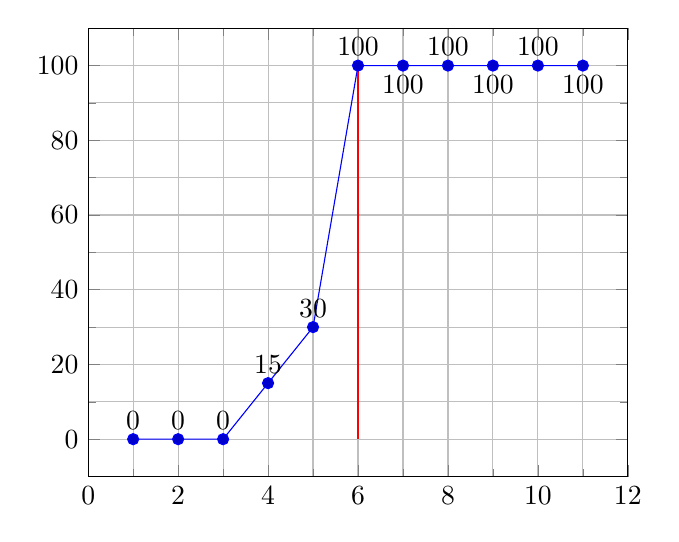
\begin{tikzpicture}
\begin{axis}[grid=both,minor tick num=1]
   \addplot coordinates
      {(1,0)(2,0)(3,0)(4,15)(5,30)(6,100)(7,100)(8,100)(9,100)(10,100)(11,100)};
   \node [above] at (axis cs: 1,0) {$0$};
   \node [above] at (axis cs: 2,0) {$0$};
   \node [above] at (axis cs: 3,0) {$0$};
   \node [above] at (axis cs: 4,15) {$15$};
   \node [above] at (axis cs: 5,30) {$30$};
   \node [above] at (axis cs: 6,100) {$100$};
   \node [below] at (axis cs: 7,100) {$100$};
   \node [above] at (axis cs: 8,100) {$100$};
   \node [below] at (axis cs: 9,100) {$100$};
   \node [above] at (axis cs: 10,100) {$100$};
   \node [below] at (axis cs: 11,100) {$100$};

   \addplot[red,sharp plot,update limits=false] coordinates
      {(6,0)(6,100)};
\end{axis}
\end{tikzpicture}
\end{adjustbox}
\end{center}
\caption[Gerechtigkeitseinschätzungen von Teilnehmer 1]{Gerechtigkeitseinschätzungen von Teilnehmer 1}
\end{figure}

\begin{figure}[H]
\begin{center}
\begin{adjustbox}{max width=0.25\textwidth}
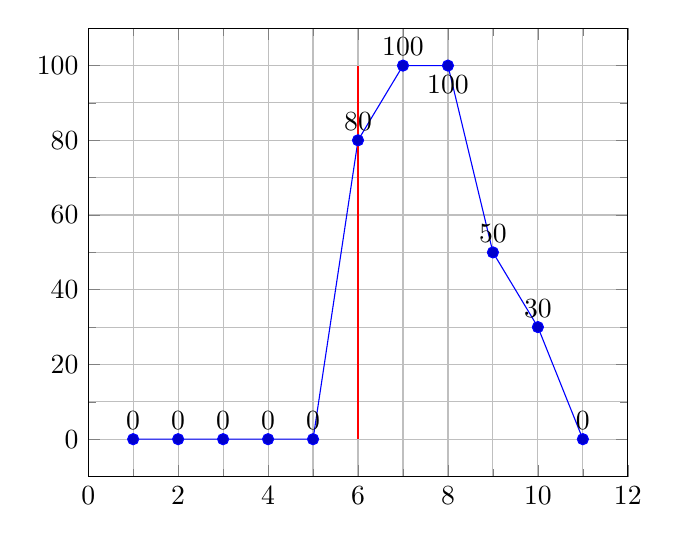
\begin{tikzpicture}
\begin{axis}[grid=both,minor tick num=1]
   \addplot coordinates
      {(1,0)(2,0)(3,0)(4,0)(5,0)(6,80)(7,100)(8,100)(9,50)(10,30)(11,0)};
   \node [above] at (axis cs: 1,0) {$0$};
   \node [above] at (axis cs: 2,0) {$0$};
   \node [above] at (axis cs: 3,0) {$0$};
   \node [above] at (axis cs: 4,0) {$0$};
   \node [above] at (axis cs: 5,0) {$0$};
   \node [above] at (axis cs: 6,80) {$80$};
   \node [above] at (axis cs: 7,100) {$100$};
   \node [below] at (axis cs: 8,100) {$100$};
   \node [above] at (axis cs: 9,50) {$50$};
   \node [above] at (axis cs: 10,30) {$30$};
   \node [above] at (axis cs: 11,0) {$0$};

   \addplot[red,sharp plot,update limits=false] coordinates
      {(6,0)(6,100)};
\end{axis}
\end{tikzpicture}
\end{adjustbox}
\end{center}
\caption[Gerechtigkeitseinschätzungen von Teilnehmer 2]{Gerechtigkeitseinschätzungen von Teilnehmer 2}
\end{figure}

\begin{figure}[H]
\begin{center}
\begin{adjustbox}{max width=0.25\textwidth}
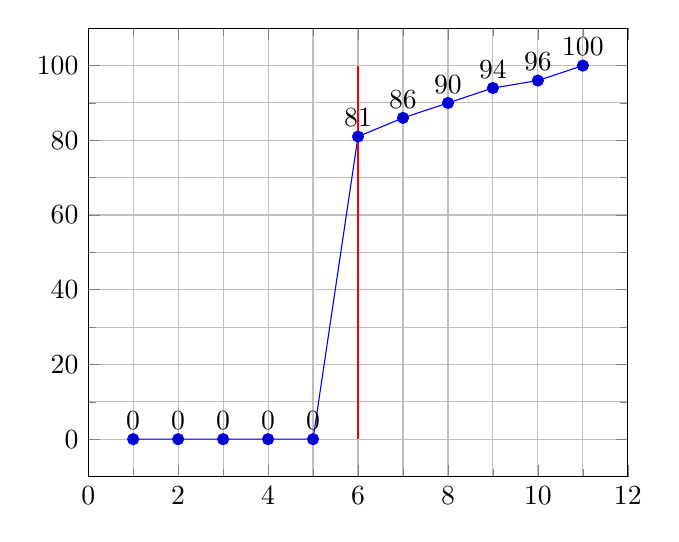
\begin{tikzpicture}
\begin{axis}[grid=both,minor tick num=1]
   \addplot coordinates
      {(1,0)(2,0)(3,0)(4,0)(5,0)(6,81)(7,86)(8,90)(9,94)(10,96)(11,100)};
   \node [above] at (axis cs: 1,0) {$0$};
   \node [above] at (axis cs: 2,0) {$0$};
   \node [above] at (axis cs: 3,0) {$0$};
   \node [above] at (axis cs: 4,0) {$0$};
   \node [above] at (axis cs: 5,0) {$0$};
   \node [above] at (axis cs: 6,81) {$81$};
   \node [above] at (axis cs: 7,86) {$86$};
   \node [above] at (axis cs: 8,90) {$90$};
   \node [above] at (axis cs: 9,94) {$94$};
   \node [above] at (axis cs: 10,96) {$96$};
   \node [above] at (axis cs: 11,100) {$100$};

   \addplot[red,sharp plot,update limits=false] coordinates
      {(6,0)(6,100)};
\end{axis}
\end{tikzpicture}
\end{adjustbox}
\end{center}
\caption[Gerechtigkeitseinschätzungen von Teilnehmer 3]{Gerechtigkeitseinschätzungen von Teilnehmer 3}
\end{figure}

\begin{figure}[H]
\begin{center}
\begin{adjustbox}{max width=0.25\textwidth}
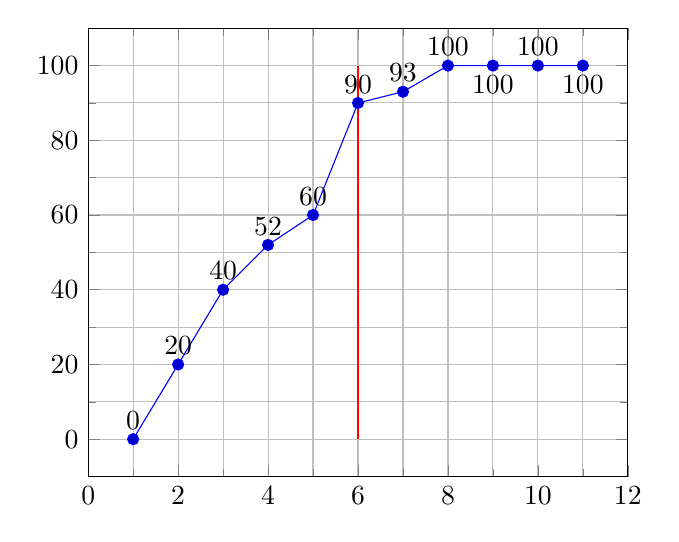
\begin{tikzpicture}
\begin{axis}[grid=both,minor tick num=1]
   \addplot coordinates
      {(1,0)(2,20)(3,40)(4,52)(5,60)(6,90)(7,93)(8,100)(9,100)(10,100)(11,100)};
   \node [above] at (axis cs: 1,0) {$0$};
   \node [above] at (axis cs: 2,20) {$20$};
   \node [above] at (axis cs: 3,40) {$40$};
   \node [above] at (axis cs: 4,52) {$52$};
   \node [above] at (axis cs: 5,60) {$60$};
   \node [above] at (axis cs: 6,90) {$90$};
   \node [above] at (axis cs: 7,93) {$93$};
   \node [above] at (axis cs: 8,100) {$100$};
   \node [below] at (axis cs: 9,100) {$100$};
   \node [above] at (axis cs: 10,100) {$100$};
   \node [below] at (axis cs: 11,100) {$100$};

   \addplot[red,sharp plot,update limits=false] coordinates
      {(6,0)(6,100)};
\end{axis}
\end{tikzpicture}
\end{adjustbox}
\end{center}
\caption[Gerechtigkeitseinschätzungen von Teilnehmer 4]{Gerechtigkeitseinschätzungen von Teilnehmer 4}
\end{figure}

\begin{figure}[H]
\begin{center}
\begin{adjustbox}{max width=0.25\textwidth}
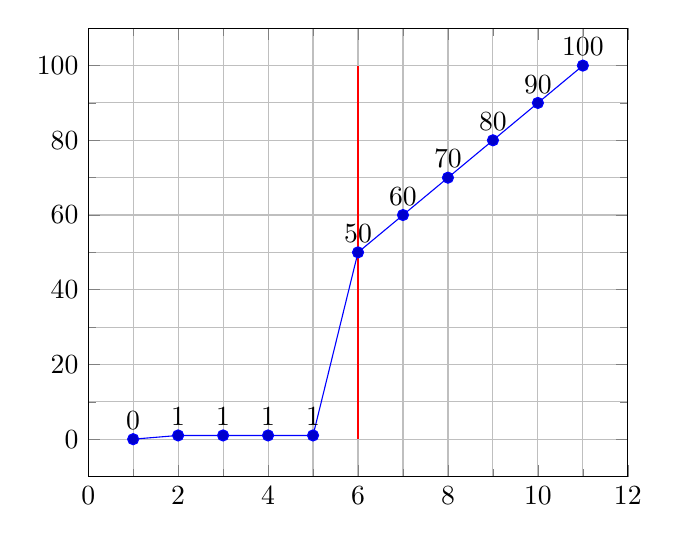
\begin{tikzpicture}
\begin{axis}[grid=both,minor tick num=1]
   \addplot coordinates
      {(1,0)(2,1)(3,1)(4,1)(5,1)(6,50)(7,60)(8,70)(9,80)(10,90)(11,100)};
   \node [above] at (axis cs: 1,0) {$0$};
   \node [above] at (axis cs: 2,1) {$1$};
   \node [above] at (axis cs: 3,1) {$1$};
   \node [above] at (axis cs: 4,1) {$1$};
   \node [above] at (axis cs: 5,1) {$1$};
   \node [above] at (axis cs: 6,50) {$50$};
   \node [above] at (axis cs: 7,60) {$60$};
   \node [above] at (axis cs: 8,70) {$70$};
   \node [above] at (axis cs: 9,80) {$80$};
   \node [above] at (axis cs: 10,90) {$90$};
   \node [above] at (axis cs: 11,100) {$100$};

   \addplot[red,sharp plot,update limits=false] coordinates
      {(6,0)(6,100)};
\end{axis}
\end{tikzpicture}
\end{adjustbox}
\end{center}
\caption[Gerechtigkeitseinschätzungen von Teilnehmer 5]{Gerechtigkeitseinschätzungen von Teilnehmer 5}
\end{figure}

\begin{figure}[H]
\begin{center}
\begin{adjustbox}{max width=0.25\textwidth}
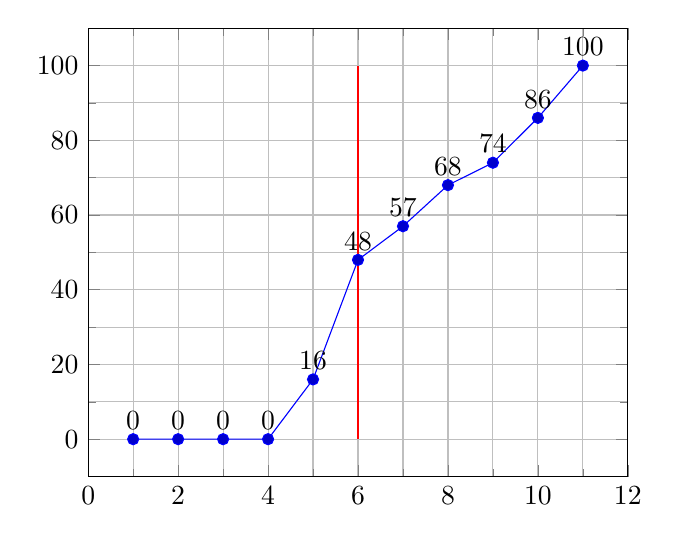
\begin{tikzpicture}
\begin{axis}[grid=both,minor tick num=1]
   \addplot coordinates
      {(1,0)(2,0)(3,0)(4,0)(5,16)(6,48)(7,57)(8,68)(9,74)(10,86)(11,100)};
   \node [above] at (axis cs: 1,0) {$0$};
   \node [above] at (axis cs: 2,0) {$0$};
   \node [above] at (axis cs: 3,0) {$0$};
   \node [above] at (axis cs: 4,0) {$0$};
   \node [above] at (axis cs: 5,16) {$16$};
   \node [above] at (axis cs: 6,48) {$48$};
   \node [above] at (axis cs: 7,57) {$57$};
   \node [above] at (axis cs: 8,68) {$68$};
   \node [above] at (axis cs: 9,74) {$74$};
   \node [above] at (axis cs: 10,86) {$86$};
   \node [above] at (axis cs: 11,100) {$100$};

   \addplot[red,sharp plot,update limits=false] coordinates
      {(6,0)(6,100)};
\end{axis}
\end{tikzpicture}
\end{adjustbox}
\end{center}
\caption[Gerechtigkeitseinschätzungen von Teilnehmer 6]{Gerechtigkeitseinschätzungen von Teilnehmer 6}
\end{figure}

\begin{figure}[H]
\begin{center}
\begin{adjustbox}{max width=0.25\textwidth}
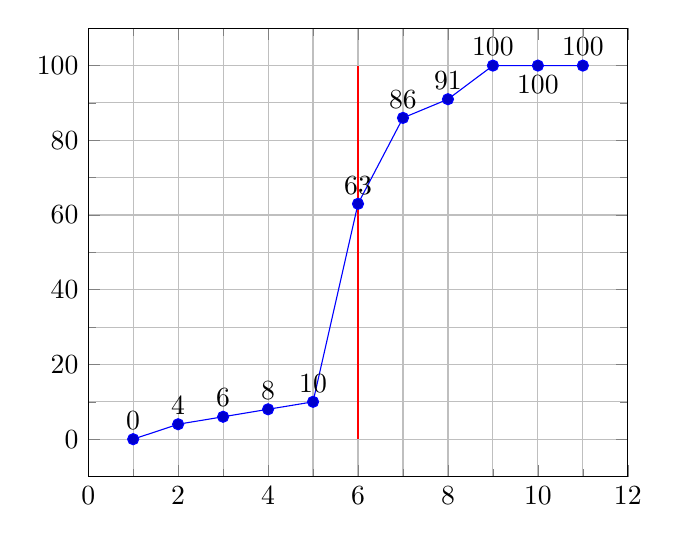
\begin{tikzpicture}
\begin{axis}[grid=both,minor tick num=1]
   \addplot coordinates
      {(1,0)(2,4)(3,6)(4,8)(5,10)(6,63)(7,86)(8,91)(9,100)(10,100)(11,100)};
   \node [above] at (axis cs: 1,0) {$0$};
   \node [above] at (axis cs: 2,4) {$4$};
   \node [above] at (axis cs: 3,6) {$6$};
   \node [above] at (axis cs: 4,8) {$8$};
   \node [above] at (axis cs: 5,10) {$10$};
   \node [above] at (axis cs: 6,63) {$63$};
   \node [above] at (axis cs: 7,86) {$86$};
   \node [above] at (axis cs: 8,91) {$91$};
   \node [above] at (axis cs: 9,100) {$100$};
   \node [below] at (axis cs: 10,100) {$100$};
   \node [above] at (axis cs: 11,100) {$100$};

   \addplot[red,sharp plot,update limits=false] coordinates
      {(6,0)(6,100)};
\end{axis}
\end{tikzpicture}
\end{adjustbox}
\end{center}
\caption[Gerechtigkeitseinschätzungen von Teilnehmer 7]{Gerechtigkeitseinschätzungen von Teilnehmer 7}
\end{figure}

\begin{figure}[H]
\begin{center}
\begin{adjustbox}{max width=0.25\textwidth}
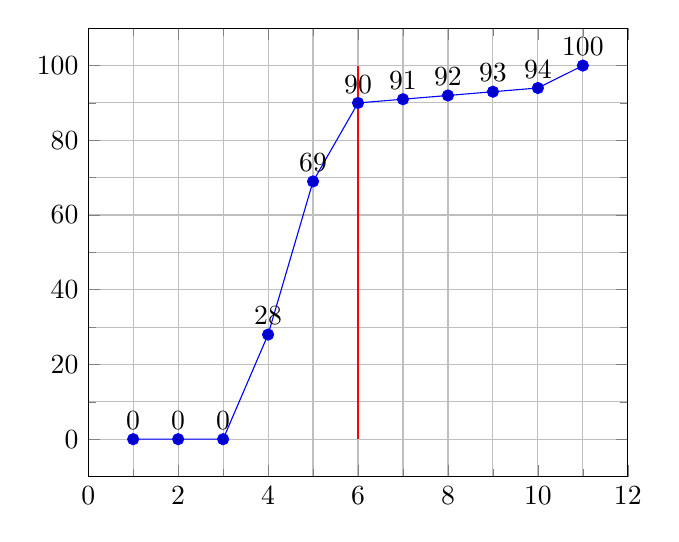
\begin{tikzpicture}
\begin{axis}[grid=both,minor tick num=1]
   \addplot coordinates
      {(1,0)(2,0)(3,0)(4,28)(5,69)(6,90)(7,91)(8,92)(9,93)(10,94)(11,100)};
   \node [above] at (axis cs: 1,0) {$0$};
   \node [above] at (axis cs: 2,0) {$0$};
   \node [above] at (axis cs: 3,0) {$0$};
   \node [above] at (axis cs: 4,28) {$28$};
   \node [above] at (axis cs: 5,69) {$69$};
   \node [above] at (axis cs: 6,90) {$90$};
   \node [above] at (axis cs: 7,91) {$91$};
   \node [above] at (axis cs: 8,92) {$92$};
   \node [above] at (axis cs: 9,93) {$93$};
   \node [above] at (axis cs: 10,94) {$94$};
   \node [above] at (axis cs: 11,100) {$100$};

   \addplot[red,sharp plot,update limits=false] coordinates
      {(6,0)(6,100)};
\end{axis}
\end{tikzpicture}
\end{adjustbox}
\end{center}
\caption[Gerechtigkeitseinschätzungen von Teilnehmer 8]{Gerechtigkeitseinschätzungen von Teilnehmer 8}
\end{figure}

\begin{figure}[H]
\begin{center}
\begin{adjustbox}{max width=0.25\textwidth}
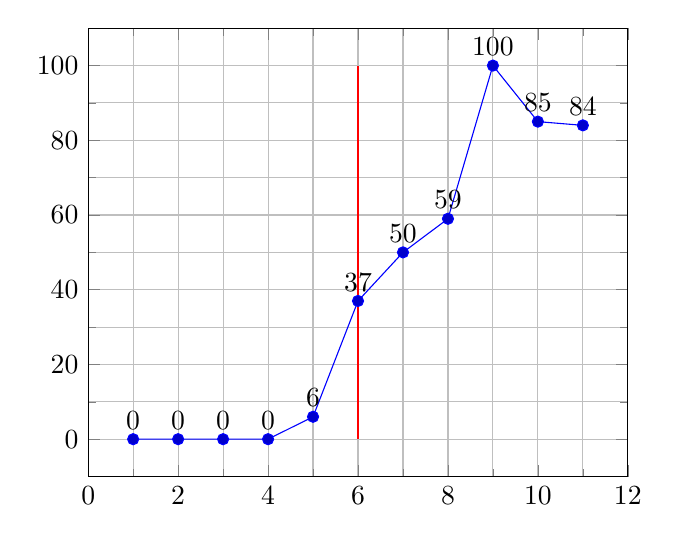
\begin{tikzpicture}
\begin{axis}[grid=both,minor tick num=1]
   \addplot coordinates
      {(1,0)(2,0)(3,0)(4,0)(5,6)(6,37)(7,50)(8,59)(9,100)(10,85)(11,84)};
   \node [above] at (axis cs: 1,0) {$0$};
   \node [above] at (axis cs: 2,0) {$0$};
   \node [above] at (axis cs: 3,0) {$0$};
   \node [above] at (axis cs: 4,0) {$0$};
   \node [above] at (axis cs: 5,6) {$6$};
   \node [above] at (axis cs: 6,37) {$37$};
   \node [above] at (axis cs: 7,50) {$50$};
   \node [above] at (axis cs: 8,59) {$59$};
   \node [above] at (axis cs: 9,100) {$100$};
   \node [above] at (axis cs: 10,85) {$85$};
   \node [above] at (axis cs: 11,84) {$84$};

   \addplot[red,sharp plot,update limits=false] coordinates
      {(6,0)(6,100)};
\end{axis}
\end{tikzpicture}
\end{adjustbox}
\end{center}
\caption[Gerechtigkeitseinschätzungen von Teilnehmer 9]{Gerechtigkeitseinschätzungen von Teilnehmer 9}
\end{figure}

\begin{figure}[H]
\begin{center}
\begin{adjustbox}{max width=0.25\textwidth}
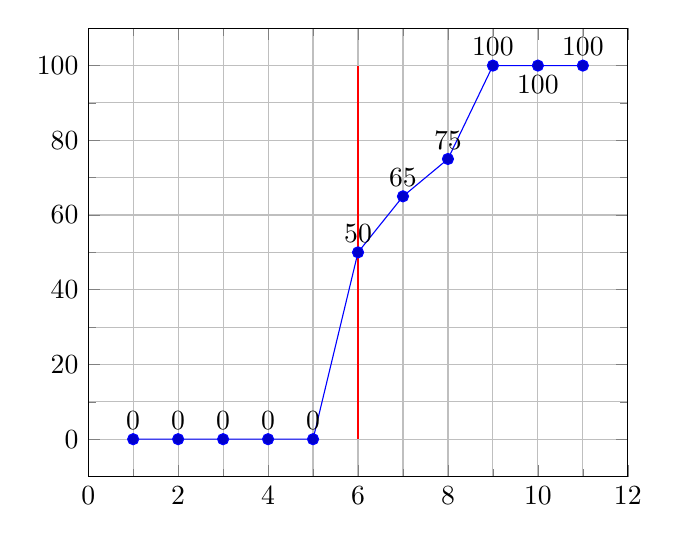
\begin{tikzpicture}
\begin{axis}[grid=both,minor tick num=1]
   \addplot coordinates
      {(1,0)(2,0)(3,0)(4,0)(5,0)(6,50)(7,65)(8,75)(9,100)(10,100)(11,100)};
   \node [above] at (axis cs: 1,0) {$0$};
   \node [above] at (axis cs: 2,0) {$0$};
   \node [above] at (axis cs: 3,0) {$0$};
   \node [above] at (axis cs: 4,0) {$0$};
   \node [above] at (axis cs: 5,0) {$0$};
   \node [above] at (axis cs: 6,50) {$50$};
   \node [above] at (axis cs: 7,65) {$65$};
   \node [above] at (axis cs: 8,75) {$75$};
   \node [above] at (axis cs: 9,100) {$100$};
   \node [below] at (axis cs: 10,100) {$100$};
   \node [above] at (axis cs: 11,100) {$100$};

   \addplot[red,sharp plot,update limits=false] coordinates
      {(6,0)(6,100)};
\end{axis}
\end{tikzpicture}
\end{adjustbox}
\end{center}
\caption[Gerechtigkeitseinschätzungen von Teilnehmer 10]{Gerechtigkeitseinschätzungen von Teilnehmer 10}
\end{figure}

\begin{figure}[H]
\begin{center}
\begin{adjustbox}{max width=0.25\textwidth}
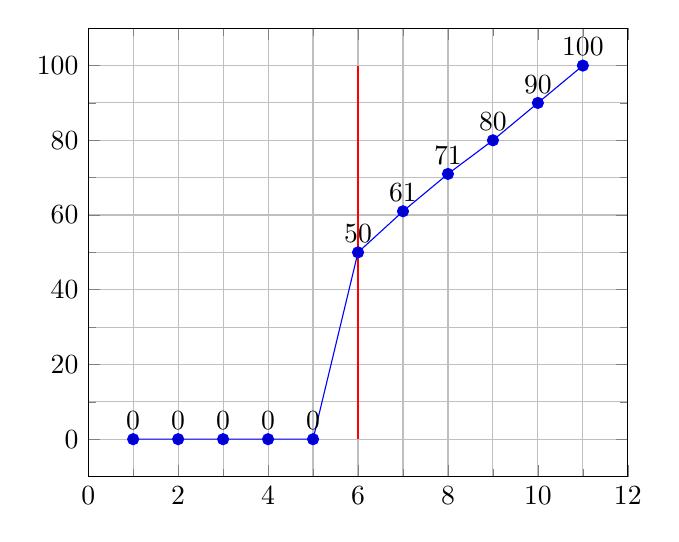
\begin{tikzpicture}
\begin{axis}[grid=both,minor tick num=1]
   \addplot coordinates
      {(1,0)(2,0)(3,0)(4,0)(5,0)(6,50)(7,61)(8,71)(9,80)(10,90)(11,100)};
   \node [above] at (axis cs: 1,0) {$0$};
   \node [above] at (axis cs: 2,0) {$0$};
   \node [above] at (axis cs: 3,0) {$0$};
   \node [above] at (axis cs: 4,0) {$0$};
   \node [above] at (axis cs: 5,0) {$0$};
   \node [above] at (axis cs: 6,50) {$50$};
   \node [above] at (axis cs: 7,61) {$61$};
   \node [above] at (axis cs: 8,71) {$71$};
   \node [above] at (axis cs: 9,80) {$80$};
   \node [above] at (axis cs: 10,90) {$90$};
   \node [above] at (axis cs: 11,100) {$100$};

   \addplot[red,sharp plot,update limits=false] coordinates
      {(6,0)(6,100)};
\end{axis}
\end{tikzpicture}
\end{adjustbox}
\end{center}
\caption[Gerechtigkeitseinschätzungen von Teilnehmer 11]{Gerechtigkeitseinschätzungen von Teilnehmer 11}
\end{figure}

\begin{figure}[H]
\begin{center}
\begin{adjustbox}{max width=0.25\textwidth}
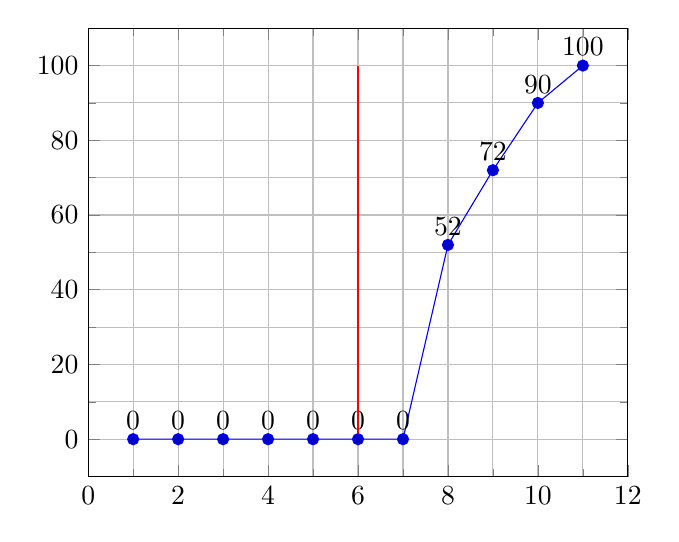
\begin{tikzpicture}
\begin{axis}[grid=both,minor tick num=1]
   \addplot coordinates
      {(1,0)(2,0)(3,0)(4,0)(5,0)(6,0)(7,0)(8,52)(9,72)(10,90)(11,100)};
   \node [above] at (axis cs: 1,0) {$0$};
   \node [above] at (axis cs: 2,0) {$0$};
   \node [above] at (axis cs: 3,0) {$0$};
   \node [above] at (axis cs: 4,0) {$0$};
   \node [above] at (axis cs: 5,0) {$0$};
   \node [above] at (axis cs: 6,0) {$0$};
   \node [above] at (axis cs: 7,0) {$0$};
   \node [above] at (axis cs: 8,52) {$52$};
   \node [above] at (axis cs: 9,72) {$72$};
   \node [above] at (axis cs: 10,90) {$90$};
   \node [above] at (axis cs: 11,100) {$100$};

   \addplot[red,sharp plot,update limits=false] coordinates
      {(6,0)(6,100)};
\end{axis}
\end{tikzpicture}
\end{adjustbox}
\end{center}
\caption[Gerechtigkeitseinschätzungen von Teilnehmer 12]{Gerechtigkeitseinschätzungen von Teilnehmer 12}
\end{figure}

\begin{figure}[H]
\begin{center}
\begin{adjustbox}{max width=0.25\textwidth}
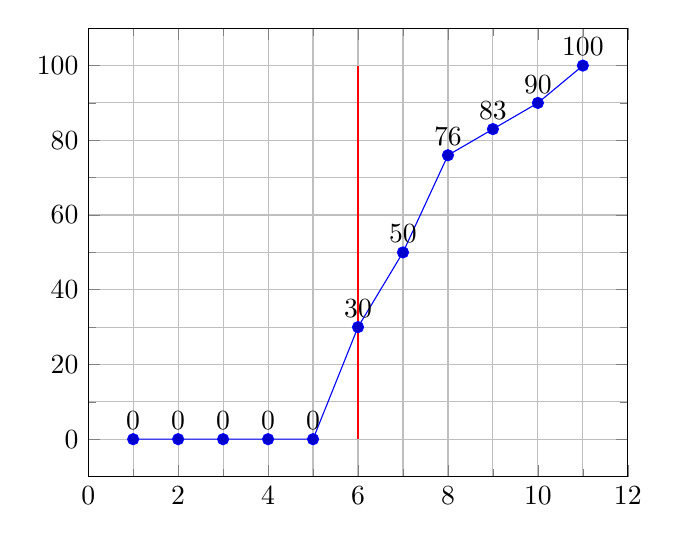
\begin{tikzpicture}
\begin{axis}[grid=both,minor tick num=1]
   \addplot coordinates
      {(1,0)(2,0)(3,0)(4,0)(5,0)(6,30)(7,50)(8,76)(9,83)(10,90)(11,100)};
   \node [above] at (axis cs: 1,0) {$0$};
   \node [above] at (axis cs: 2,0) {$0$};
   \node [above] at (axis cs: 3,0) {$0$};
   \node [above] at (axis cs: 4,0) {$0$};
   \node [above] at (axis cs: 5,0) {$0$};
   \node [above] at (axis cs: 6,30) {$30$};
   \node [above] at (axis cs: 7,50) {$50$};
   \node [above] at (axis cs: 8,76) {$76$};
   \node [above] at (axis cs: 9,83) {$83$};
   \node [above] at (axis cs: 10,90) {$90$};
   \node [above] at (axis cs: 11,100) {$100$};

   \addplot[red,sharp plot,update limits=false] coordinates
      {(6,0)(6,100)};
\end{axis}
\end{tikzpicture}
\end{adjustbox}
\end{center}
\caption[Gerechtigkeitseinschätzungen von Teilnehmer 13]{Gerechtigkeitseinschätzungen von Teilnehmer 13}
\end{figure}

\begin{figure}[H]
\begin{center}
\begin{adjustbox}{max width=0.25\textwidth}
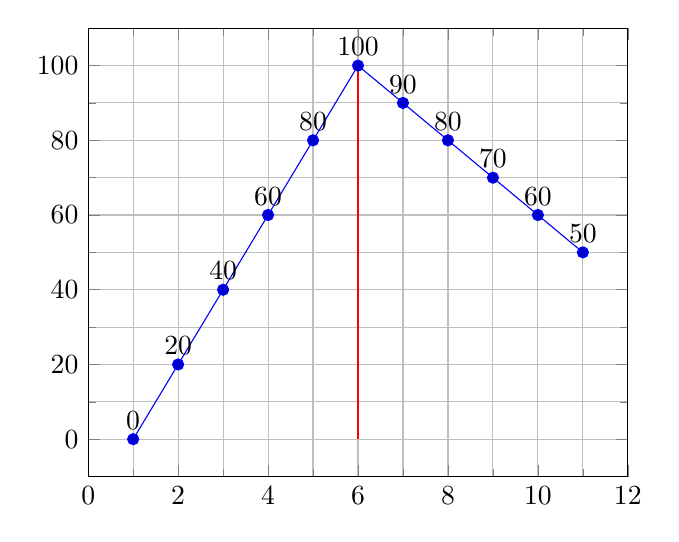
\begin{tikzpicture}
\begin{axis}[grid=both,minor tick num=1]
   \addplot coordinates
      {(1,0)(2,20)(3,40)(4,60)(5,80)(6,100)(7,90)(8,80)(9,70)(10,60)(11,50)};
   \node [above] at (axis cs: 1,0) {$0$};
   \node [above] at (axis cs: 2,20) {$20$};
   \node [above] at (axis cs: 3,40) {$40$};
   \node [above] at (axis cs: 4,60) {$60$};
   \node [above] at (axis cs: 5,80) {$80$};
   \node [above] at (axis cs: 6,100) {$100$};
   \node [above] at (axis cs: 7,90) {$90$};
   \node [above] at (axis cs: 8,80) {$80$};
   \node [above] at (axis cs: 9,70) {$70$};
   \node [above] at (axis cs: 10,60) {$60$};
   \node [above] at (axis cs: 11,50) {$50$};
	
   \addplot[red,sharp plot,update limits=false] coordinates
      {(6,0)(6,100)};
\end{axis}
\end{tikzpicture}
\end{adjustbox}
\end{center}
\caption[Gerechtigkeitseinschätzungen von Teilnehmer 14]{Gerechtigkeitseinschätzungen von Teilnehmer 14}
\end{figure}

\begin{figure}[H]
\begin{center}
\begin{adjustbox}{max width=0.25\textwidth}
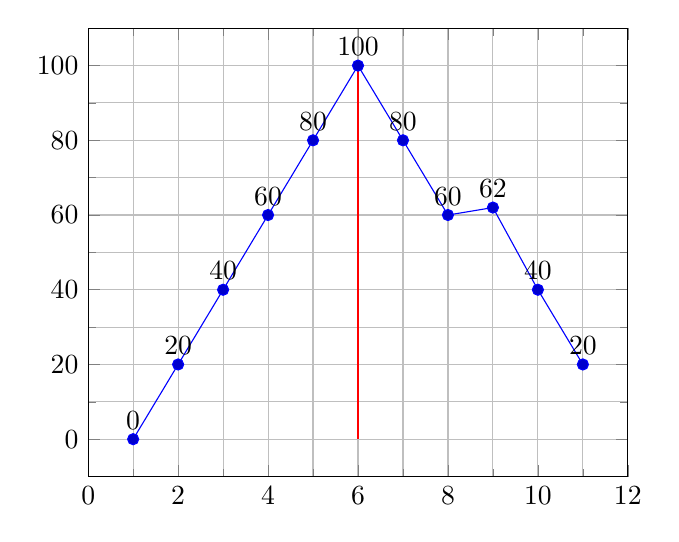
\begin{tikzpicture}
\begin{axis}[grid=both,minor tick num=1]
   \addplot coordinates
      {(1,0)(2,20)(3,40)(4,60)(5,80)(6,100)(7,80)(8,60)(9,62)(10,40)(11,20)};
   \node [above] at (axis cs: 1,0) {$0$};
   \node [above] at (axis cs: 2,20) {$20$};
   \node [above] at (axis cs: 3,40) {$40$};
   \node [above] at (axis cs: 4,60) {$60$};
   \node [above] at (axis cs: 5,80) {$80$};
   \node [above] at (axis cs: 6,100) {$100$};
   \node [above] at (axis cs: 7,80) {$80$};
   \node [above] at (axis cs: 8,60) {$60$};
   \node [above] at (axis cs: 9,62) {$62$};
   \node [above] at (axis cs: 10,40) {$40$};
   \node [above] at (axis cs: 11,20) {$20$};

   \addplot[red,sharp plot,update limits=false] coordinates
      {(6,0)(6,100)};
\end{axis}
\end{tikzpicture}
\end{adjustbox}
\end{center}
\caption[Gerechtigkeitseinschätzungen von Teilnehmer 15]{Gerechtigkeitseinschätzungen von Teilnehmer 15}
\end{figure}

\begin{figure}[H]
\begin{center}
\begin{adjustbox}{max width=0.25\textwidth}
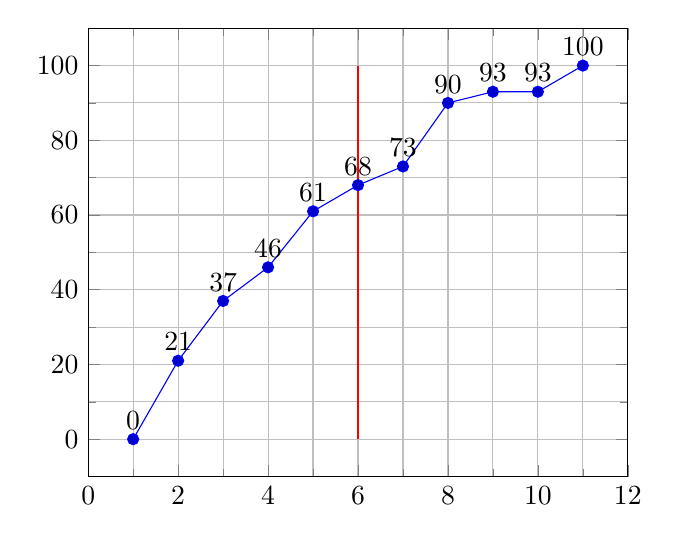
\begin{tikzpicture}
\begin{axis}[grid=both,minor tick num=1]
   \addplot coordinates
      {(1,0)(2,21)(3,37)(4,46)(5,61)(6,68)(7,73)(8,90)(9,93)(10,93)(11,100)};
   \node [above] at (axis cs: 1,0) {$0$};
   \node [above] at (axis cs: 2,21) {$21$};
   \node [above] at (axis cs: 3,37) {$37$};
   \node [above] at (axis cs: 4,46) {$46$};
   \node [above] at (axis cs: 5,61) {$61$};
   \node [above] at (axis cs: 6,68) {$68$};
   \node [above] at (axis cs: 7,73) {$73$};
   \node [above] at (axis cs: 8,90) {$90$};
   \node [above] at (axis cs: 9,93) {$93$};
   \node [above] at (axis cs: 10,93) {$93$};
   \node [above] at (axis cs: 11,100) {$100$};

   \addplot[red,sharp plot,update limits=false] coordinates
      {(6,0)(6,100)};
\end{axis}
\end{tikzpicture}
\end{adjustbox}
\end{center}
\caption[Gerechtigkeitseinschätzungen von Teilnehmer 16]{Gerechtigkeitseinschätzungen von Teilnehmer 16}
\end{figure}

\begin{figure}[H]
\begin{center}
\begin{adjustbox}{max width=0.25\textwidth}
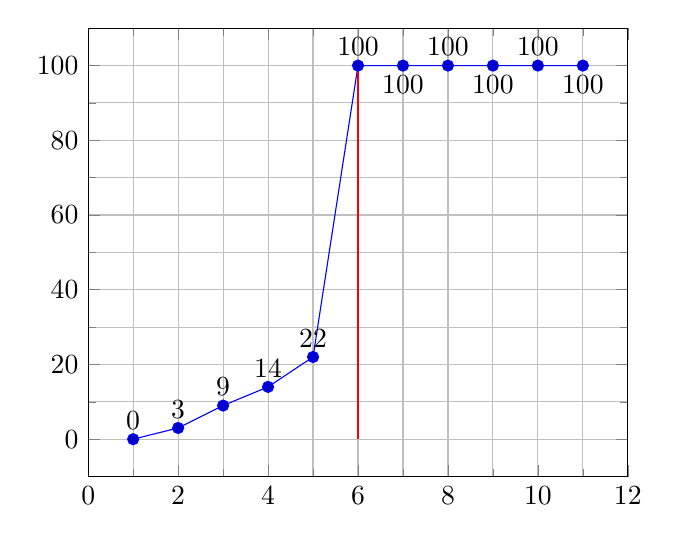
\begin{tikzpicture}
\begin{axis}[grid=both,minor tick num=1]
   \addplot coordinates
      {(1,0)(2,3)(3,9)(4,14)(5,22)(6,100)(7,100)(8,100)(9,100)(10,100)(11,100)};
   \node [above] at (axis cs: 1,0) {$0$};
   \node [above] at (axis cs: 2,3) {$3$};
   \node [above] at (axis cs: 3,9) {$9$};
   \node [above] at (axis cs: 4,14) {$14$};
   \node [above] at (axis cs: 5,22) {$22$};
   \node [above] at (axis cs: 6,100) {$100$};
   \node [below] at (axis cs: 7,100) {$100$};
   \node [above] at (axis cs: 8,100) {$100$};
   \node [below] at (axis cs: 9,100) {$100$};
   \node [above] at (axis cs: 10,100) {$100$};
   \node [below] at (axis cs: 11,100) {$100$};

   \addplot[red,sharp plot,update limits=false] coordinates
      {(6,0)(6,100)};
\end{axis}
\end{tikzpicture}
\end{adjustbox}
\end{center}
\caption[Gerechtigkeitseinschätzungen von Teilnehmer 17]{Gerechtigkeitseinschätzungen von Teilnehmer 17}
\end{figure}

\begin{figure}[H]
\begin{center}
\begin{adjustbox}{max width=0.25\textwidth}
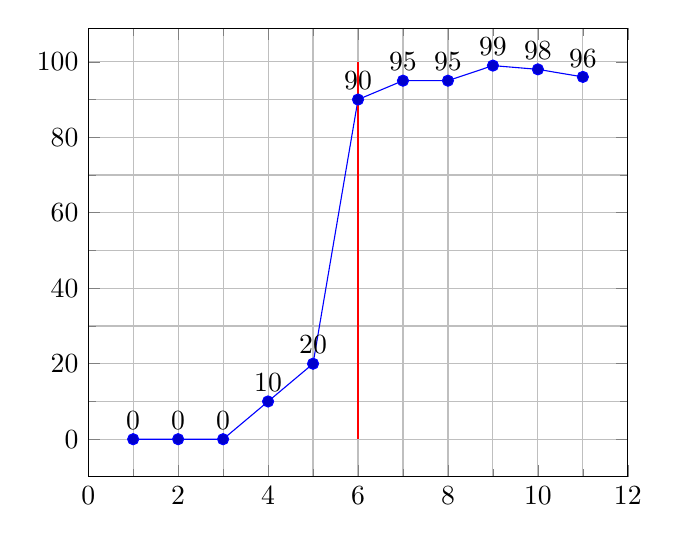
\begin{tikzpicture}
\begin{axis}[grid=both,minor tick num=1]
   \addplot coordinates
      {(1,0)(2,0)(3,0)(4,10)(5,20)(6,90)(7,95)(8,95)(9,99)(10,98)(11,96)};
   \node [above] at (axis cs: 1,0) {$0$};
   \node [above] at (axis cs: 2,0) {$0$};
   \node [above] at (axis cs: 3,0) {$0$};
   \node [above] at (axis cs: 4,10) {$10$};
   \node [above] at (axis cs: 5,20) {$20$};
   \node [above] at (axis cs: 6,90) {$90$};
   \node [above] at (axis cs: 7,95) {$95$};
   \node [above] at (axis cs: 8,95) {$95$};
   \node [above] at (axis cs: 9,99) {$99$};
   \node [above] at (axis cs: 10,98) {$98$};
   \node [above] at (axis cs: 11,96) {$96$};

   \addplot[red,sharp plot,update limits=false] coordinates
      {(6,0)(6,100)};
\end{axis}
\end{tikzpicture}
\end{adjustbox}
\end{center}
\caption[Gerechtigkeitseinschätzungen von Teilnehmer 18]{Gerechtigkeitseinschätzungen von Teilnehmer 18}
\end{figure}

\begin{figure}[H]
\begin{center}
\begin{adjustbox}{max width=0.25\textwidth}
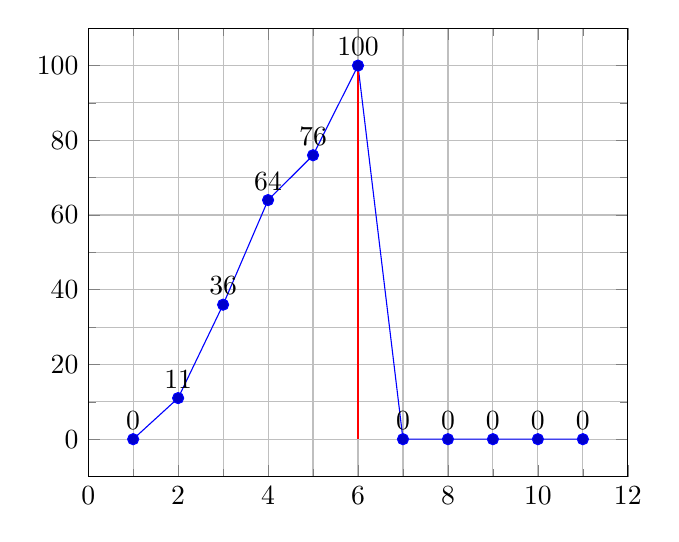
\begin{tikzpicture}
\begin{axis}[grid=both,minor tick num=1]
   \addplot coordinates
      {(1,0)(2,11)(3,36)(4,64)(5,76)(6,100)(7,0)(8,0)(9,0)(10,0)(11,0)};
   \node [above] at (axis cs: 1,0) {$0$};
   \node [above] at (axis cs: 2,11) {$11$};
   \node [above] at (axis cs: 3,36) {$36$};
   \node [above] at (axis cs: 4,64) {$64$};
   \node [above] at (axis cs: 5,76) {$76$};
   \node [above] at (axis cs: 6,100) {$100$};
   \node [above] at (axis cs: 7,0) {$0$};
   \node [above] at (axis cs: 8,0) {$0$};
   \node [above] at (axis cs: 9,0) {$0$};
   \node [above] at (axis cs: 10,0) {$0$};
   \node [above] at (axis cs: 11,0) {$0$};

   \addplot[red,sharp plot,update limits=false] coordinates
      {(6,0)(6,100)};
\end{axis}
\end{tikzpicture}
\end{adjustbox}
\end{center}
\caption[Gerechtigkeitseinschätzungen von Teilnehmer 19]{Gerechtigkeitseinschätzungen von Teilnehmer 19}
\end{figure}

\begin{figure}[H]
\begin{center}
\begin{adjustbox}{max width=0.25\textwidth}
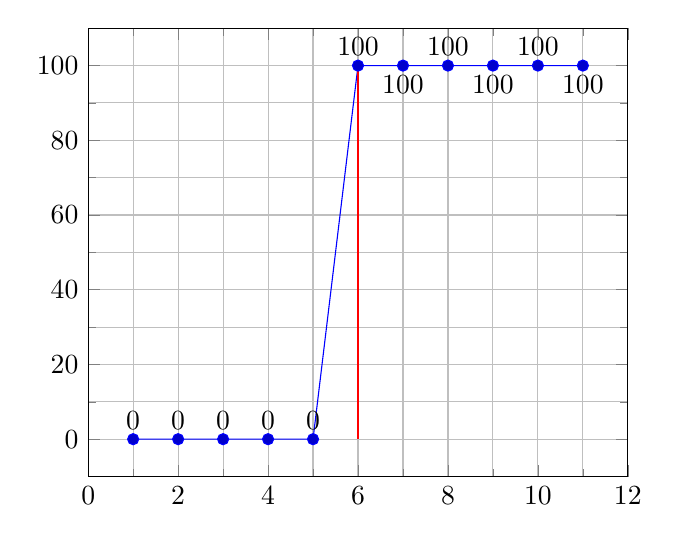
\begin{tikzpicture}
\begin{axis}[grid=both,minor tick num=1]
   \addplot coordinates
      {(1,0)(2,0)(3,0)(4,0)(5,0)(6,100)(7,100)(8,100)(9,100)(10,100)(11,100)};
   \node [above] at (axis cs: 1,0) {$0$};
   \node [above] at (axis cs: 2,0) {$0$};
   \node [above] at (axis cs: 3,0) {$0$};
   \node [above] at (axis cs: 4,0) {$0$};
   \node [above] at (axis cs: 5,0) {$0$};
   \node [above] at (axis cs: 6,100) {$100$};
   \node [below] at (axis cs: 7,100) {$100$};
   \node [above] at (axis cs: 8,100) {$100$};
   \node [below] at (axis cs: 9,100) {$100$};
   \node [above] at (axis cs: 10,100) {$100$};
   \node [below] at (axis cs: 11,100) {$100$};

   \addplot[red,sharp plot,update limits=false] coordinates
      {(6,0)(6,100)};
\end{axis}
\end{tikzpicture}
\end{adjustbox}
\end{center}
\caption[Gerechtigkeitseinschätzungen von Teilnehmer 20]{Gerechtigkeitseinschätzungen von Teilnehmer 20}
\end{figure}

\begin{figure}[H]
\begin{center}
\begin{adjustbox}{max width=0.25\textwidth}
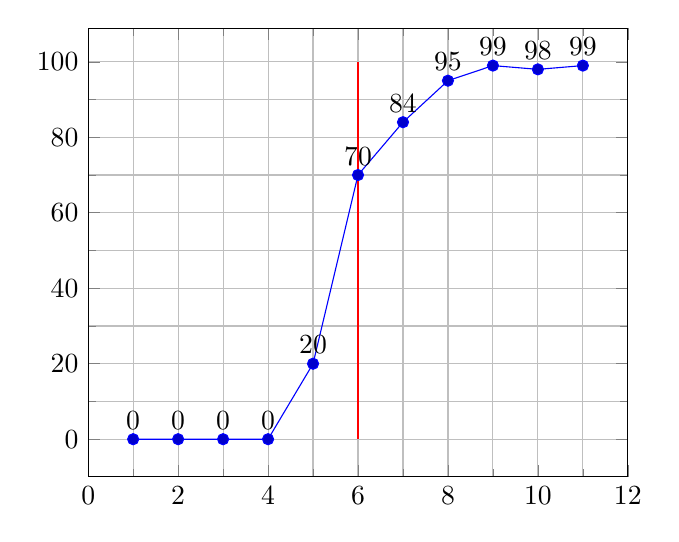
\begin{tikzpicture}
\begin{axis}[grid=both,minor tick num=1]
   \addplot coordinates
      {(1,0)(2,0)(3,0)(4,0)(5,20)(6,70)(7,84)(8,95)(9,99)(10,98)(11,99)};
   \node [above] at (axis cs: 1,0) {$0$};
   \node [above] at (axis cs: 2,0) {$0$};
   \node [above] at (axis cs: 3,0) {$0$};
   \node [above] at (axis cs: 4,0) {$0$};
   \node [above] at (axis cs: 5,20) {$20$};
   \node [above] at (axis cs: 6,70) {$70$};
   \node [above] at (axis cs: 7,84) {$84$};
   \node [above] at (axis cs: 8,95) {$95$};
   \node [above] at (axis cs: 9,99) {$99$};
   \node [above] at (axis cs: 10,98) {$98$};
   \node [above] at (axis cs: 11,99) {$99$};

   \addplot[red,sharp plot,update limits=false] coordinates
      {(6,0)(6,100)};
\end{axis}
\end{tikzpicture}
\end{adjustbox}
\end{center}
\caption[Gerechtigkeitseinschätzungen von Teilnehmer 21]{Gerechtigkeitseinschätzungen von Teilnehmer 21}
\end{figure}

\begin{figure}[H]
\begin{center}
\begin{adjustbox}{max width=0.25\textwidth}
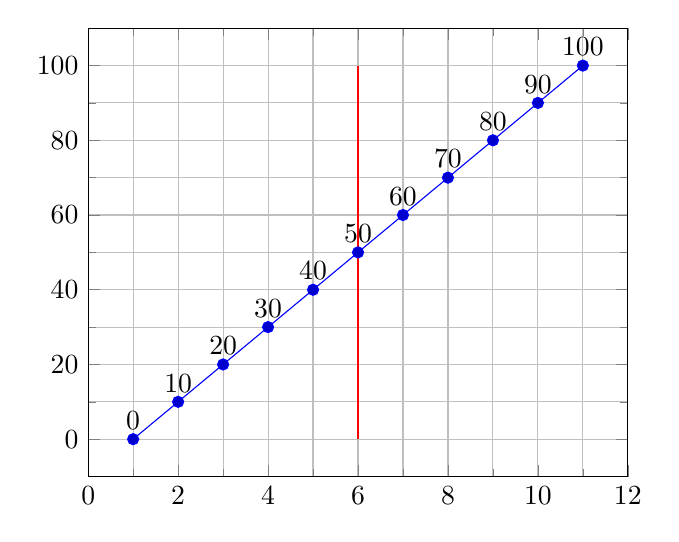
\begin{tikzpicture}
\begin{axis}[grid=both,minor tick num=1]
   \addplot coordinates
      {(1,0)(2,10)(3,20)(4,30)(5,40)(6,50)(7,60)(8,70)(9,80)(10,90)(11,100)};
   \node [above] at (axis cs: 1,0) {$0$};
   \node [above] at (axis cs: 2,10) {$10$};
   \node [above] at (axis cs: 3,20) {$20$};
   \node [above] at (axis cs: 4,30) {$30$};
   \node [above] at (axis cs: 5,40) {$40$};
   \node [above] at (axis cs: 6,50) {$50$};
   \node [above] at (axis cs: 7,60) {$60$};
   \node [above] at (axis cs: 8,70) {$70$};
   \node [above] at (axis cs: 9,80) {$80$};
   \node [above] at (axis cs: 10,90) {$90$};
   \node [above] at (axis cs: 11,100) {$100$};

   \addplot[red,sharp plot,update limits=false] coordinates
      {(6,0)(6,100)};
\end{axis}
\end{tikzpicture}
\end{adjustbox}
\end{center}
\caption[Gerechtigkeitseinschätzungen von Teilnehmer 22]{Gerechtigkeitseinschätzungen von Teilnehmer 22}
\end{figure}

\begin{figure}[H]
\begin{center}
\begin{adjustbox}{max width=0.25\textwidth}
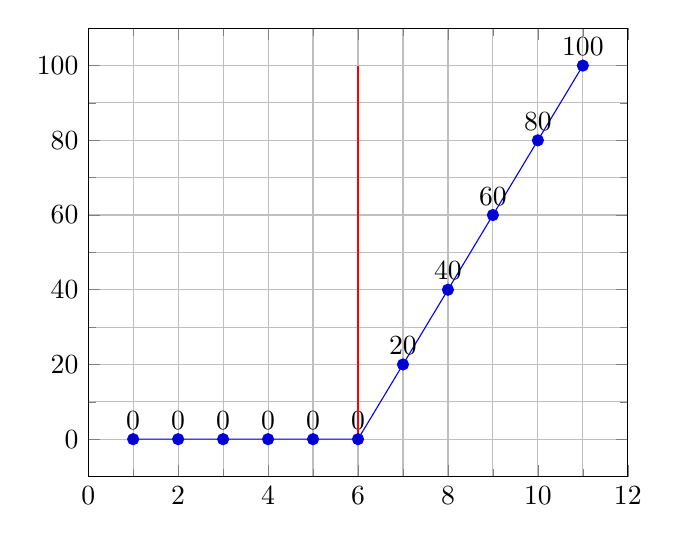
\begin{tikzpicture}
\begin{axis}[grid=both,minor tick num=1]
   \addplot coordinates
      {(1,0)(2,0)(3,0)(4,0)(5,0)(6,0)(7,20)(8,40)(9,60)(10,80)(11,100)};
   \node [above] at (axis cs: 1,0) {$0$};
   \node [above] at (axis cs: 2,0) {$0$};
   \node [above] at (axis cs: 3,0) {$0$};
   \node [above] at (axis cs: 4,0) {$0$};
   \node [above] at (axis cs: 5,0) {$0$};
   \node [above] at (axis cs: 6,0) {$0$};
   \node [above] at (axis cs: 7,20) {$20$};
   \node [above] at (axis cs: 8,40) {$40$};
   \node [above] at (axis cs: 9,60) {$60$};
   \node [above] at (axis cs: 10,80) {$80$};
   \node [above] at (axis cs: 11,100) {$100$};

   \addplot[red,sharp plot,update limits=false] coordinates
      {(6,0)(6,100)};
\end{axis}
\end{tikzpicture}
\end{adjustbox}
\end{center}
\caption[Gerechtigkeitseinschätzungen von Teilnehmer 23]{Gerechtigkeitseinschätzungen von Teilnehmer 23}
\end{figure}

\begin{figure}[H]
\begin{center}
\begin{adjustbox}{max width=0.25\textwidth}
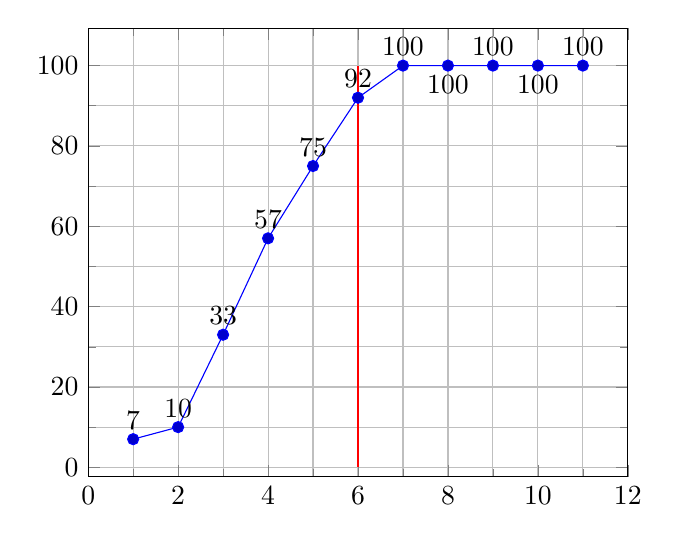
\begin{tikzpicture}
\begin{axis}[grid=both,minor tick num=1]
   \addplot coordinates
      {(1,7)(2,10)(3,33)(4,57)(5,75)(6,92)(7,100)(8,100)(9,100)(10,100)(11,100)};
   \node [above] at (axis cs: 1,7) {$7$};
   \node [above] at (axis cs: 2,10) {$10$};
   \node [above] at (axis cs: 3,33) {$33$};
   \node [above] at (axis cs: 4,57) {$57$};
   \node [above] at (axis cs: 5,75) {$75$};
   \node [above] at (axis cs: 6,92) {$92$};
   \node [above] at (axis cs: 7,100) {$100$};
   \node [below] at (axis cs: 8,100) {$100$};
   \node [above] at (axis cs: 9,100) {$100$};
   \node [below] at (axis cs: 10,100) {$100$};
   \node [above] at (axis cs: 11,100) {$100$};

   \addplot[red,sharp plot,update limits=false] coordinates
      {(6,0)(6,100)};
\end{axis}
\end{tikzpicture}
\end{adjustbox}
\end{center}
\caption[Gerechtigkeitseinschätzungen von Teilnehmer 24]{Gerechtigkeitseinschätzungen von Teilnehmer 24}
\end{figure}

\begin{figure}[H]
\begin{center}
\begin{adjustbox}{max width=0.25\textwidth}
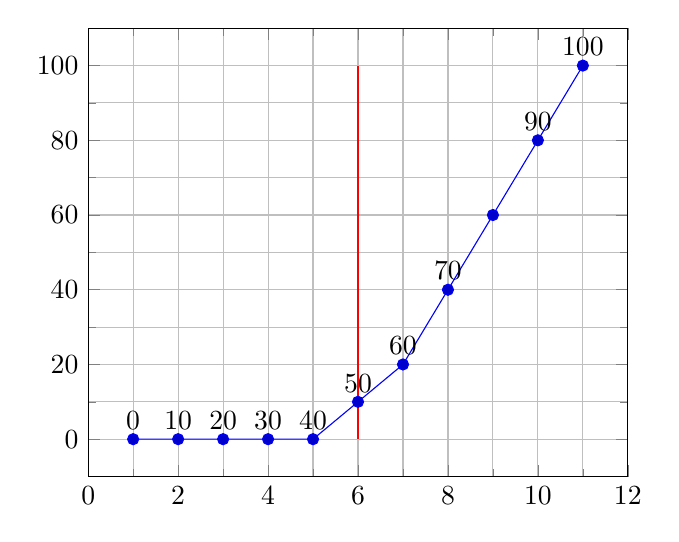
\begin{tikzpicture}
\begin{axis}[grid=both,minor tick num=1]
   \addplot coordinates
      {(1,0)(2,0)(3,0)(4,0)(5,0)(6,10)(7,20)(8,40)(9,60)(10,80)(11,100)};
   \node [above] at (axis cs: 1,0) {$0$};
   \node [above] at (axis cs: 2,0) {$10$};
   \node [above] at (axis cs: 3,0) {$20$};
   \node [above] at (axis cs: 4,0) {$30$};
   \node [above] at (axis cs: 5,0) {$40$};
   \node [above] at (axis cs: 6,10) {$50$};
   \node [above] at (axis cs: 7,20) {$60$};
   \node [above] at (axis cs: 8,40) {$70$};
   \node [above] at (axis cs: 9,600) {$80$};
   \node [above] at (axis cs: 10,80) {$90$};
   \node [above] at (axis cs: 11,100) {$100$};

   \addplot[red,sharp plot,update limits=false] coordinates
      {(6,0)(6,100)};
\end{axis}
\end{tikzpicture}
\end{adjustbox}
\end{center}
\caption[Gerechtigkeitseinschätzungen von Teilnehmer 25]{Gerechtigkeitseinschätzungen von Teilnehmer 25}
\end{figure}

\begin{figure}[H]
\begin{center}
\begin{adjustbox}{max width=0.25\textwidth}
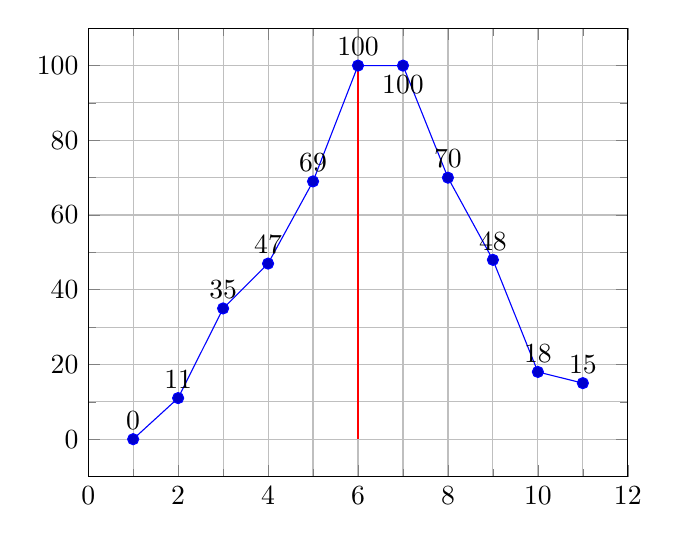
\begin{tikzpicture}
\begin{axis}[grid=both,minor tick num=1]
   \addplot coordinates
      {(1,0)(2,11)(3,35)(4,47)(5,69)(6,100)(7,100)(8,70)(9,48)(10,18)(11,15)};
   \node [above] at (axis cs: 1,0) {$0$};
   \node [above] at (axis cs: 2,11) {$11$};
   \node [above] at (axis cs: 3,35) {$35$};
   \node [above] at (axis cs: 4,47) {$47$};
   \node [above] at (axis cs: 5,69) {$69$};
   \node [above] at (axis cs: 6,100) {$100$};
   \node [below] at (axis cs: 7,100) {$100$};
   \node [above] at (axis cs: 8,70) {$70$};
   \node [above] at (axis cs: 9,48) {$48$};
   \node [above] at (axis cs: 10,18) {$18$};
   \node [above] at (axis cs: 11,15) {$15$};

   \addplot[red,sharp plot,update limits=false] coordinates
      {(6,0)(6,100)};
\end{axis}
\end{tikzpicture}
\end{adjustbox}
\end{center}
\caption[Gerechtigkeitseinschätzungen von Teilnehmer 26]{Gerechtigkeitseinschätzungen von Teilnehmer 26}
\end{figure}

\begin{figure}[H]
\begin{center}
\begin{adjustbox}{max width=0.25\textwidth}
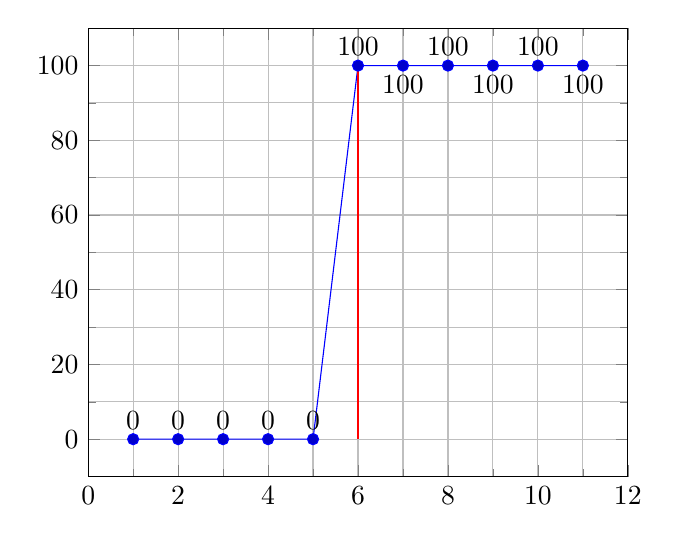
\begin{tikzpicture}
\begin{axis}[grid=both,minor tick num=1]
   \addplot coordinates
      {(1,0)(2,0)(3,0)(4,0)(5,0)(6,100)(7,100)(8,100)(9,100)(10,100)(11,100)};
   \node [above] at (axis cs: 1,0) {$0$};
   \node [above] at (axis cs: 2,0) {$0$};
   \node [above] at (axis cs: 3,0) {$0$};
   \node [above] at (axis cs: 4,0) {$0$};
   \node [above] at (axis cs: 5,0) {$0$};
   \node [above] at (axis cs: 6,100) {$100$};
   \node [below] at (axis cs: 7,100) {$100$};
   \node [above] at (axis cs: 8,100) {$100$};
   \node [below] at (axis cs: 9,100) {$100$};
   \node [above] at (axis cs: 10,100) {$100$};
   \node [below] at (axis cs: 11,100) {$100$};

   \addplot[red,sharp plot,update limits=false] coordinates
      {(6,0)(6,100)};
\end{axis}
\end{tikzpicture}
\end{adjustbox}
\end{center}
\caption[Gerechtigkeitseinschätzungen von Teilnehmer 27]{Gerechtigkeitseinschätzungen von Teilnehmer 27}
\end{figure}

\begin{figure}[H]
\begin{center}
\begin{adjustbox}{max width=0.25\textwidth}
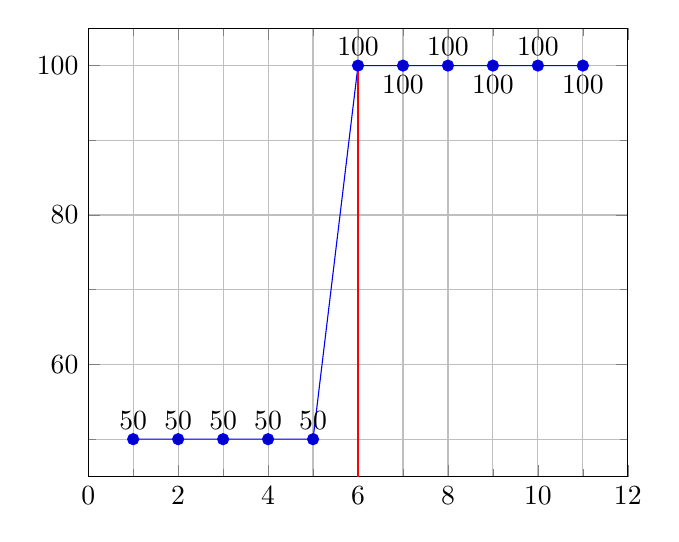
\begin{tikzpicture}
\begin{axis}[grid=both,minor tick num=1]
   \addplot coordinates
      {(1,50)(2,50)(3,50)(4,50)(5,50)(6,100)(7,100)(8,100)(9,100)(10,100)(11,100)};
   \node [above] at (axis cs: 1,50) {$50$};
   \node [above] at (axis cs: 2,50) {$50$};
   \node [above] at (axis cs: 3,50) {$50$};
   \node [above] at (axis cs: 4,50) {$50$};
   \node [above] at (axis cs: 5,50) {$50$};
   \node [above] at (axis cs: 6,100) {$100$};
   \node [below] at (axis cs: 7,100) {$100$};
   \node [above] at (axis cs: 8,100) {$100$};
   \node [below] at (axis cs: 9,100) {$100$};
   \node [above] at (axis cs: 10,100) {$100$};
   \node [below] at (axis cs: 11,100) {$100$};

   \addplot[red,sharp plot,update limits=false] coordinates
      {(6,0)(6,100)};
\end{axis}
\end{tikzpicture}
\end{adjustbox}
\end{center}
\caption[Gerechtigkeitseinschätzungen von Teilnehmer 28]{Gerechtigkeitseinschätzungen von Teilnehmer 28}
\end{figure}

\begin{figure}[H]
\begin{center}
\begin{adjustbox}{max width=0.25\textwidth}
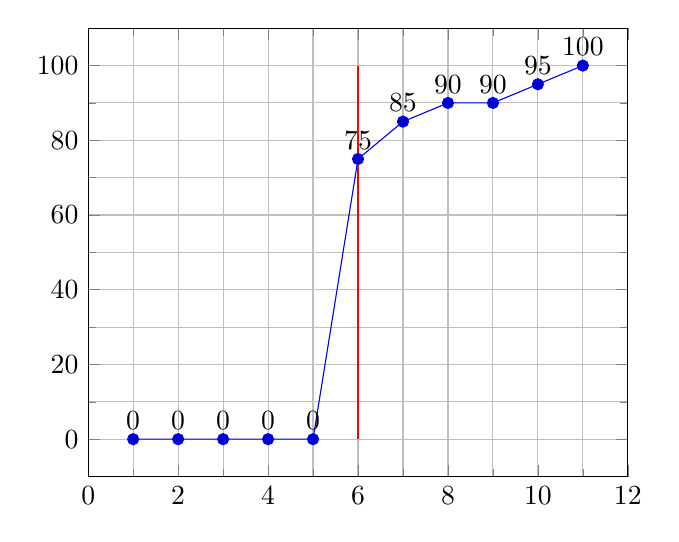
\begin{tikzpicture}
\begin{axis}[grid=both,minor tick num=1]
   \addplot coordinates
      {(1,0)(2,0)(3,0)(4,0)(5,0)(6,75)(7,85)(8,90)(9,90)(10,95)(11,100)};
   \node [above] at (axis cs: 1,0) {$0$};
   \node [above] at (axis cs: 2,0) {$0$};
   \node [above] at (axis cs: 3,0) {$0$};
   \node [above] at (axis cs: 4,0) {$0$};
   \node [above] at (axis cs: 5,0) {$0$};
   \node [above] at (axis cs: 6,75) {$75$};
   \node [above] at (axis cs: 7,85) {$85$};
   \node [above] at (axis cs: 8,90) {$90$};
   \node [above] at (axis cs: 9,90) {$90$};
   \node [above] at (axis cs: 10,95) {$95$};
   \node [above] at (axis cs: 11,100) {$100$};

   \addplot[red,sharp plot,update limits=false] coordinates
      {(6,0)(6,100)};
\end{axis}
\end{tikzpicture}
\end{adjustbox}
\end{center}
\caption[Gerechtigkeitseinschätzungen von Teilnehmer 29]{Gerechtigkeitseinschätzungen von Teilnehmer 29}
\end{figure}

\begin{figure}[H]
\begin{center}
\begin{adjustbox}{max width=0.25\textwidth}
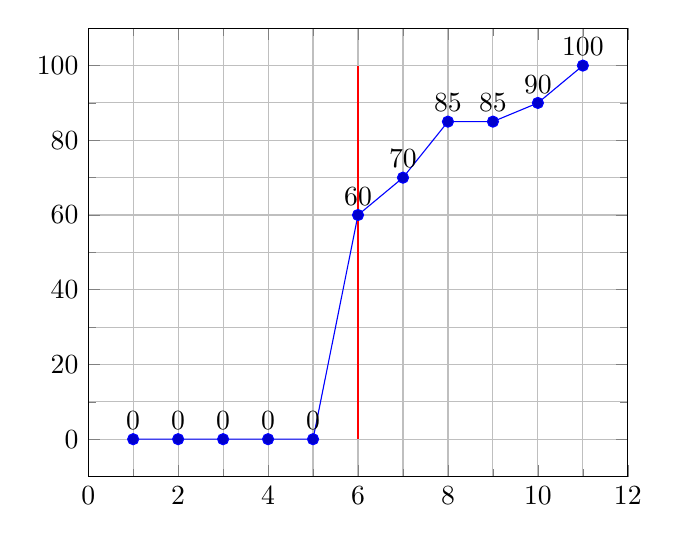
\begin{tikzpicture}
\begin{axis}[grid=both,minor tick num=1]
   \addplot coordinates
      {(1,0)(2,0)(3,0)(4,0)(5,0)(6,60)(7,70)(8,85)(9,85)(10,90)(11,100)};
   \node [above] at (axis cs: 1,0) {$0$};
   \node [above] at (axis cs: 2,0) {$0$};
   \node [above] at (axis cs: 3,0) {$0$};
   \node [above] at (axis cs: 4,0) {$0$};
   \node [above] at (axis cs: 5,0) {$0$};
   \node [above] at (axis cs: 6,60) {$60$};
   \node [above] at (axis cs: 7,70) {$70$};
   \node [above] at (axis cs: 8,85) {$85$};
   \node [above] at (axis cs: 9,85) {$85$};
   \node [above] at (axis cs: 10,90) {$90$};
   \node [above] at (axis cs: 11,100) {$100$};

   \addplot[red,sharp plot,update limits=false] coordinates
      {(6,0)(6,100)};
\end{axis}
\end{tikzpicture}
\end{adjustbox}
\end{center}
\caption[Gerechtigkeitseinschätzungen von Teilnehmer 30]{Gerechtigkeitseinschätzungen von Teilnehmer 30}
\end{figure}

\begin{figure}[H]
\begin{center}
\begin{adjustbox}{max width=0.25\textwidth}
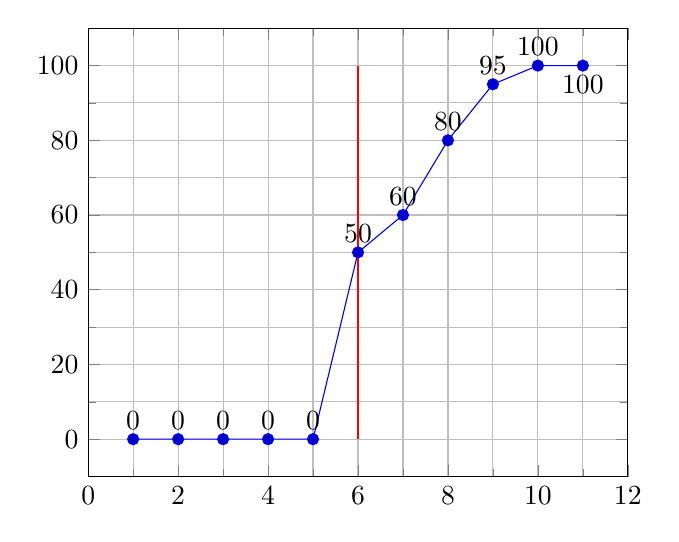
\begin{tikzpicture}
\begin{axis}[grid=both,minor tick num=1]
   \addplot coordinates
      {(1,0)(2,0)(3,0)(4,0)(5,0)(6,50)(7,60)(8,80)(9,95)(10,100)(11,100)};
   \node [above] at (axis cs: 1,0) {$0$};
   \node [above] at (axis cs: 2,0) {$0$};
   \node [above] at (axis cs: 3,0) {$0$};
   \node [above] at (axis cs: 4,0) {$0$};
   \node [above] at (axis cs: 5,0) {$0$};
   \node [above] at (axis cs: 6,50) {$50$};
   \node [above] at (axis cs: 7,60) {$60$};
   \node [above] at (axis cs: 8,80) {$80$};
   \node [above] at (axis cs: 9,95) {$95$};
   \node [above] at (axis cs: 10,100) {$100$};
   \node [below] at (axis cs: 11,100) {$100$};

   \addplot[red,sharp plot,update limits=false] coordinates
      {(6,0)(6,100)};
\end{axis}
\end{tikzpicture}
\end{adjustbox}
\end{center}
\caption[Gerechtigkeitseinschätzungen von Teilnehmer 31]{Gerechtigkeitseinschätzungen von Teilnehmer 31}
\end{figure}

\begin{figure}[H]
\begin{center}
\begin{adjustbox}{max width=0.25\textwidth}
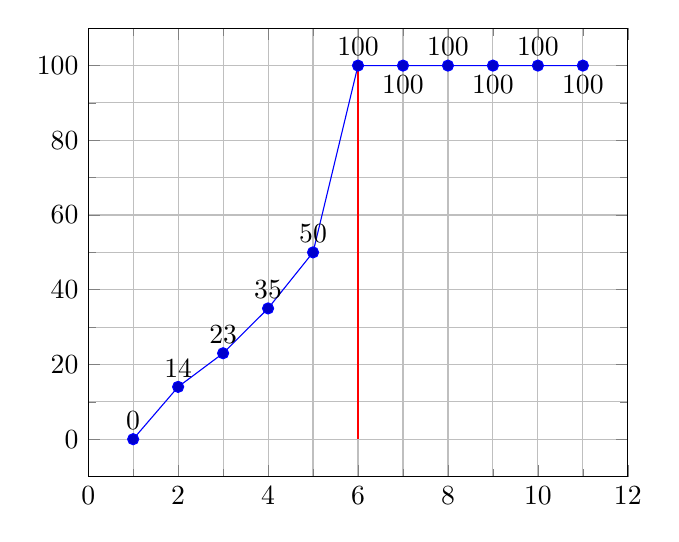
\begin{tikzpicture}
\begin{axis}[grid=both,minor tick num=1]
   \addplot coordinates
      {(1,0)(2,14)(3,23)(4,35)(5,50)(6,100)(7,100)(8,100)(9,100)(10,100)(11,100)};
   \node [above] at (axis cs: 1,0) {$0$};
   \node [above] at (axis cs: 2,14) {$14$};
   \node [above] at (axis cs: 3,23) {$23$};
   \node [above] at (axis cs: 4,35) {$35$};
   \node [above] at (axis cs: 5,50) {$50$};
   \node [above] at (axis cs: 6,100) {$100$};
   \node [below] at (axis cs: 7,100) {$100$};
   \node [above] at (axis cs: 8,100) {$100$};
   \node [below] at (axis cs: 9,100) {$100$};
   \node [above] at (axis cs: 10,100) {$100$};
   \node [below] at (axis cs: 11,100) {$100$};

   \addplot[red,sharp plot,update limits=false] coordinates
      {(6,0)(6,100)};
\end{axis}
\end{tikzpicture}
\end{adjustbox}
\end{center}
\caption[Gerechtigkeitseinschätzungen von Teilnehmer 32]{Gerechtigkeitseinschätzungen von Teilnehmer 32}
\end{figure}

\begin{figure}[H]
\begin{center}
\begin{adjustbox}{max width=0.25\textwidth}
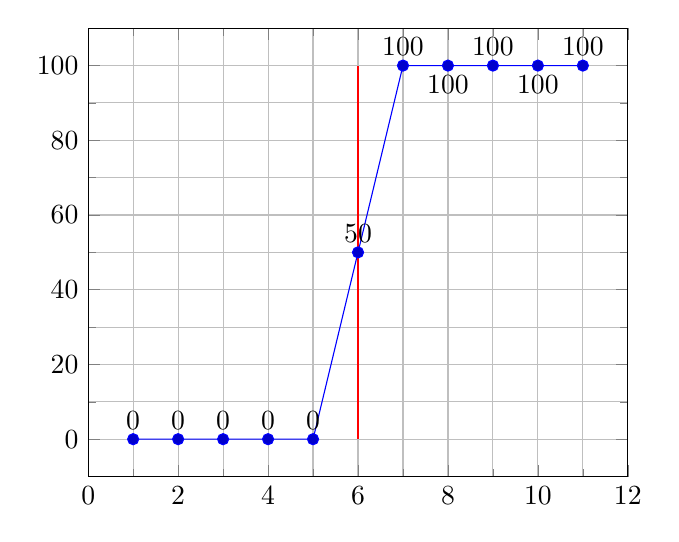
\begin{tikzpicture}
\begin{axis}[grid=both,minor tick num=1]
   \addplot coordinates
      {(1,0)(2,0)(3,0)(4,0)(5,0)(6,50)(7,100)(8,100)(9,100)(10,100)(11,100)};
   \node [above] at (axis cs: 1,0) {$0$};
   \node [above] at (axis cs: 2,0) {$0$};
   \node [above] at (axis cs: 3,0) {$0$};
   \node [above] at (axis cs: 4,0) {$0$};
   \node [above] at (axis cs: 5,0) {$0$};
   \node [above] at (axis cs: 6,50) {$50$};
   \node [above] at (axis cs: 7,100) {$100$};
   \node [below] at (axis cs: 8,100) {$100$};
   \node [above] at (axis cs: 9,100) {$100$};
   \node [below] at (axis cs: 10,100) {$100$};
   \node [above] at (axis cs: 11,100) {$100$};
	
   \addplot[red,sharp plot,update limits=false] coordinates
      {(6,0)(6,100)};
\end{axis}
\end{tikzpicture}
\end{adjustbox}
\end{center}
\caption[Gerechtigkeitseinschätzungen von Teilnehmer 33]{Gerechtigkeitseinschätzungen von Teilnehmer 33}
\end{figure}

\begin{figure}[H]
\begin{center}
\begin{adjustbox}{max width=0.25\textwidth}
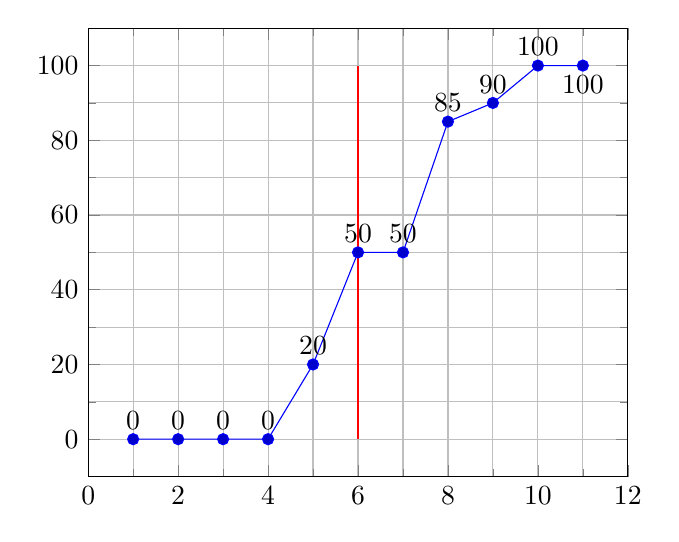
\begin{tikzpicture}
\begin{axis}[grid=both,minor tick num=1]
   \addplot coordinates
      {(1,0)(2,0)(3,0)(4,0)(5,20)(6,50)(7,50)(8,85)(9,90)(10,100)(11,100)};
   \node [above] at (axis cs: 1,0) {$0$};
   \node [above] at (axis cs: 2,0) {$0$};
   \node [above] at (axis cs: 3,0) {$0$};
   \node [above] at (axis cs: 4,0) {$0$};
   \node [above] at (axis cs: 5,20) {$20$};
   \node [above] at (axis cs: 6,50) {$50$};
   \node [above] at (axis cs: 7,50) {$50$};
   \node [above] at (axis cs: 8,85) {$85$};
   \node [above] at (axis cs: 9,90) {$90$};
   \node [above] at (axis cs: 10,100) {$100$};
   \node [below] at (axis cs: 11,100) {$100$};

   \addplot[red,sharp plot,update limits=false] coordinates
      {(6,0)(6,100)};
\end{axis}
\end{tikzpicture}
\end{adjustbox}
\end{center}
\caption[Gerechtigkeitseinschätzungen von Teilnehmer 34]{Gerechtigkeitseinschätzungen von Teilnehmer 34}
\end{figure}

\begin{figure}[H]
\begin{center}
\begin{adjustbox}{max width=0.25\textwidth}
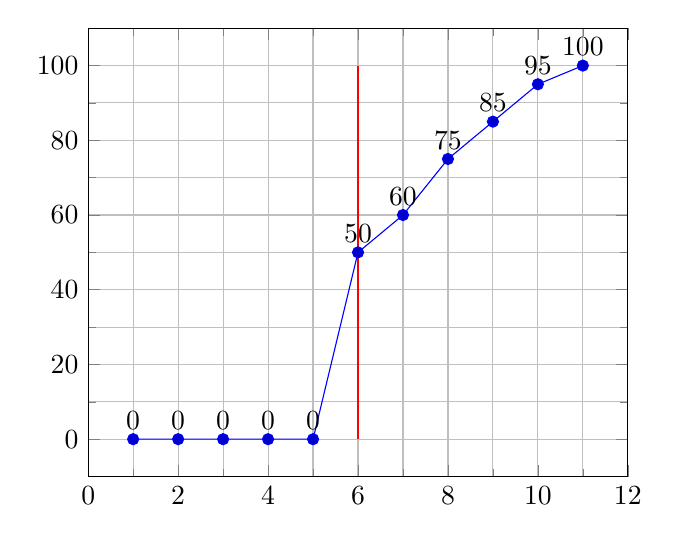
\begin{tikzpicture}
\begin{axis}[grid=both,minor tick num=1]
   \addplot coordinates
      {(1,0)(2,0)(3,0)(4,0)(5,0)(6,50)(7,60)(8,75)(9,85)(10,95)(11,100)};
   \node [above] at (axis cs: 1,0) {$0$};
   \node [above] at (axis cs: 2,0) {$0$};
   \node [above] at (axis cs: 3,0) {$0$};
   \node [above] at (axis cs: 4,0) {$0$};
   \node [above] at (axis cs: 5,0) {$0$};
   \node [above] at (axis cs: 6,50) {$50$};
   \node [above] at (axis cs: 7,60) {$60$};
   \node [above] at (axis cs: 8,75) {$75$};
   \node [above] at (axis cs: 9,85) {$85$};
   \node [above] at (axis cs: 10,95) {$95$};
   \node [above] at (axis cs: 11,100) {$100$};

   \addplot[red,sharp plot,update limits=false] coordinates
      {(6,0)(6,100)};
\end{axis}
\end{tikzpicture}
\end{adjustbox}
\end{center}
\caption[Gerechtigkeitseinschätzungen von Teilnehmer 35]{Gerechtigkeitseinschätzungen von Teilnehmer 35}
\end{figure}

\begin{figure}[H]
\begin{center}
\begin{adjustbox}{max width=0.25\textwidth}
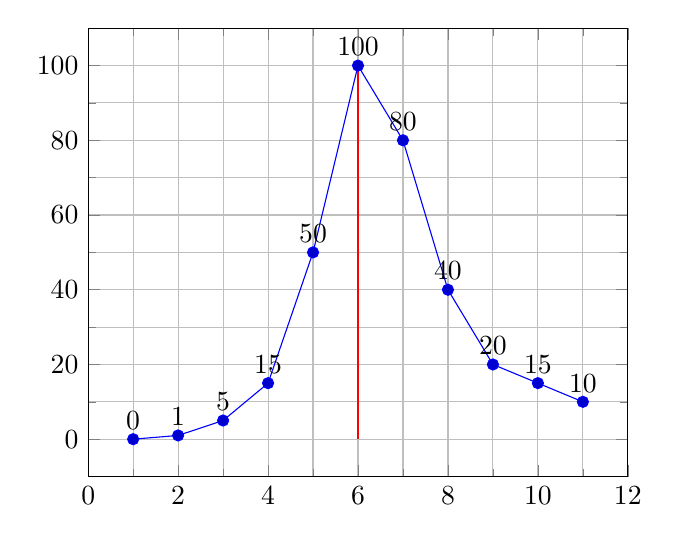
\begin{tikzpicture}
\begin{axis}[grid=both,minor tick num=1]
   \addplot coordinates
      {(1,0)(2,1)(3,5)(4,15)(5,50)(6,100)(7,80)(8,40)(9,20)(10,15)(11,10)};
   \node [above] at (axis cs: 1,0) {$0$};
   \node [above] at (axis cs: 2,1) {$1$};
   \node [above] at (axis cs: 3,5) {$5$};
   \node [above] at (axis cs: 4,15) {$15$};
   \node [above] at (axis cs: 5,50) {$50$};
   \node [above] at (axis cs: 6,100) {$100$};
   \node [above] at (axis cs: 7,80) {$80$};
   \node [above] at (axis cs: 8,40) {$40$};
   \node [above] at (axis cs: 9,20) {$20$};
   \node [above] at (axis cs: 10,15) {$15$};
   \node [above] at (axis cs: 11,10) {$10$};

   \addplot[red,sharp plot,update limits=false] coordinates
      {(6,0)(6,100)};
\end{axis}
\end{tikzpicture}
\end{adjustbox}
\end{center}
\caption[Gerechtigkeitseinschätzungen von Teilnehmer 36]{Gerechtigkeitseinschätzungen von Teilnehmer 36}
\end{figure}

\begin{figure}[H]
\begin{center}
\begin{adjustbox}{max width=0.25\textwidth}
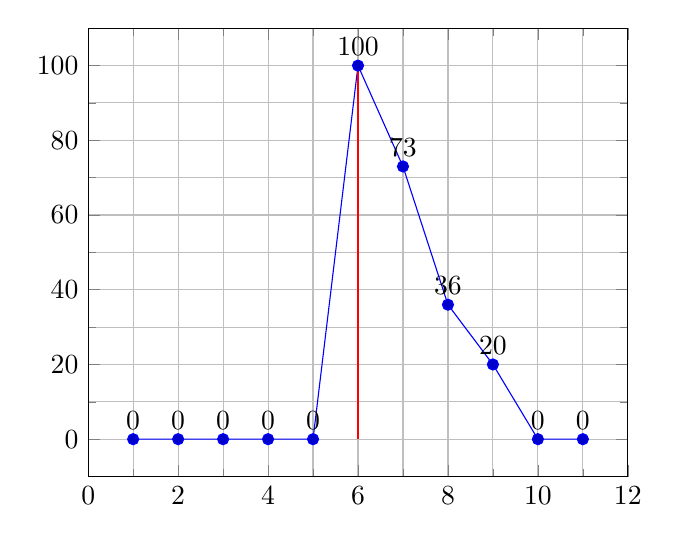
\begin{tikzpicture}
\begin{axis}[grid=both,minor tick num=1]
   \addplot coordinates
      {(1,0)(2,0)(3,0)(4,0)(5,0)(6,100)(7,73)(8,36)(9,20)(10,0)(11,0)};
   \node [above] at (axis cs: 1,0) {$0$};
   \node [above] at (axis cs: 2,0) {$0$};
   \node [above] at (axis cs: 3,0) {$0$};
   \node [above] at (axis cs: 4,0) {$0$};
   \node [above] at (axis cs: 5,0) {$0$};
   \node [above] at (axis cs: 6,100) {$100$};
   \node [above] at (axis cs: 7,73) {$73$};
   \node [above] at (axis cs: 8,36) {$36$};
   \node [above] at (axis cs: 9,20) {$20$};
   \node [above] at (axis cs: 10,0) {$0$};
   \node [above] at (axis cs: 11,0) {$0$};

   \addplot[red,sharp plot,update limits=false] coordinates
      {(6,0)(6,100)};
\end{axis}
\end{tikzpicture}
\end{adjustbox}
\end{center}
\caption[Gerechtigkeitseinschätzungen von Teilnehmer 37]{Gerechtigkeitseinschätzungen von Teilnehmer 37}
\end{figure}

\begin{figure}[H]
\begin{center}
\begin{adjustbox}{max width=0.25\textwidth}
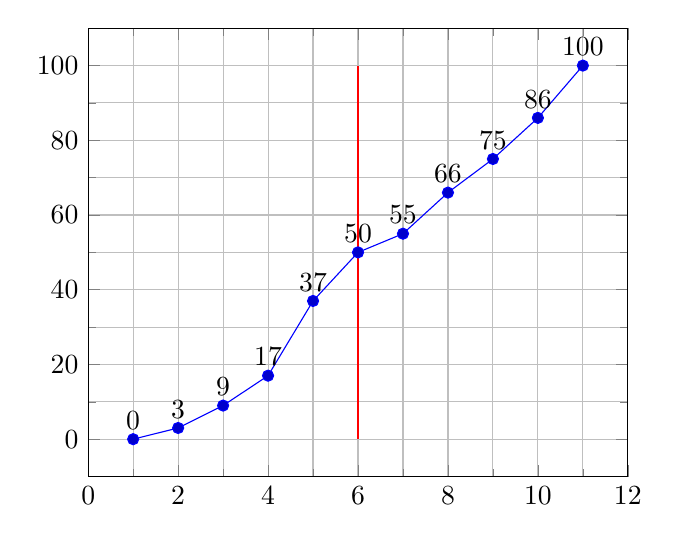
\begin{tikzpicture}
\begin{axis}[grid=both,minor tick num=1]
   \addplot coordinates
      {(1,0)(2,3)(3,9)(4,17)(5,37)(6,50)(7,55)(8,66)(9,75)(10,86)(11,100)};
   \node [above] at (axis cs: 1,0) {$0$};
   \node [above] at (axis cs: 2,3) {$3$};
   \node [above] at (axis cs: 3,9) {$9$};
   \node [above] at (axis cs: 4,17) {$17$};
   \node [above] at (axis cs: 5,37) {$37$};
   \node [above] at (axis cs: 6,50) {$50$};
   \node [above] at (axis cs: 7,55) {$55$};
   \node [above] at (axis cs: 8,66) {$66$};
   \node [above] at (axis cs: 9,75) {$75$};
   \node [above] at (axis cs: 10,86) {$86$};
   \node [above] at (axis cs: 11,100) {$100$};

   \addplot[red,sharp plot,update limits=false] coordinates
      {(6,0)(6,100)};
\end{axis}
\end{tikzpicture}
\end{adjustbox}
\end{center}
\caption[Gerechtigkeitseinschätzungen von Teilnehmer 38]{Gerechtigkeitseinschätzungen von Teilnehmer 38}
\end{figure}

\begin{figure}[H]
\begin{center}
\begin{adjustbox}{max width=0.25\textwidth}
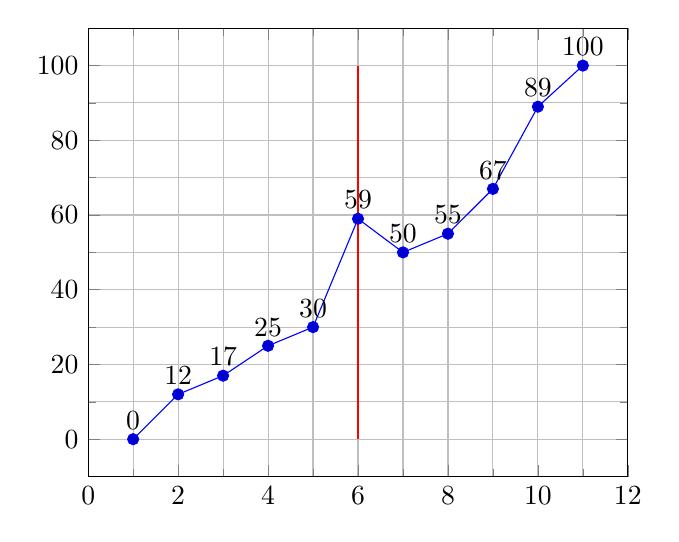
\begin{tikzpicture}
\begin{axis}[grid=both,minor tick num=1]
   \addplot coordinates
      {(1,0)(2,12)(3,17)(4,25)(5,30)(6,59)(7,50)(8,55)(9,67)(10,89)(11,100)};
   \node [above] at (axis cs: 1,0) {$0$};
   \node [above] at (axis cs: 2,12) {$12$};
   \node [above] at (axis cs: 3,17) {$17$};
   \node [above] at (axis cs: 4,25) {$25$};
   \node [above] at (axis cs: 5,30) {$30$};
   \node [above] at (axis cs: 6,59) {$59$};
   \node [above] at (axis cs: 7,50) {$50$};
   \node [above] at (axis cs: 8,55) {$55$};
   \node [above] at (axis cs: 9,67) {$67$};
   \node [above] at (axis cs: 10,89) {$89$};
   \node [above] at (axis cs: 11,100) {$100$};

   \addplot[red,sharp plot,update limits=false] coordinates
      {(6,0)(6,100)};
\end{axis}
\end{tikzpicture}
\end{adjustbox}
\end{center}
\caption[Gerechtigkeitseinschätzungen von Teilnehmer 39]{Gerechtigkeitseinschätzungen von Teilnehmer 39}
\end{figure}

\begin{figure}[H]
\begin{center}
\begin{adjustbox}{max width=0.25\textwidth}
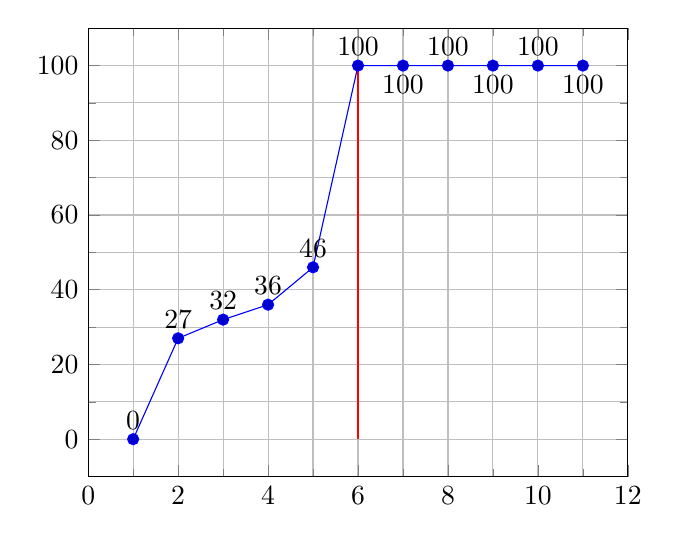
\begin{tikzpicture}
\begin{axis}[grid=both,minor tick num=1]
   \addplot coordinates
      {(1,0)(2,27)(3,32)(4,36)(5,46)(6,100)(7,100)(8,100)(9,100)(10,100)(11,100)};
   \node [above] at (axis cs: 1,0) {$0$};
   \node [above] at (axis cs: 2,27) {$27$};
   \node [above] at (axis cs: 3,32) {$32$};
   \node [above] at (axis cs: 4,36) {$36$};
   \node [above] at (axis cs: 5,46) {$46$};
   \node [above] at (axis cs: 6,100) {$100$};
   \node [below] at (axis cs: 7,100) {$100$};
   \node [above] at (axis cs: 8,100) {$100$};
   \node [below] at (axis cs: 9,100) {$100$};
   \node [above] at (axis cs: 10,100) {$100$};
   \node [below] at (axis cs: 11,100) {$100$};

   \addplot[red,sharp plot,update limits=false] coordinates
      {(6,0)(6,100)};
\end{axis}
\end{tikzpicture}
\end{adjustbox}
\end{center}
\caption[Gerechtigkeitseinschätzungen von Teilnehmer 40]{Gerechtigkeitseinschätzungen von Teilnehmer 40}
\end{figure}

\begin{figure}[H]
\begin{center}
\begin{adjustbox}{max width=0.25\textwidth}
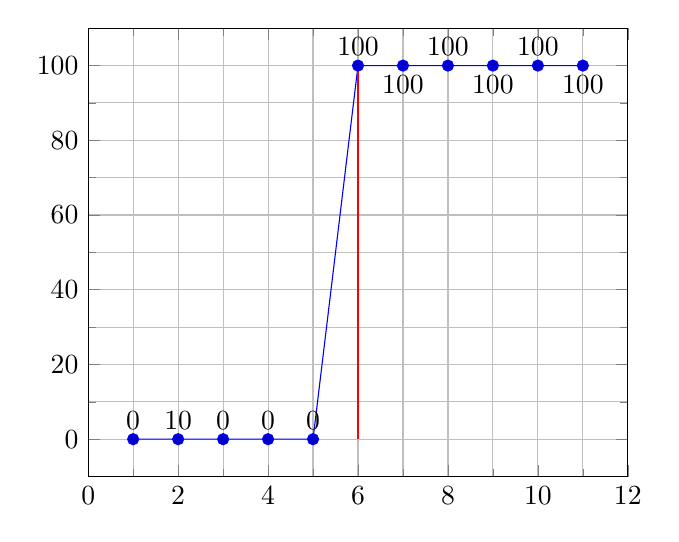
\begin{tikzpicture}
\begin{axis}[grid=both,minor tick num=1]
   \addplot coordinates
      {(1,0)(2,0)(3,0)(4,0)(5,0)(6,100)(7,100)(8,100)(9,100)(10,100)(11,100)};
   \node [above] at (axis cs: 1,0) {$0$};
   \node [above] at (axis cs: 2,0) {$10$};
   \node [above] at (axis cs: 3,0) {$0$};
   \node [above] at (axis cs: 4,0) {$0$};
   \node [above] at (axis cs: 5,0) {$0$};
   \node [above] at (axis cs: 6,100) {$100$};
   \node [below] at (axis cs: 7,100) {$100$};
   \node [above] at (axis cs: 8,100) {$100$};
   \node [below] at (axis cs: 9,100) {$100$};
   \node [above] at (axis cs: 10,100) {$100$};
   \node [below] at (axis cs: 11,100) {$100$};

   \addplot[red,sharp plot,update limits=false] coordinates
      {(6,0)(6,100)};
\end{axis}
\end{tikzpicture}
\end{adjustbox}
\end{center}
\caption[Gerechtigkeitseinschätzungen von Teilnehmer 41]{Gerechtigkeitseinschätzungen von Teilnehmer 41}
\end{figure}

\begin{figure}[H]
\begin{center}
\begin{adjustbox}{max width=0.25\textwidth}
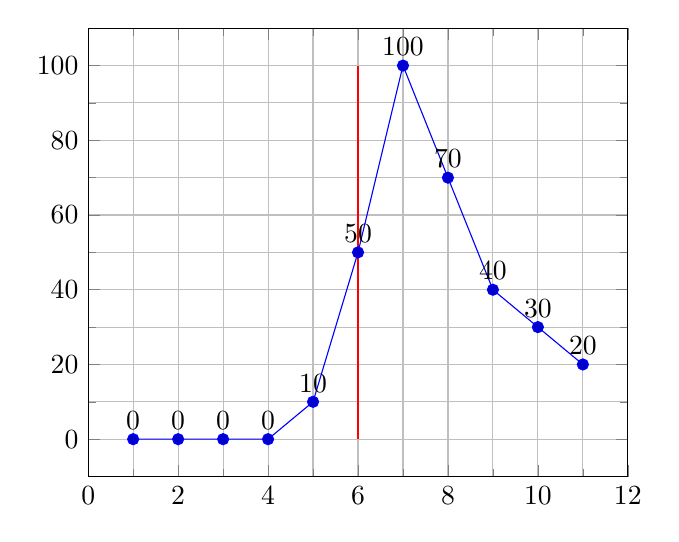
\begin{tikzpicture}
\begin{axis}[grid=both,minor tick num=1]
   \addplot coordinates
      {(1,0)(2,0)(3,0)(4,0)(5,10)(6,50)(7,100)(8,70)(9,40)(10,30)(11,20)};
   \node [above] at (axis cs: 1,0) {$0$};
   \node [above] at (axis cs: 2,0) {$0$};
   \node [above] at (axis cs: 3,0) {$0$};
   \node [above] at (axis cs: 4,0) {$0$};
   \node [above] at (axis cs: 5,10) {$10$};
   \node [above] at (axis cs: 6,50) {$50$};
   \node [above] at (axis cs: 7,100) {$100$};
   \node [above] at (axis cs: 8,70) {$70$};
   \node [above] at (axis cs: 9,40) {$40$};
   \node [above] at (axis cs: 10,30) {$30$};
   \node [above] at (axis cs: 11,20) {$20$};

   \addplot[red,sharp plot,update limits=false] coordinates
      {(6,0)(6,100)};
\end{axis}
\end{tikzpicture}
\end{adjustbox}
\end{center}
\caption[Gerechtigkeitseinschätzungen von Teilnehmer 42]{Gerechtigkeitseinschätzungen von Teilnehmer 42}
\end{figure}

\begin{figure}[H]
\begin{center}
\begin{adjustbox}{max width=0.25\textwidth}
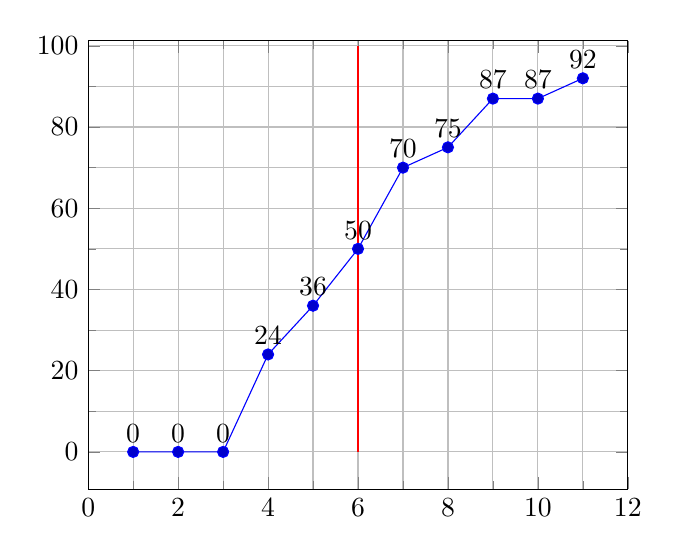
\begin{tikzpicture}
\begin{axis}[grid=both,minor tick num=1]
   \addplot coordinates
      {(1,0)(2,0)(3,0)(4,24)(5,36)(6,50)(7,70)(8,75)(9,87)(10,87)(11,92)};
   \node [above] at (axis cs: 1,0) {$0$};
   \node [above] at (axis cs: 2,0) {$0$};
   \node [above] at (axis cs: 3,0) {$0$};
   \node [above] at (axis cs: 4,24) {$24$};
   \node [above] at (axis cs: 5,36) {$36$};
   \node [above] at (axis cs: 6,50) {$50$};
   \node [above] at (axis cs: 7,70) {$70$};
   \node [above] at (axis cs: 8,75) {$75$};
   \node [above] at (axis cs: 9,87) {$87$};
   \node [above] at (axis cs: 10,87) {$87$};
   \node [above] at (axis cs: 11,92) {$92$};

   \addplot[red,sharp plot,update limits=false] coordinates
      {(6,0)(6,100)};
\end{axis}
\end{tikzpicture}
\end{adjustbox}
\end{center}
\caption[Gerechtigkeitseinschätzungen von Teilnehmer 43]{Gerechtigkeitseinschätzungen von Teilnehmer 43}
\end{figure}

\begin{figure}[H]
\begin{center}
\begin{adjustbox}{max width=0.25\textwidth}
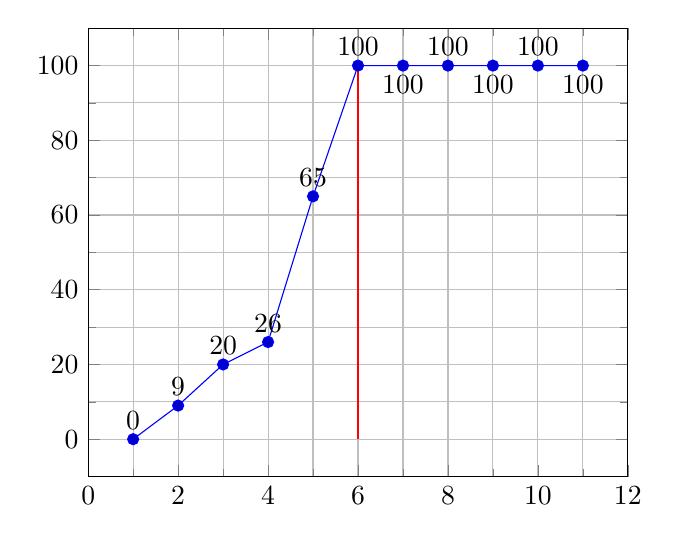
\begin{tikzpicture}
\begin{axis}[grid=both,minor tick num=1]
   \addplot coordinates
      {(1,0)(2,9)(3,20)(4,26)(5,65)(6,100)(7,100)(8,100)(9,100)(10,100)(11,100)};
   \node [above] at (axis cs: 1,0) {$0$};
   \node [above] at (axis cs: 2,9) {$9$};
   \node [above] at (axis cs: 3,20) {$20$};
   \node [above] at (axis cs: 4,26) {$26$};
   \node [above] at (axis cs: 5,65) {$65$};
   \node [above] at (axis cs: 6,100) {$100$};
   \node [below] at (axis cs: 7,100) {$100$};
   \node [above] at (axis cs: 8,100) {$100$};
   \node [below] at (axis cs: 9,100) {$100$};
   \node [above] at (axis cs: 10,100) {$100$};
   \node [below] at (axis cs: 11,100) {$100$};

   \addplot[red,sharp plot,update limits=false] coordinates
      {(6,0)(6,100)};
\end{axis}
\end{tikzpicture}
\end{adjustbox}
\end{center}
\caption[Gerechtigkeitseinschätzungen von Teilnehmer 44]{Gerechtigkeitseinschätzungen von Teilnehmer 44}
\end{figure}

\begin{figure}[H]
\begin{center}
\begin{adjustbox}{max width=0.25\textwidth}
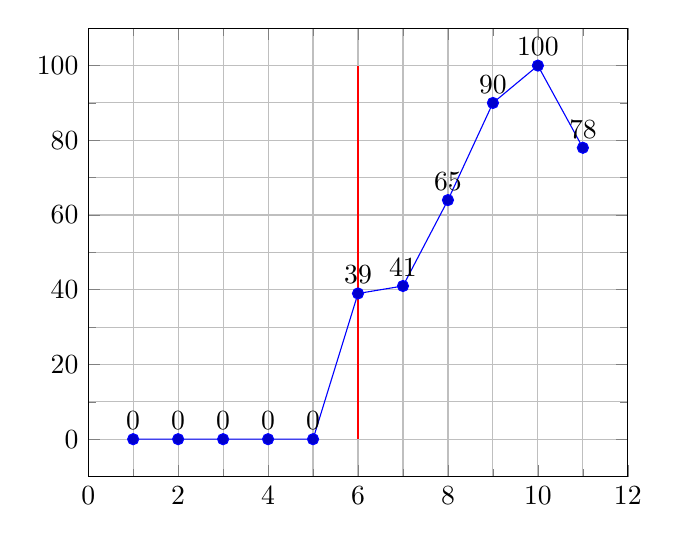
\begin{tikzpicture}
\begin{axis}[grid=both,minor tick num=1]
   \addplot coordinates
      {(1,0)(2,0)(3,0)(4,0)(5,0)(6,39)(7,41)(8,64)(9,90)(10,100)(11,78)};
   \node [above] at (axis cs: 1,0) {$0$};
   \node [above] at (axis cs: 2,0) {$0$};
   \node [above] at (axis cs: 3,0) {$0$};
   \node [above] at (axis cs: 4,0) {$0$};
   \node [above] at (axis cs: 5,0) {$0$};
   \node [above] at (axis cs: 6,39) {$39$};
   \node [above] at (axis cs: 7,41) {$41$};
   \node [above] at (axis cs: 8,64) {$65$};
   \node [above] at (axis cs: 9,90) {$90$};
   \node [above] at (axis cs: 10,100) {$100$};
   \node [above] at (axis cs: 11,78) {$78$};

   \addplot[red,sharp plot,update limits=false] coordinates
      {(6,0)(6,100)};
\end{axis}
\end{tikzpicture}
\end{adjustbox}
\end{center}
\caption[Gerechtigkeitseinschätzungen von Teilnehmer 45]{Gerechtigkeitseinschätzungen von Teilnehmer 45}
\end{figure}

\begin{figure}[H]
\begin{center}
\begin{adjustbox}{max width=0.25\textwidth}
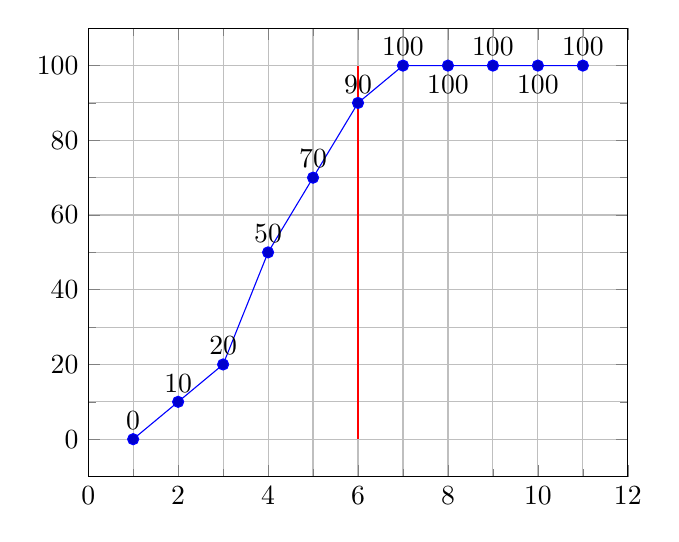
\begin{tikzpicture}
\begin{axis}[grid=both,minor tick num=1]
   \addplot coordinates
      {(1,0)(2,10)(3,20)(4,50)(5,70)(6,90)(7,100)(8,100)(9,100)(10,100)(11,100)};
   \node [above] at (axis cs: 1,0) {$0$};
   \node [above] at (axis cs: 2,10) {$10$};
   \node [above] at (axis cs: 3,20) {$20$};
   \node [above] at (axis cs: 4,50) {$50$};
   \node [above] at (axis cs: 5,70) {$70$};
   \node [above] at (axis cs: 6,90) {$90$};
   \node [above] at (axis cs: 7,100) {$100$};
   \node [below] at (axis cs: 8,100) {$100$};
   \node [above] at (axis cs: 9,100) {$100$};
   \node [below] at (axis cs: 10,100) {$100$};
   \node [above] at (axis cs: 11,100) {$100$};

   \addplot[red,sharp plot,update limits=false] coordinates
      {(6,0)(6,100)};
\end{axis}
\end{tikzpicture}
\end{adjustbox}
\end{center}
\caption[Gerechtigkeitseinschätzungen von Teilnehmer 46]{Gerechtigkeitseinschätzungen von Teilnehmer 46}
\end{figure}

\begin{figure}[H]
\begin{center}
\begin{adjustbox}{max width=0.25\textwidth}
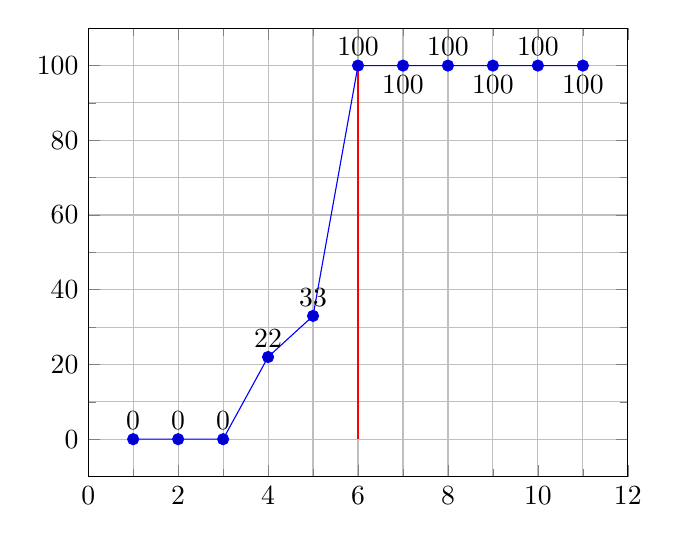
\begin{tikzpicture}
\begin{axis}[grid=both,minor tick num=1]
   \addplot coordinates
      {(1,0)(2,0)(3,0)(4,22)(5,33)(6,100)(7,100)(8,100)(9,100)(10,100)(11,100)};
   \node [above] at (axis cs: 1,0) {$0$};
   \node [above] at (axis cs: 2,0) {$0$};
   \node [above] at (axis cs: 3,0) {$0$};
   \node [above] at (axis cs: 4,22) {$22$};
   \node [above] at (axis cs: 5,33) {$33$};
   \node [above] at (axis cs: 6,100) {$100$};
   \node [below] at (axis cs: 7,100) {$100$};
   \node [above] at (axis cs: 8,100) {$100$};
   \node [below] at (axis cs: 9,100) {$100$};
   \node [above] at (axis cs: 10,100) {$100$};
   \node [below] at (axis cs: 11,100) {$100$};

   \addplot[red,sharp plot,update limits=false] coordinates
      {(6,0)(6,100)};
\end{axis}
\end{tikzpicture}
\end{adjustbox}
\end{center}
\caption[Gerechtigkeitseinschätzungen von Teilnehmer 47]{Gerechtigkeitseinschätzungen von Teilnehmer 47}
\end{figure}

\begin{figure}[H]
\begin{center}
\begin{adjustbox}{max width=0.25\textwidth}
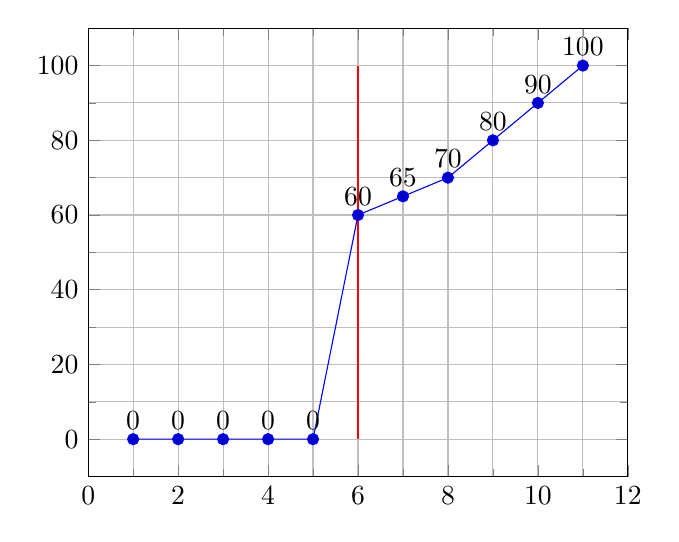
\begin{tikzpicture}
\begin{axis}[grid=both,minor tick num=1]
   \addplot coordinates
      {(1,0)(2,0)(3,0)(4,0)(5,0)(6,60)(7,65)(8,70)(9,80)(10,90)(11,100)};
   \node [above] at (axis cs: 1,0) {$0$};
   \node [above] at (axis cs: 2,0) {$0$};
   \node [above] at (axis cs: 3,0) {$0$};
   \node [above] at (axis cs: 4,0) {$0$};
   \node [above] at (axis cs: 5,0) {$0$};
   \node [above] at (axis cs: 6,60) {$60$};
   \node [above] at (axis cs: 7,65) {$65$};
   \node [above] at (axis cs: 8,70) {$70$};
   \node [above] at (axis cs: 9,80) {$80$};
   \node [above] at (axis cs: 10,90) {$90$};
   \node [above] at (axis cs: 11,100) {$100$};

   \addplot[red,sharp plot,update limits=false] coordinates
      {(6,0)(6,100)};
\end{axis}
\end{tikzpicture}
\end{adjustbox}
\end{center}
\caption[Gerechtigkeitseinschätzungen von Teilnehmer 48]{Gerechtigkeitseinschätzungen von Teilnehmer 48}
\end{figure}

\begin{figure}[H]
\begin{center}
\begin{adjustbox}{max width=0.25\textwidth}
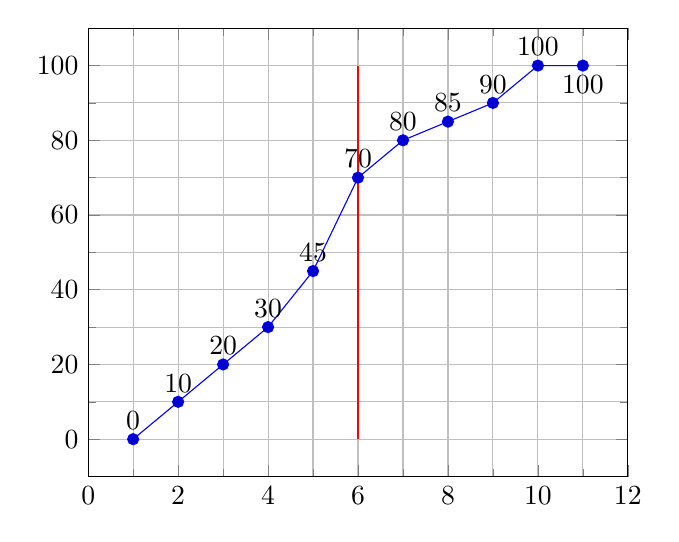
\begin{tikzpicture}
\begin{axis}[grid=both,minor tick num=1]
   \addplot coordinates
      {(1,0)(2,10)(3,20)(4,30)(5,45)(6,70)(7,80)(8,85)(9,90)(10,100)(11,100)};
   \node [above] at (axis cs: 1,0) {$0$};
   \node [above] at (axis cs: 2,10) {$10$};
   \node [above] at (axis cs: 3,20) {$20$};
   \node [above] at (axis cs: 4,30) {$30$};
   \node [above] at (axis cs: 5,45) {$45$};
   \node [above] at (axis cs: 6,70) {$70$};
   \node [above] at (axis cs: 7,80) {$80$};
   \node [above] at (axis cs: 8,85) {$85$};
   \node [above] at (axis cs: 9,90) {$90$};
   \node [above] at (axis cs: 10,100) {$100$};
   \node [below] at (axis cs: 11,100) {$100$};

   \addplot[red,sharp plot,update limits=false] coordinates
      {(6,0)(6,100)};
\end{axis}
\end{tikzpicture}
\end{adjustbox}
\end{center}
\caption[Gerechtigkeitseinschätzungen von Teilnehmer 49]{Gerechtigkeitseinschätzungen von Teilnehmer 49}
\end{figure}

\begin{figure}[H]
\begin{center}
\begin{adjustbox}{max width=0.25\textwidth}
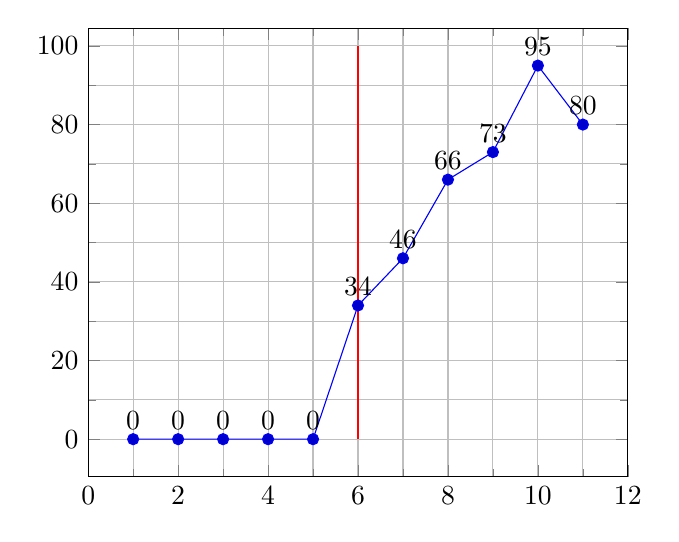
\begin{tikzpicture}
\begin{axis}[grid=both,minor tick num=1]
   \addplot coordinates
      {(1,0)(2,0)(3,0)(4,0)(5,0)(6,34)(7,46)(8,66)(9,73)(10,95)(11,80)};
   \node [above] at (axis cs: 1,0) {$0$};
   \node [above] at (axis cs: 2,0) {$0$};
   \node [above] at (axis cs: 3,0) {$0$};
   \node [above] at (axis cs: 4,0) {$0$};
   \node [above] at (axis cs: 5,0) {$0$};
   \node [above] at (axis cs: 6,34) {$34$};
   \node [above] at (axis cs: 7,46) {$46$};
   \node [above] at (axis cs: 8,66) {$66$};
   \node [above] at (axis cs: 9,73) {$73$};
   \node [above] at (axis cs: 10,95) {$95$};
   \node [above] at (axis cs: 11,80) {$80$};

   \addplot[red,sharp plot,update limits=false] coordinates
      {(6,0)(6,100)};
\end{axis}
\end{tikzpicture}
\end{adjustbox}
\end{center}
\caption[Gerechtigkeitseinschätzungen von Teilnehmer 50]{Gerechtigkeitseinschätzungen von Teilnehmer 50}
\end{figure}

\begin{figure}[H]
\begin{center}
\begin{adjustbox}{max width=0.25\textwidth}
\begin{tikzpicture}
\begin{axis}[grid=both,minor tick num=1]
   \addplot coordinates
      {(1,0)(2,9)(3,20)(4,38)(5,50)(6,100)(7,100)(8,100)(9,100)(10,100)(11,100)};
   \node [above] at (axis cs: 1,0) {$0$};
   \node [above] at (axis cs: 2,9) {$9$};
   \node [above] at (axis cs: 3,20) {$20$};
   \node [above] at (axis cs: 4,38) {$38$};
   \node [above] at (axis cs: 5,50) {$50$};
   \node [above] at (axis cs: 6,100) {$100$};
   \node [below] at (axis cs: 7,100) {$100$};
   \node [above] at (axis cs: 8,100) {$100$};
   \node [below] at (axis cs: 9,100) {$100$};
   \node [above] at (axis cs: 10,100) {$100$};
   \node [below] at (axis cs: 11,100) {$100$};

   \addplot[red,sharp plot,update limits=false] coordinates
      {(6,0)(6,100)};
\end{axis}
\end{tikzpicture}
\end{adjustbox}
\end{center}
\caption[Gerechtigkeitseinschätzungen von Teilnehmer 51]{Gerechtigkeitseinschätzungen von Teilnehmer 51}
\end{figure}

\begin{figure}[H]
\begin{center}
\begin{adjustbox}{max width=0.25\textwidth}
\begin{tikzpicture}
\begin{axis}[grid=both,minor tick num=1]
   \addplot coordinates
      {(1,0)(2,0)(3,0)(4,0)(5,25)(6,70)(7,80)(8,90)(9,100)(10,90)(11,85)};
   \node [above] at (axis cs: 1,0) {$0$};
   \node [above] at (axis cs: 2,0) {$0$};
   \node [above] at (axis cs: 3,0) {$0$};
   \node [above] at (axis cs: 4,0) {$0$};
   \node [above] at (axis cs: 5,25) {$25$};
   \node [above] at (axis cs: 6,70) {$70$};
   \node [above] at (axis cs: 7,80) {$80$};
   \node [above] at (axis cs: 8,90) {$90$};
   \node [above] at (axis cs: 9,100) {$100$};
   \node [above] at (axis cs: 10,90) {$90$};
   \node [above] at (axis cs: 11,85) {$85$};

   \addplot[red,sharp plot,update limits=false] coordinates
      {(6,0)(6,100)};
\end{axis}
\end{tikzpicture}
\end{adjustbox}
\end{center}
\caption[Gerechtigkeitseinschätzungen von Teilnehmer 52]{Gerechtigkeitseinschätzungen von Teilnehmer 52}
\end{figure}

\begin{figure}[H]
\centering
\includegraphics[width=0.5\textwidth]{figures/verteil_0.png}
\caption[Häufigkeit der Gerechtigkeitseinschätzungen für Verteilung 0]{Häufigkeit der Gerechtigkeitseinschätzungen für Verteilung 0}
\end{figure}

\begin{figure}[H]
\centering
\includegraphics[width=0.5\textwidth]{figures/verteil_20.png}
\caption[Häufigkeit der Gerechtigkeitseinschätzungen für Verteilung 20]{Häufigkeit der Gerechtigkeitseinschätzungen für Verteilung 20}
\end{figure}

\begin{figure}[H]
\centering
\includegraphics[width=0.5\textwidth]{figures/verteil_40.png}
\caption[Häufigkeit der Gerechtigkeitseinschätzungen für Verteilung 40]{Häufigkeit der Gerechtigkeitseinschätzungen für Verteilung 40}
\end{figure}

\begin{figure}[H]
\centering
\includegraphics[width=0.5\textwidth]{figures/verteil_60.png}
\caption[Häufigkeit der Gerechtigkeitseinschätzungen für Verteilung 60]{Häufigkeit der Gerechtigkeitseinschätzungen für Verteilung 60}
\end{figure}

\begin{figure}[H]
\centering
\includegraphics[width=0.5\textwidth]{figures/verteil_80.png}
\caption[Häufigkeit der Gerechtigkeitseinschätzungen für Verteilung 80]{Häufigkeit der Gerechtigkeitseinschätzungen für Verteilung 80}
\end{figure}

\begin{figure}[H]
\centering
\includegraphics[width=0.5\textwidth]{figures/verteil_100.png}
\caption[Häufigkeit der Gerechtigkeitseinschätzungen für Verteilung 100]{Häufigkeit der Gerechtigkeitseinschätzungen für Verteilung 100}
\end{figure}

\begin{figure}[H]
\centering
\includegraphics[width=0.5\textwidth]{figures/verteil_120.png}
\caption[Häufigkeit der Gerechtigkeitseinschätzungen für Verteilung 120]{Häufigkeit der Gerechtigkeitseinschätzungen für Verteilung 120}
\end{figure}

\begin{figure}[H]
\centering
\includegraphics[width=0.5\textwidth]{figures/verteil_140.png}
\caption[Häufigkeit der Gerechtigkeitseinschätzungen für Verteilung 140]{Häufigkeit der Gerechtigkeitseinschätzungen für Verteilung 140}
\end{figure}

\begin{figure}[H]
\centering
\includegraphics[width=0.5\textwidth]{figures/verteil_160.png}
\caption[Häufigkeit der Gerechtigkeitseinschätzungen für Verteilung 160]{Häufigkeit der Gerechtigkeitseinschätzungen für Verteilung 160}
\end{figure}

\begin{figure}[H]
\centering
\includegraphics[width=0.5\textwidth]{figures/verteil_180.png}
\caption[Häufigkeit der Gerechtigkeitseinschätzungen für Verteilung 180]{Häufigkeit der Gerechtigkeitseinschätzungen für Verteilung 180}
\end{figure}

\begin{figure}[H]
\centering
\includegraphics[width=0.5\textwidth]{figures/verteil_200.png}
\caption[Häufigkeit der Gerechtigkeitseinschätzungen für Verteilung 200]{Häufigkeit der Gerechtigkeitseinschätzungen für Verteilung 200}
\end{figure}

\begin{figure}[H]
\centering
\includegraphics[width=0.5\textwidth]{figures/streu_2d.png}
\caption[Zweidimensionales Streudiagramm]{Zweidimensionales Streudiagramm}
\end{figure}

\begin{figure}[H]
\centering
\includegraphics[width=0.5\textwidth]{figures/streu_2d_mittel.png}
\caption[Zweidimensionales Streudiagramm mit Mittelwerten]{Zweidimensionales Streudiagramm mit Mittelwerten}
\end{figure}

\begin{figure}[H]
\centering
\includegraphics[width=0.5\textwidth]{figures/konfi.png}
\caption[95-Prozent-Konfidenzintervalle]{95-Prozent-Konfidenzintervalle}
\end{figure}

\begin{figure}[H]
\begin{center}
\begin{tikzpicture}
\begin{axis}[xlabel=Bedarfslücke,ylabel=Gerechtigkeit]
   \addplot coordinates
      {(-10,10) (0,0) (10,10)};
\end{axis}
\end{tikzpicture}
\end{center}
\caption[Zweidimensionale Darstellung wechselnder Monotonie]{Zweidimensionale Darstellung wechselnder Monotonie}
\end{figure}

\begin{figure}[H]
\begin{center}
\begin{tikzpicture}
\begin{axis}[xlabel=$x$,ylabel=$y$,zlabel=$z$,y dir=reverse,colormap/GnBu,axis lines=box]
\addplot3[surf] coordinates
{
(0,0,0) (1,0,1) (2,0,2) (3,0,3) (4,0,4) (5,0,5) (6,0,6) (7,0,7) (8,0,8) (9,0,9) (10,0,10)

(0,1,1) (1,1,0) (2,1,1) (3,1,2) (4,1,3) (5,1,4) (6,1,5) (7,1,6) (8,1,7) (9,1,8) (10,1,9)

(0,2,2) (1,2,1) (2,2,0) (3,2,1) (4,2,2) (5,2,3) (6,2,4) (7,2,5) (8,2,6) (9,2,7) (10,2,8)

(0,3,3) (1,3,2) (2,3,1) (3,3,0) (4,3,1) (5,3,2) (6,3,3) (7,3,4) (8,3,5) (9,3,6) (10,3,7)

(0,4,4) (1,4,3) (2,4,2) (3,4,1) (4,4,0) (5,4,1) (6,4,2) (7,4,3) (8,4,4) (9,4,5) (10,4,6)

(0,5,5) (1,5,4) (2,5,3) (3,5,2) (4,5,1) (5,5,0) (6,5,1) (7,5,2) (8,5,3) (9,5,4) (10,5,5)

(0,6,6) (1,6,5) (2,6,4) (3,6,3) (4,6,2) (5,6,1) (6,6,0) (7,6,1) (8,6,2) (9,6,3) (10,6,4)

(0,7,7) (1,7,6) (2,7,5) (3,7,4) (4,7,3) (5,7,2) (6,7,1) (7,7,0) (8,7,1) (9,7,2) (10,7,3)

(0,8,8) (1,8,7) (2,8,6) (3,8,5) (4,8,4) (5,8,3) (6,8,2) (7,8,1) (8,8,0) (9,8,1) (10,8,2)

(0,9,9) (1,9,8) (2,9,7) (3,9,6) (4,9,5) (5,9,4) (6,9,3) (7,9,2) (8,9,1) (9,9,0) (10,9,1)

(0,10,10) (1,10,9) (2,10,8) (3,10,7) (4,10,6) (5,10,5) (6,10,4) (7,10,3) (8,10,2) (9,10,1) 
(10,10,0)
};
\end{axis}
\end{tikzpicture}
\end{center}
\caption[Dreidimensionale Darstellung wechselnder Monotonie]{Dreidimensionale Darstellung wechselnder Monotonie}
\end{figure}

\begin{figure}[H]
\begin{center}
\begin{tikzpicture}
\begin{axis}[xlabel=Bedarfslücke,ylabel=Gerechtigkeit]
   \addplot coordinates
      {(-10,10) (0,0) (10,-10)};
\end{axis}
\end{tikzpicture}
\end{center}
\caption[Zweidimensionale Darstellung kontinuierlich steigender Monotonie]{Zweidimensionale Darstellung kontinuierlich steigender Monotonie}
\end{figure}

\begin{figure}[H]
\begin{center}
\begin{tikzpicture}
\begin{axis}[xlabel=$x$,ylabel =$y$,zlabel =$z$,y dir=reverse,colormap/GnBu,axis lines=box]
\addplot3[surf] coordinates
{
(0,0,0) (1,0,1) (2,0,2) (3,0,3) (4,0,4) (5,0,5) (6,0,6) (7,0,7) (8,0,8) (9,0,9) (10,0,10)

(0,1,-1) (1,1,0) (2,1,1) (3,1,2) (4,1,3) (5,1,4) (6,1,5) (7,1,6) (8,1,7) (9,1,8) (10,1,9)

(0,2,-2) (1,2,-1) (2,2,0) (3,2,1) (4,2,2) (5,2,3) (6,2,4) (7,2,5) (8,2,6) (9,2,7) (10,2,8)

(0,3,-3) (1,3,-2) (2,3,-1) (3,3,0) (4,3,1) (5,3,2) (6,3,3) (7,3,4) (8,3,5) (9,3,6) (10,3,7)

(0,4,-4) (1,4,-3) (2,4,-2) (3,4,-1) (4,4,0) (5,4,1) (6,4,2) (7,4,3) (8,4,4) (9,4,5) (10,4,6)

(0,5,-5) (1,5,-4) (2,5,-3) (3,5,-2) (4,5,-1) (5,5,0) (6,5,1) (7,5,2) (8,5,3) (9,5,4) (10,5,5)

(0,6,-6) (1,6,-5) (2,6,-4) (3,6,-3) (4,6,-2) (5,6,-1) (6,6,0) (7,6,1) (8,6,2) (9,6,3) (10,6,4)

(0,7,-7) (1,7,-6) (2,7,-5) (3,7,-4) (4,7,-3) (5,7,-2) (6,7,-1) (7,7,0) (8,7,1) (9,7,2) (10,7,3)

(0,8,-8) (1,8,-7) (2,8,-6) (3,8,-5) (4,8,-4) (5,8,-3) (6,8,-2) (7,8,-1) (8,8,0) (9,8,1) (10,8,2)

(0,9,-9) (1,9,-8) (2,9,-7) (3,9,-6) (4,9,-5) (5,9,-4) (6,9,-3) (7,9,-2) (8,9,-1) (9,9,0) (10,9,1)

(0,10,-10) (1,10,-9) (2,10,-8) (3,10,-7) (4,10,-6) (5,10,-5) (6,10,-4) (7,10,-3) (8,10,-2) (9,10,-1) (10,10,0)
};
\end{axis}
\end{tikzpicture}
\end{center}
\caption[Dreidimensionale Darstellung kontinuierlich steigender Monotonie]{Dreidimensionale Darstellung kontinuierlich steigender Monotonie}
\end{figure}

\begin{figure}[H]
\begin{center}
\begin{tikzpicture}
\begin{axis}[ylabel=Gerechtigkeit,xlabel=Bedarfslücke]
   \addplot+[smooth] coordinates
      {(-10,10) (-7.5,2.5) (0,0)};
   \addplot+[smooth] coordinates
      {(10,-10) (7.5,-2.5) (0,0)};
   \addplot+[smooth] coordinates
      {(0,0) (7.5,2.5) (10,10)};
\end{axis}
\end{tikzpicture}
\end{center}
\caption[Zweidimensionale Darstellung konkaver Monotoniesensitivitäten]{Zweidimensionale Darstellung konkaver Monotoniesensitivitäten}
\end{figure}

\begin{figure}[H]
\begin{center}
\begin{tikzpicture}
\begin{axis}[xlabel =$x$, ylabel =$y$,y dir=reverse,colormap/GnBu]
\addplot3[surf] coordinates
{
(0,0,0) (1,0,1^2) (2,0,2^2) (3,0,3^2) (4,0,4^2) (5,0,5^2) (6,0,6^2) (7,0,7^2) (8,0,8^2) (9,0,9^2) (10,0,10^2)

(0,1,-1^2) (1,1,0) (2,1,1^2) (3,1,2^2) (4,1,3^2) (5,1,4^2) (6,1,5^2) (7,1,6^2) (8,1,7^2) (9,1,8^2) (10,1,9^2)

(0,2,-2^2) (1,2,-1^2) (2,2,0) (3,2,1^2) (4,2,2^2) (5,2,3^2) (6,2,4^2) (7,2,5^2) (8,2,6^2) (9,2,7^2) (10,2,8^2)

(0,3,-3^2) (1,3,-2^2) (2,3,-1^2) (3,3,0) (4,3,1^2) (5,3,2^2) (6,3,3^2) (7,3,4^2) (8,3,5^2) (9,3,6^2) (10,3,7^2)

(0,4,-4^2) (1,4,-3^2) (2,4,-2^2) (3,4,-1^2) (4,4,0) (5,4,1^2) (6,4,2^2) (7,4,3^2) (8,4,4^2) (9,4,5^2) (10,4,6^2)

(0,5,-5^2) (1,5,-4^2) (2,5,-3^2) (3,5,-2^2) (4,5,-1^2) (5,5,0) (6,5,1^2) (7,5,2^2) (8,5,3^2) (9,5,4^2) (10,5,5^2)

(0,6,-6^2) (1,6,-5^2) (2,6,-4^2) (3,6,-3^2) (4,6,-2^2) (5,6,-1^2) (6,6,0) (7,6,1^2) (8,6,2^2) (9,6,3^2) (10,6,4^2)

(0,7,-7^2) (1,7,-6^2) (2,7,-5^2) (3,7,-4^2) (4,7,-3^2) (5,7,-2^2) (6,7,-1^2) (7,7,0) (8,7,1^2) (9,7,2^2) (10,7,3^2)

(0,8,-8^2) (1,8,-7^2) (2,8,-6^2) (3,8,-5^2) (4,8,-4^2) (5,8,-3^2) (6,8,-2^2) (7,8,-1^2) (8,8,0) (9,8,1^2) (10,8,2^2)

(0,9,-9^2) (1,9,-8^2) (2,9,-7^2) (3,9,-6^2) (4,9,-5^2) (5,9,-4^2) (6,9,-3^2) (7,9,-2^2) (8,9,-1^2) (9,9,0) (10,9,1^2)

(0,10,-10^2) (1,10,-9^2) (2,10,-8^2) (3,10,-7^2) (4,10,-6^2) (5,10,-5^2) (6,10,-4^2) (7,10,-3^2) (8,10,-2^2) (9,10,-1^2) (10,10,0)
};
\addplot3[surf] coordinates
{
(0,0,0) (1,0,1^2) (2,0,2^2) (3,0,3^2) (4,0,4^2) (5,0,5^2) (6,0,6^2) (7,0,7^2) (8,0,8^2) (9,0,9^2) (10,0,10^2)

(0,1,1^2) (1,1,0) (2,1,1^2) (3,1,2^2) (4,1,3^2) (5,1,4^2) (6,1,5^2) (7,1,6^2) (8,1,7^2) (9,1,8^2) (10,1,9^2)

(0,2,2^2) (1,2,1^2) (2,2,0) (3,2,1^2) (4,2,2^2) (5,2,3^2) (6,2,4^2) (7,2,5^2) (8,2,6^2) (9,2,7^2) (10,2,8^2)

(0,3,3^2) (1,3,2^2) (2,3,1^2) (3,3,0) (4,3,1^2) (5,3,2^2) (6,3,3^2) (7,3,4^2) (8,3,5^2) (9,3,6^2) (10,3,7^2)

(0,4,4^2) (1,4,3^2) (2,4,2^2) (3,4,1^2) (4,4,0) (5,4,1^2) (6,4,2^2) (7,4,3^2) (8,4,4^2) (9,4,5^2) (10,4,6^2)

(0,5,5^2) (1,5,4^2) (2,5,3^2) (3,5,2^2) (4,5,1^2) (5,5,0) (6,5,1^2) (7,5,2^2) (8,5,3^2) (9,5,4^2) (10,5,5^2)

(0,6,6^2) (1,6,5^2) (2,6,4^2) (3,6,3^2) (4,6,2^2) (5,6,1^2) (6,6,0) (7,6,1^2) (8,6,2^2) (9,6,3^2) (10,6,4^2)

(0,7,7^2) (1,7,6^2) (2,7,5^2) (3,7,4^2) (4,7,3^2) (5,7,2^2) (6,7,1^2) (7,7,0) (8,7,1^2) (9,7,2^2) (10,7,3^2)

(0,8,8^2) (1,8,7^2) (2,8,6^2) (3,8,5^2) (4,8,4^2) (5,8,3^2) (6,8,2^2) (7,8,1^2) (8,8,0) (9,8,1^2) (10,8,2^2)

(0,9,9^2) (1,9,8^2) (2,9,7^2) (3,9,6^2) (4,9,5^2) (5,9,4^2) (6,9,3^2) (7,9,2^2) (8,9,1^2) (9,9,0) (10,9,1^2)

(0,10,10^2) (1,10,9^2) (2,10,8^2) (3,10,7^2) (4,10,6^2) (5,10,5^2) (6,10,4^2) (7,10,3^2) (8,10,2^2) (9,10,1^2)  (10,10,0)
};
\end{axis}
\end{tikzpicture}
\end{center}
\caption[Dreidimensionale Darstellung konkaver Monotoniesensitivitäten]{Dreidimensionale Darstellung konkaver Monotoniesensitivitäten}
\end{figure}

\begin{figure}[H]
\begin{center}
\begin{tikzpicture}
\begin{axis}[ylabel=Gerechtigkeit,xlabel=Bedarfslücke]
   \addplot+[smooth] coordinates
      {(-10,10) (-2.5,8.5) (0,0)};
   \addplot+[smooth] coordinates
      {(10,-10) (2.5,-8.5) (0,0)};
   \addplot+[smooth] coordinates
      {(0,0) (2.5,8.5) (10,10)};
\end{axis}
\end{tikzpicture}
\end{center}
\caption[Zweidimensionale Darstellung konvexer Monotoniesensitivitäten]{Zweidimensionale Darstellung konvexer Monotoniesensitivitäten}
\end{figure}

\begin{figure}[H]
\begin{center}
\begin{tikzpicture}
\begin{axis}[xlabel =$x$,ylabel =$y$,zlabel =$z$,y dir=reverse,colormap/GnBu]
\addplot3[surf] coordinates
{
(0,0,0) (1,0,20-1^2) (2,0,40-2^2) (3,0,60-3^2) (4,0,80-4^2) (5,0,100-5^2) (6,0,120-6^2) (7,0,140-7^2) (8,0,160-8^2) (9,0,180-9^2) (10,0,200-10^2)

(0,1,-20+1^2) (1,1,0) (2,1,20-1^2) (3,1,40-2^2) (4,1,60-3^2) (5,1,80-4^2) (6,1,100-5^2) (7,1,120-6^2) (8,1,140-7^2) (9,1,160-8^2) (10,1,180-9^2)

(0,2,-40+2^2) (1,2,-20+1^2) (2,2,0) (3,2,20-1^2) (4,2,40-2^2) (5,2,60-3^2) (6,2,80-4^2) (7,2,100-5^2) (8,2,120-6^2) (9,2,140-7^2) (10,2,160-8^2)

(0,3,-60+3^2) (1,3,-40+2^2) (2,3,-20+1^2) (3,3,0) (4,3,20-1^2) (5,3,40-2^2) (6,3,60-3^2) (7,3,80-4^2) (8,3,100-5^2) (9,3,120-6^2) (10,3,140-7^2)

(0,4,-80+4^2) (1,4,-60+3^2) (2,4,-40+2^2) (3,4,-20+1^2) (4,4,0) (5,4,20-1^2) (6,4,40-2^2) (7,4,60-3^2) (8,4,80-4^2) (9,4,100-5^2) (10,4,120-6^2)

(0,5,-100+5^2) (1,5,-80+4^2) (2,5,-60+3^2) (3,5,-40+2^2) (4,5,-20+1^2) (5,5,0) (6,5,20-1^2) (7,5,40-2^2) (8,5,60-3^2) (9,5,80-4^2) (10,5,100-5^2)

(0,6,-120+6^2) (1,6,-100+5^2) (2,6,-80+4^2) (3,6,-60+3^2) (4,6,-40+2^2) (5,6,-20+1^2) (6,6,0) (7,6,20-1^2) (8,6,40-2^2) (9,6,60-3^2) (10,6,80-4^2)

(0,7,-140+7^2) (1,7,-120+6^2) (2,7,-100+5^2) (3,7,-80+4^2) (4,7,-60+3^2) (5,7,-40+2^2) (6,7,-20+1^2) (7,7,0) (8,7,20-1^2) (9,7,40-2^2) (10,7,60-3^2)

(0,8,-160+8^2) (1,8,-140+7^2) (2,8,-120+6^2) (3,8,-100+5^2) (4,8,-80+4^2) (5,8,-60+3^2) (6,8,-40+2^2) (7,8,-20+1^2) (8,8,0) (9,8,20-1^2) (10,8,40-2^2)

(0,9,-180+9^2) (1,9,-160+8^2) (2,9,-140+7^2) (3,9,-120+6^2) (4,9,-100+5^2) (5,9,-80+4^2) (6,9,-60+3^2) (7,9,-40+2^2) (8,9,-20+1^2) (9,9,0) (10,9,20-1^2)

(0,10,-200+10^2) (1,10,-180+9^2) (2,10,-160+8^2) (3,10,-140+7^2) (4,10,-120+6^2) (5,10,-100+5^2) (6,10,-80+4^2) (7,10,-60+3^2) (8,10,-40+2^2) (9,10,-20+1^2) 
(10,10,0)
};
\addplot3[surf] coordinates
{
(0,0,0) (1,0,20-1^2) (2,0,40-2^2) (3,0,60-3^2) (4,0,80-4^2) (5,0,100-5^2) (6,0,120-6^2) (7,0,140-7^2) (8,0,160-8^2) (9,0,180-9^2) (10,0,200-10^2)

(0,1,20-1^2) (1,1,0) (2,1,20-1^2) (3,1,40-2^2) (4,1,60-3^2) (5,1,80-4^2) (6,1,100-5^2) (7,1,120-6^2) (8,1,140-7^2) (9,1,160-8^2) (10,1,180-9^2)

(0,2,40-2^2) (1,2,20-1^2) (2,2,0) (3,2,20-1^2) (4,2,40-2^2) (5,2,60-3^2) (6,2,80-4^2) (7,2,100-5^2) (8,2,120-6^2) (9,2,140-7^2) (10,2,160-8^2)

(0,3,60-3^2) (1,3,40-2^2) (2,3,20-1^2) (3,3,0) (4,3,20-1^2) (5,3,40-2^2) (6,3,60-3^2) (7,3,80-4^2) (8,3,100-5^2) (9,3,120-6^2) (10,3,140-7^2)

(0,4,80-4^2) (1,4,60-3^2) (2,4,40-2^2) (3,4,20-1^2) (4,4,0) (5,4,20-1^2) (6,4,40-2^2) (7,4,60-3^2) (8,4,80-4^2) (9,4,100-5^2) (10,4,120-6^2)

(0,5,100-5^2) (1,5,80-4^2) (2,5,60-3^2) (3,5,40-2^2) (4,5,20-1^2) (5,5,0) (6,5,20-1^2) (7,5,40-2^2) (8,5,60-3^2) (9,5,80-4^2) (10,5,100-5^2)

(0,6,120-6^2) (1,6,100-5^2) (2,6,80-4^2) (3,6,60-3^2) (4,6,40-2^2) (5,6,20-1^2) (6,6,0) (7,6,20-1^2) (8,6,40-2^2) (9,6,60-3^2) (10,6,80-4^2)

(0,7,140-7^2) (1,7,120-6^2) (2,7,100-5^2) (3,7,80-4^2) (4,7,60-3^2) (5,7,40-2^2) (6,7,20-1^2) (7,7,0) (8,7,20-1^2) (9,7,40-2^2) (10,7,60-3^2)

(0,8,160-8^2) (1,8,140-7^2) (2,8,120-6^2) (3,8,100-5^2) (4,8,80-4^2) (5,8,60-3^2) (6,8,40-2^2) (7,8,20-1^2) (8,8,0) (9,8,20-1^2) (10,8,40-2^2)

(0,9,180-9^2) (1,9,160-8^2) (2,9,140-7^2) (3,9,120-6^2) (4,9,100-5^2) (5,9,80-4^2) (6,9,60-3^2) (7,9,40-2^2) (8,9,20-1^2) (9,9,0) (10,9,20-1^2)

(0,10,200-10^2) (1,10,180-9^2) (2,10,160-8^2) (3,10,140-7^2) (4,10,120-6^2) (5,10,100-5^2) (6,10,80-4^2) (7,10,60-3^2) (8,10,40-2^2) (9,10,20-1^2) 
(10,10,0)
};
\end{axis}
\end{tikzpicture}
\end{center}
\caption[Dreidimensionale Darstellung konvexer Monotoniesensitivitäten]{Dreidimensionale Darstellung konvexer Monotoniesensitivitäten}
\end{figure}

\begin{figure}[ht]
\begin{center}
\begin{tikzpicture}
\begin{axis}[xlabel=$x$,ylabel=$y$,zlabel=$z$,y dir=reverse,colormap/GnBu]
\addplot3[surf] coordinates
{
(0,0,0) (1,0,1^2) (2,0,2^2) (3,0,3^2) (4,0,4^2) (5,0,5^2) (6,0,6^2) (7,0,7^2) (8,0,8^2) (9,0,9^2) (10,0,10^2)

(0,1,-20+1^2) (1,1,0) (2,1,1^2) (3,1,2^2) (4,1,3^2) (5,1,4^2) (6,1,5^2) (7,1,6^2) (8,1,7^2) (9,1,8^2) (10,1,9^2)

(0,2,-40+2^2) (1,2,-20+1^2) (2,2,0) (3,2,1^2) (4,2,2^2) (5,2,3^2) (6,2,4^2) (7,2,5^2) (8,2,6^2) (9,2,7^2) (10,2,8^2)

(0,3,-60+3^2) (1,3,-40+2^2) (2,3,-20+1^2) (3,3,0) (4,3,1^2) (5,3,2^2) (6,3,3^2) (7,3,4^2) (8,3,5^2) (9,3,6^2) (10,3,7^2)

(0,4,-80+4^2) (1,4,-60+3^2) (2,4,-40+2^2) (3,4,-20+1^2) (4,4,0) (5,4,1^2) (6,4,2^2) (7,4,3^2) (8,4,4^2) (9,4,5^2) (10,4,6^2)

(0,5,-100+5^2) (1,5,-80+4^2) (2,5,-60+3^2) (3,5,-40+2^2) (4,5,-20+1^2) (5,5,0) (6,5,1^2) (7,5,2^2) (8,5,3^2) (9,5,4^2) (10,5,5^2)

(0,6,-120+6^2) (1,6,-100+5^2) (2,6,-80+4^2) (3,6,-60+3^2) (4,6,-40+2^2) (5,6,-20+1^2) (6,6,0) (7,6,1^2) (8,6,2^2) (9,6,3^2) (10,6,4^2)

(0,7,-140+7^2) (1,7,-120+6^2) (2,7,-100+5^2) (3,7,-80+4^2) (4,7,-60+3^2) (5,7,-40+2^2) (6,7,-20+1^2) (7,7,0) (8,7,1^2) (9,7,2^2) (10,7,3^2)

(0,8,-160+8^2) (1,8,-140+7^2) (2,8,-120+6^2) (3,8,-100+5^2) (4,8,-80+4^2) (5,8,-60+3^2) (6,8,-40+2^2) (7,8,-20+1^2) (8,8,0) (9,8,1^2) (10,8,2^2)

(0,9,-180+9^2) (1,9,-160+8^2) (2,9,-140+7^2) (3,9,-120+6^2) (4,9,-100+5^2) (5,9,-80+4^2) (6,9,-60+3^2) (7,9,-40+2^2) (8,9,-20+1^2) (9,9,0) (10,9,1^2)

(0,10,-200+10^2) (1,10,-180+9^2) (2,10,-160+8^2) (3,10,-140+7^2) (4,10,-120+6^2) (5,10,-100+5^2) (6,10,-80+4^2) (7,10,-60+3^2) (8,10,-40+2^2) (9,10,-20+1^2) (10,10,0)
};
\addplot3[surf] coordinates
{
(0,0,0) (1,0,1^2) (2,0,2^2) (3,0,3^2) (4,0,4^2) (5,0,5^2) (6,0,6^2) (7,0,7^2) (8,0,8^2) (9,0,9^2) (10,0,10^2)

(0,1,-1^2) (1,1,0) (2,1,1^2) (3,1,2^2) (4,1,3^2) (5,1,4^2) (6,1,5^2) (7,1,6^2) (8,1,7^2) (9,1,8^2) (10,1,9^2)

(0,2,-2^2) (1,2,-1^2) (2,2,0) (3,2,1^2) (4,2,2^2) (5,2,3^2) (6,2,4^2) (7,2,5^2) (8,2,6^2) (9,2,7^2) (10,2,8^2)

(0,3,-3^2) (1,3,-2^2) (2,3,-1^2) (3,3,0) (4,3,1^2) (5,3,2^2) (6,3,3^2) (7,3,4^2) (8,3,5^2) (9,3,6^2) (10,3,7^2)

(0,4,-4^2) (1,4,-3^2) (2,4,-2^2) (3,4,-1^2) (4,4,0) (5,4,1^2) (6,4,2^2) (7,4,3^2) (8,4,4^2) (9,4,5^2) (10,4,6^2)

(0,5,-5^2) (1,5,-4^2) (2,5,-3^2) (3,5,-2^2) (4,5,-1^2) (5,5,0) (6,5,1^2) (7,5,2^2) (8,5,3^2) (9,5,4^2) (10,5,5^2)

(0,6,-6^2) (1,6,-5^2) (2,6,-4^2) (3,6,-3^2) (4,6,-2^2) (5,6,-1^2) (6,6,0) (7,6,1^2) (8,6,2^2) (9,6,3^2) (10,6,4^2)

(0,7,-7^2) (1,7,-6^2) (2,7,-5^2) (3,7,-4^2) (4,7,-3^2) (5,7,-2^2) (6,7,-1^2) (7,7,0) (8,7,1^2) (9,7,2^2) (10,7,3^2)

(0,8,-8^2) (1,8,-7^2) (2,8,-6^2) (3,8,-5^2) (4,8,-4^2) (5,8,-3^2) (6,8,-2^2) (7,8,-1^2) (8,8,0) (9,8,1^2) (10,8,2^2)

(0,9,-9^2) (1,9,-8^2) (2,9,-7^2) (3,9,-6^2) (4,9,-5^2) (5,9,-4^2) (6,9,-3^2) (7,9,-2^2) (8,9,-1^2) (9,9,0) (10,9,1^2)

(0,10,-10^2) (1,10,-9^2) (2,10,-8^2) (3,10,-7^2) (4,10,-6^2) (5,10,-5^2) (6,10,-4^2) (7,10,-3^2) (8,10,-2^2) (9,10,-1^2) (10,10,0)
};
\addplot3[surf] coordinates
{
(0,0,0) (1,0,1^2) (2,0,2^2) (3,0,3^2) (4,0,4^2) (5,0,5^2) (6,0,6^2) (7,0,7^2) (8,0,8^2) (9,0,9^2) (10,0,10^2)

(0,1,1^2) (1,1,0) (2,1,1^2) (3,1,2^2) (4,1,3^2) (5,1,4^2) (6,1,5^2) (7,1,6^2) (8,1,7^2) (9,1,8^2) (10,1,9^2)

(0,2,2^2) (1,2,1^2) (2,2,0) (3,2,1^2) (4,2,2^2) (5,2,3^2) (6,2,4^2) (7,2,5^2) (8,2,6^2) (9,2,7^2) (10,2,8^2)

(0,3,3^2) (1,3,2^2) (2,3,1^2) (3,3,0) (4,3,1^2) (5,3,2^2) (6,3,3^2) (7,3,4^2) (8,3,5^2) (9,3,6^2) (10,3,7^2)

(0,4,4^2) (1,4,3^2) (2,4,2^2) (3,4,1^2) (4,4,0) (5,4,1^2) (6,4,2^2) (7,4,3^2) (8,4,4^2) (9,4,5^2) (10,4,6^2)

(0,5,5^2) (1,5,4^2) (2,5,3^2) (3,5,2^2) (4,5,1^2) (5,5,0) (6,5,1^2) (7,5,2^2) (8,5,3^2) (9,5,4^2) (10,5,5^2)

(0,6,6^2) (1,6,5^2) (2,6,4^2) (3,6,3^2) (4,6,2^2) (5,6,1^2) (6,6,0) (7,6,1^2) (8,6,2^2) (9,6,3^2) (10,6,4^2)

(0,7,7^2) (1,7,6^2) (2,7,5^2) (3,7,4^2) (4,7,3^2) (5,7,2^2) (6,7,1^2) (7,7,0) (8,7,1^2) (9,7,2^2) (10,7,3^2)

(0,8,8^2) (1,8,7^2) (2,8,6^2) (3,8,5^2) (4,8,4^2) (5,8,3^2) (6,8,2^2) (7,8,1^2) (8,8,0) (9,8,1^2) (10,8,2^2)

(0,9,9^2) (1,9,8^2) (2,9,7^2) (3,9,6^2) (4,9,5^2) (5,9,4^2) (6,9,3^2) (7,9,2^2) (8,9,1^2) (9,9,0) (10,9,1^2)

(0,10,10^2) (1,10,9^2) (2,10,8^2) (3,10,7^2) (4,10,6^2) (5,10,5^2) (6,10,4^2) (7,10,3^2) (8,10,2^2) (9,10,1^2) (10,10,0)
};
\addplot3[surf] coordinates
{
(0,0,0) (1,0,1^2) (2,0,2^2) (3,0,3^2) (4,0,4^2) (5,0,5^2) (6,0,6^2) (7,0,7^2) (8,0,8^2) (9,0,9^2) (10,0,10^2)

(0,1,20-1^2) (1,1,0) (2,1,1^2) (3,1,2^2) (4,1,3^2) (5,1,4^2) (6,1,5^2) (7,1,6^2) (8,1,7^2) (9,1,8^2) (10,1,9^2)

(0,2,40-2^2) (1,2,20-1^2) (2,2,0) (3,2,1^2) (4,2,2^2) (5,2,3^2) (6,2,4^2) (7,2,5^2) (8,2,6^2) (9,2,7^2) (10,2,8^2)

(0,3,60-3^2) (1,3,40-2^2) (2,3,20-1^2) (3,3,0) (4,3,1^2) (5,3,2^2) (6,3,3^2) (7,3,4^2) (8,3,5^2) (9,3,6^2) (10,3,7^2)

(0,4,80-4^2) (1,4,60-3^2) (2,4,40-2^2) (3,4,20-1^2) (4,4,0) (5,4,1^2) (6,4,2^2) (7,4,3^2) (8,4,4^2) (9,4,5^2) (10,4,6^2)

(0,5,100-5^2) (1,5,80-4^2) (2,5,60-3^2) (3,5,40-2^2) (4,5,20-1^2) (5,5,0) (6,5,1^2) (7,5,2^2) (8,5,3^2) (9,5,4^2) (10,5,5^2)

(0,6,120-6^2) (1,6,100-5^2) (2,6,80-4^2) (3,6,60-3^2) (4,6,40-2^2) (5,6,20-1^2) (6,6,0) (7,6,1^2) (8,6,2^2) (9,6,3^2) (10,6,4^2)

(0,7,140-7^2) (1,7,120-6^2) (2,7,100-5^2) (3,7,80-4^2) (4,7,60-3^2) (5,7,40-2^2) (6,7,20-1^2) (7,7,0) (8,7,1^2) (9,7,2^2) (10,7,3^2)

(0,8,160-8^2) (1,8,140-7^2) (2,8,120-6^2) (3,8,100-5^2) (4,8,80-4^2) (5,8,60-3^2) (6,8,40-2^2) (7,8,20-1^2) (8,8,0) (9,8,1^2) (10,8,2^2)

(0,9,180-9^2) (1,9,160-8^2) (2,9,140-7^2) (3,9,120-6^2) (4,9,100-5^2) (5,9,80-4^2) (6,9,60-3^2) (7,9,40-2^2) (8,9,20-1^2) (9,9,0) (10,9,1^2)

(0,10,200-10^2) (1,10,180-9^2) (2,10,160-8^2) (3,10,140-7^2) (4,10,120-6^2) (5,10,100-5^2) (6,10,80-4^2) (7,10,60-3^2) (8,10,40-2^2) (9,10,20-1^2) (10,10,0)
};
\addplot3[surf] coordinates
{
(0,0,0) (1,0,20-1^2) (2,0,40-2^2) (3,0,60-3^2) (4,0,80-4^2) (5,0,100-5^2) (6,0,120-6^2) (7,0,140-7^2) (8,0,160-8^2) (9,0,180-9^2) (10,0,200-10^2)

(0,1,20-1^2) (1,1,0) (2,1,20-1^2) (3,1,40-2^2) (4,1,60-3^2) (5,1,80-4^2) (6,1,100-5^2) (7,1,120-6^2) (8,1,140-7^2) (9,1,160-8^2) (10,1,180-9^2)

(0,2,40-2^2) (1,2,20-1^2) (2,2,0) (3,2,20-1^2) (4,2,40-2^2) (5,2,60-3^2) (6,2,80-4^2) (7,2,100-5^2) (8,2,120-6^2) (9,2,140-7^2) (10,2,160-8^2)

(0,3,60-3^2) (1,3,40-2^2) (2,3,20-1^2) (3,3,0) (4,3,20-1^2) (5,3,40-2^2) (6,3,60-3^2) (7,3,80-4^2) (8,3,100-5^2) (9,3,120-6^2) (10,3,140-7^2)

(0,4,80-4^2) (1,4,60-3^2) (2,4,40-2^2) (3,4,20-1^2) (4,4,0) (5,4,20-1^2) (6,4,40-2^2) (7,4,60-3^2) (8,4,80-4^2) (9,4,100-5^2) (10,4,120-6^2)

(0,5,100-5^2) (1,5,80-4^2) (2,5,60-3^2) (3,5,40-2^2) (4,5,20-1^2) (5,5,0) (6,5,20-1^2) (7,5,40-2^2) (8,5,60-3^2) (9,5,80-4^2) (10,5,100-5^2)

(0,6,120-6^2) (1,6,100-5^2) (2,6,80-4^2) (3,6,60-3^2) (4,6,40-2^2) (5,6,20-1^2) (6,6,0) (7,6,20-1^2) (8,6,40-2^2) (9,6,60-3^2) (10,6,80-4^2)

(0,7,140-7^2) (1,7,120-6^2) (2,7,100-5^2) (3,7,80-4^2) (4,7,60-3^2) (5,7,40-2^2) (6,7,20-1^2) (7,7,0) (8,7,20-1^2) (9,7,40-2^2) (10,7,60-3^2)

(0,8,160-8^2) (1,8,140-7^2) (2,8,120-6^2) (3,8,100-5^2) (4,8,80-4^2) (5,8,60-3^2) (6,8,40-2^2) (7,8,20-1^2) (8,8,0) (9,8,20-1^2) (10,8,40-2^2)

(0,9,180-9^2) (1,9,160-8^2) (2,9,140-7^2) (3,9,120-6^2) (4,9,100-5^2) (5,9,80-4^2) (6,9,60-3^2) (7,9,40-2^2) (8,9,20-1^2) (9,9,0) (10,9,20-1^2)

(0,10,200-10^2) (1,10,180-9^2) (2,10,160-8^2) (3,10,140-7^2) (4,10,120-6^2) (5,10,100-5^2) (6,10,80-4^2) (7,10,60-3^2) (8,10,40-2^2) (9,10,20-1^2) (10,10,0)
};
\end{axis}
\end{tikzpicture}
\end{center}
\caption[Monotoniesensitivitäten]{Beispielhafte Gerechtigkeitswerte für Paare von Bedarf und Zuteilung bei unterschiedlichen Arten der Monotoniesensitivität}
\end{figure}

\begin{figure}[H]
\centering
\includegraphics[width=1\textwidth]{figures/lime_1.png}
\caption[Exemplarische Freitextabfrage (Ausschnitt)]{Exemplarische Freitextabfrage (Ausschnitt)}
\end{figure}

\begin{figure}[H]
\centering
\includegraphics[width=1\textwidth]{figures/lime_2.png}
\caption[Exemplarische Abfrage ergänzender Merkmale (Ausschnitt)]{Exemplarische Abfrage ergänzender Merkmale (Ausschnitt)}
\end{figure}

\begin{figure}[H]
\centering
\includegraphics[width=1\textwidth]{figures/lime_3.png}
\caption[Exemplarischer Einleitungsbildschirm (Ausschnitt)]{Exemplarischer Einleitungsbildschirm (Ausschnitt)}
\end{figure}

\begin{figure}[H]
\centering
\includegraphics[width=1\textwidth]{figures/lime_4.png}
\caption[Exemplarische Zusammenfassung einer Einleitung (Ausschnitt)]{Exemplarische Zusammenfassung der Einleitung (Ausschnitt)}
\end{figure}

\begin{figure}[H]
\centering
\includegraphics[width=1\textwidth]{figures/lime_5.png}
\caption[Exemplarische nonkomparative Gerechtigkeitsabfrage (Ausschnitt)]{Exemplarische nonkomparative Gerechtigkeitsabfrage (Ausschnitt)}
\end{figure}

\begin{figure}[H]
\centering
\includegraphics[width=1\textwidth]{figures/lime_6.png}
\caption[Exemplarische Sicherheitsabfrage (Ausschnitt)]{Exemplarische Sicherheitsabfrage (Ausschnitt)}
\end{figure}

\begin{figure}[H]
\centering
\includegraphics[width=1\textwidth]{figures/lime_7.png}
\caption[Exemplarischer binärer Gerechtigkeitsvergleich (Ausschnitt)]{Exemplarischer binärer Gerechtigkeitsvergleich (Ausschnitt)}
\end{figure}

\begin{figure}[H]
\centering
\includegraphics[width=1\textwidth]{figures/lime_8.png}
\caption[Exemplarischer gradueller Gerechtigkeitsvergleich (Ausschnitt)]{Exemplarischer gradueller Gerechtigkeitsvergleich (Ausschnitt)}
\end{figure}

\begin{figure}[H]
\centering
\includegraphics[width=1\textwidth]{figures/lime_9.png}
\caption[Exemplarischer Überblicksbildschirm (Ausschnitt)]{Exemplarischer Überblicksbildschirm (Ausschnitt)}
\end{figure}

\begin{figure}[H]
\centering
\includegraphics[width=1\textwidth]{figures/lime_10.png}
\caption[Exemplarische paarweise Gerechtigkeitsabfrage (Ausschnitt)]{Exemplarische paarweise Gerechtigkeitsabfrage (Ausschnitt)}
\end{figure}

\begin{figure}[H]
\centering
\includegraphics[width=1\textwidth]{figures/lime_11.png}
\caption[Exemplarische Äquivalenzaufgabe (Ausschnitt)]{Exemplarische Äquivalenzaufgabe (Ausschnitt)}
\end{figure}

\begin{figure}[H]
\centering
\includegraphics[width=1\textwidth]{figures/lime_12.png}
\caption[Exemplarische Verteilaufgabe (Ausschnitt)]{Exemplarische Verteilaufgabe (Ausschnitt)}
\end{figure}

\begin{figure}[H]
\centering
\includegraphics[width=1\textwidth]{figures/lime_13.png}
\caption[Exemplarische Präferenzabfrage (Ausschnitt)]{Exemplarische Präferenzabfrage (Ausschnitt)}
\end{figure}

\begin{figure}[H]
\centering
\includegraphics[width=1\textwidth]{figures/lime_14.png}
\caption[Exemplarische komparative Gerechtigkeitsabfrage (Ausschnitt)]{Exemplarische komparative Gerechtigkeitsabfrage (Ausschnitt)}
\end{figure}

\begin{figure}[H]
\centering
\includegraphics[width=1\textwidth]{figures/lime_15.png}
\caption[Abschlussbildschirm]{Abschlussbildschirm}
\end{figure}

\end{document}